    %%%%%%%% ICML 2026 EXAMPLE LATEX SUBMISSION FILE %%%%%%%%%%%%%%%%%

\documentclass{article}

% Recommended, but optional, packages for figures and better typesetting:
\usepackage{microtype}
\usepackage{graphicx}
\usepackage{subcaption}
\usepackage{booktabs} % for professional tables

% hyperref makes hyperlinks in the resulting PDF.
% If your build breaks (sometimes temporarily if a hyperlink spans a page)
% please comment out the following usepackage line and replace
% \usepackage{icml2026} with \usepackage[nohyperref]{icml2026} above.
\usepackage{hyperref}


% Attempt to make hyperref and algorithmic work together better:
\newcommand{\theHalgorithm}{\arabic{algorithm}}

% Use the following line for the initial blind version submitted for review:
\usepackage{icml2026}

% For preprint, use
% \usepackage{icml2026}

% If accepted, instead use the following line for the camera-ready submission:
% \usepackage{icml2026}

\usepackage{amsmath}
\usepackage{amssymb}
\usepackage{mathtools}
\usepackage{amsthm}
\usepackage{bm}
\usepackage{multirow}
\usepackage[table]{xcolor}
\usepackage{array}
\usepackage{enumitem}
%\usepackage{cite}
%\usepackage{algorithm}
%\usepackage{algpseudocode}
%\usepackage{algorithmic}
\usepackage{colortbl}
\usepackage{float}

\definecolor{oursblue}{RGB}{225,235,245}
\definecolor{rowgray}{gray}{0.95}


% if you use cleveref..
\usepackage[capitalize,noabbrev]{cleveref}

%%%%%%%%%%%%%%%%%%%%%%%%%%%%%%%%
% THEOREMS
%%%%%%%%%%%%%%%%%%%%%%%%%%%%%%%%
\theoremstyle{plain}
\newtheorem{theorem}{Theorem}[section]
\newtheorem{proposition}[theorem]{Proposition}
\newtheorem{lemma}[theorem]{Lemma}
\newtheorem{corollary}[theorem]{Corollary}
\theoremstyle{definition}
\newtheorem{definition}[theorem]{Definition}
\newtheorem{assumption}[theorem]{Assumption}
\theoremstyle{remark}
\newtheorem{remark}[theorem]{Remark}

% Todonotes is useful during development; simply uncomment the next line
%    and comment out the line below the next line to turn off comments
%\usepackage[disable,textsize=tiny]{todonotes}
\usepackage[textsize=tiny]{todonotes}
\newcommand{\rlegendbox}[1]{\colorbox{#1!10}{\strut\hspace{0.9em}}}

\newcommand{\task}{\textit{MUAD}}

\newcommand{\gac}[1]{\textcolor{blue}{[G: \textit{#1}]}}
\newcommand{\zj}[1]{\textcolor{purple}{[L: \textit{#1}]}}
\newcommand{\best}[1]{\textcolor{red}{#1}}
\newcommand{\secondbest}[1]{\textcolor{blue}{#1}}

\definecolor{morandiL}{RGB}{235, 240, 245}
\definecolor{morandiM}{RGB}{205, 218, 228}
\definecolor{morandiD}{RGB}{175, 195, 210}
% The \icmltitle you define below is probably too long as a header.
% Therefore, a short form for the running title is supplied here:
\icmltitlerunning{Is Training Necessary for Anomaly Detection?}

\begin{document}

\twocolumn[
  \icmltitle{Is Training Necessary for Anomaly Detection?}

  % It is OKAY to include author information, even for blind submissions: the
  % style file will automatically remove it for you unless you've provided
  % the [accepted] option to the icml2026 package.

  % List of affiliations: The first argument should be a (short) identifier you
  % will use later to specify author affiliations Academic affiliations
  % should list Department, University, City, Region, Country Industry
  % affiliations should list Company, City, Region, Country

  % You can specify symbols, otherwise they are numbered in order. Ideally, you
  % should not use this facility. Affiliations will be numbered in order of
  % appearance and this is the preferred way.
  \icmlsetsymbol{equal}{*}
  \icmlsetsymbol{corr}{\dag}

  \begin{icmlauthorlist}\icmlauthor{Anonymous}{anon}\end{icmlauthorlist}

  \icmlaffiliation{anon}{Anonymous Institution}
  %
  

  \icmlcorrespondingauthor{Anonymous}{anonymous@anonymous.invalid}
  % 

  % You may provide any keywords that you find helpful for describing your
  % paper; these are used to populate the "keywords" metadata in the PDF but
  % will not be shown in the document
  \icmlkeywords{Machine Learning, ICML}

  \vskip 0.3in
]

% this must go after the closing bracket ] following \twocolumn[ ...

% This command actually creates the footnote in the first column listing the
% affiliations and the copyright notice. The command takes one argument, which
% is text to display at the start of the footnote. The \icmlEqualContribution
% command is standard text for equal contribution. Remove it (just {}) if you
% do not need this facility.

% Use ONE of the following lines. DO NOT remove the command.
% If you have no special notice, KEEP empty braces:
\printAffiliationsAndNotice{}  % no special notice (required even if empty)
% Or, if applicable, use the standard equal contribution text:
% \printAffiliationsAndNotice{\icmlEqualContribution}

\begin{abstract}



% It is widely believed that multi-class unsupervised anomaly detection (MUAD) requires task-specific training, leaving no competitive training-free MUAD methods. Accordingly, encoder–decoder reconstruction pipelines currently dominate the field. In this work, we first challenge this belief by identifying an inherent fidelity-stability dilemma in reconstruction-based MUAD. Driving the decoder toward high-fidelity approximation of anomaly-free distribution makes residual-based scores overly sensitive to benign variations, while loosening the reconstruction objective stabilizes residuals but promotes identity-like mappings and enlarges the approximation gap. Motivated by this, we abandon distribution approximation via reconstruction and instead encode the anomaly-free set in a memory bank, scoring anomalies by multi-level conditioned retrieval and comparing test features against this stored anomaly-free distribution. This yields RAD, the first training-free MUAD framework that achieves state-of-the-art performance across different MUAD evaluation settings. We further theoretically show that retrieval-based scores upper bound widely used reconstruction-residual scores. Remarkably, with only a single anomaly-free image, RAD reaches up to $96.7\%$ Pixel AUROC ($98.5\%$ of its full performance) in the MVTec-AD dataset. Together, these results suggest that retrieval can replace domain-specific training, and we hope they motivate the community to revisit the foundations and formulations of MUAD models.


% State-of-the-art methods for multi-class unsupervised anomaly detection (MUAD) rely on task-specific training and rely on learned encoder–decoder reconstruction pipelines. We revisit this paradigm by identifying an inherent fidelity–stability dilemma in reconstruction-residual scoring: pushing the decoder toward high-fidelity reconstruction of anomaly-free features makes residual scores overly sensitive to benign variations, whereas relaxing the reconstruction objective improves stability but encourages identity-like mappings that reconstruct inputs indiscriminately and reduce normal–anomalous separability. Motivated by this dilemma, we move beyond reconstruction and instead store the anomaly-free set explicitly in a memory bank, scoring anomalies via multi-level conditioned retrieval by comparing test features against this empirical reference set. This yields RAD, the first training-free MUAD framework that achieves state-of-the-art performance across different MUAD evaluation settings. We further theoretically show that retrieval-based scores upper bound widely used reconstruction-residual scores. Remarkably, with only a single anomaly-free image, RAD reaches up to $96.7\%$ Pixel AUROC ($98.5\%$ of its full performance) in the MVTec-AD dataset. Together, these results offer a strong counterexample to the prevailing assumption, showing that competitive MUAD can be achieved without task specific training and motivating a reexamination of how MUAD models are formulated.



% State-of-the-art methods for multi-class unsupervised anomaly detection (MUAD) typically use task-specific training with learned encoder–decoder reconstruction pipelines. We revisit this paradigm by identifying an inherent fidelity–stability dilemma in reconstruction-residual scoring.% pushing the decoder toward high-fidelity reconstruction of anomaly-free features makes residual scores overly sensitive to benign variations, whereas relaxing the reconstruction objective improves stability but encourages identity-like mappings that reconstruct inputs indiscriminately and reduce normal–anomalous separability.
% Motivated by this dilemma, we move beyond reconstruction and instead store the anomaly-free set explicitly in a memory bank, scoring anomalies via multi-level conditioned retrieval by comparing test features against this empirical reference set. This yields RAD, the first training-free MUAD framework that achieves state-of-the-art performance across different MUAD evaluation settings. We further theoretically show that retrieval-based scores upper bound widely used reconstruction-residual scores. Remarkably, with only a single anomaly-free image, RAD reaches up to $96.7\%$ Pixel AUROC ($98.5\%$ of its full performance) in the MVTec-AD dataset. Together, these results offer a strong counterexample to the prevailing assumption, showing that competitive MUAD can be achieved without task specific training and motivating a reexamination of how MUAD models are formulated.

Current state-of-the-art multi-class unsupervised anomaly detection (MUAD) methods rely on training encoder–decoder models to reconstruct anomaly-free features. We first show these approaches have an inherent fidelity–stability dilemma in how they detect anomalies via reconstruction residuals. We then abandon the reconstruction paradigm entirely and propose Retrieval-based Anomaly Detection (RAD). RAD is a training-free approach that stores anomaly-free features in a memory and detects anomalies through multi-level retrieval, matching test patches against the memory. 
Experiments demonstrate that RAD achieves state-of-the-art performance across four established benchmarks (MVTec-AD, VisA, Real-IAD, 3D-ADAM) under both standard and few-shot settings. On MVTec-AD, RAD reaches 96.7\% Pixel AUROC with just a single anomaly-free image compared to 98.5\% of RAD's full-data performance. 
We further prove that retrieval-based scores theoretically upper-bound reconstruction-residual scores. Collectively, these findings overturn the assumption that MUAD requires task-specific training, showing that state-of-the-art anomaly detection is feasible with memory-based retrieval. Our code is available at \url{https://github.com/longkukuhi/RAD}.


\end{abstract}


\setlength{\parskip}{0.4em}
\section{Introduction}
% \vspace{-1mm}
Multi-class Unsupervised Anomaly Detection (MUAD) aims to detect abnormal patterns and localize anomalous regions. Due to the diversity and scarcity of potential anomalies, such approaches only train on anomaly-free samples, even without class labels. Thus, the task is typically formulated as measuring how much a test sample deviates from the anomaly-free data pattern.
% \vspace{-2mm}
Existing SOTA methods rely on task-specific training to capture anomaly-free patterns. Prior work spans several training paradigms, including student–teacher distillation~\cite{wei2025uninet}, diffusion-based generative modeling~\cite{he2024diffusion,fengomiad}, encoder–decoder reconstruction~\cite{guo2025dinomaly,he2024mambaad,zhang2023exploring,you2022unified}, and memory-based techniques~\cite{lee2024continuous,yao2024resad,tan2024unsupervised} (see Appendix Sec.~\ref{sec:rw} for details). The empirical success of these approaches has reinforced the belief that competitive training-free MUAD is unattainable.


Among the above methods, encoder–decoder reconstruction methods have been particularly successful. A pretrained encoder is typically frozen, a lightweight decoder is trained on anomaly-free data to reconstruct encoder features, and anomalies are detected by thresholding the discrepancies between original and reconstructed features.
However, reconstruction-based methods are prone to an identity-mapping failure, where the network simply copies the input to the output, collapsing anomaly detection performance to near zero~\cite{you2022unified}.
To avoid trivial identity mappings and reach strong performance, these methods ~\cite{guo2025dinomaly,he2024mambaad,zhang2023exploring,you2022unified} rely on strong information bottlenecks and perturbations during training and inference.

\begin{figure}
    \centering
    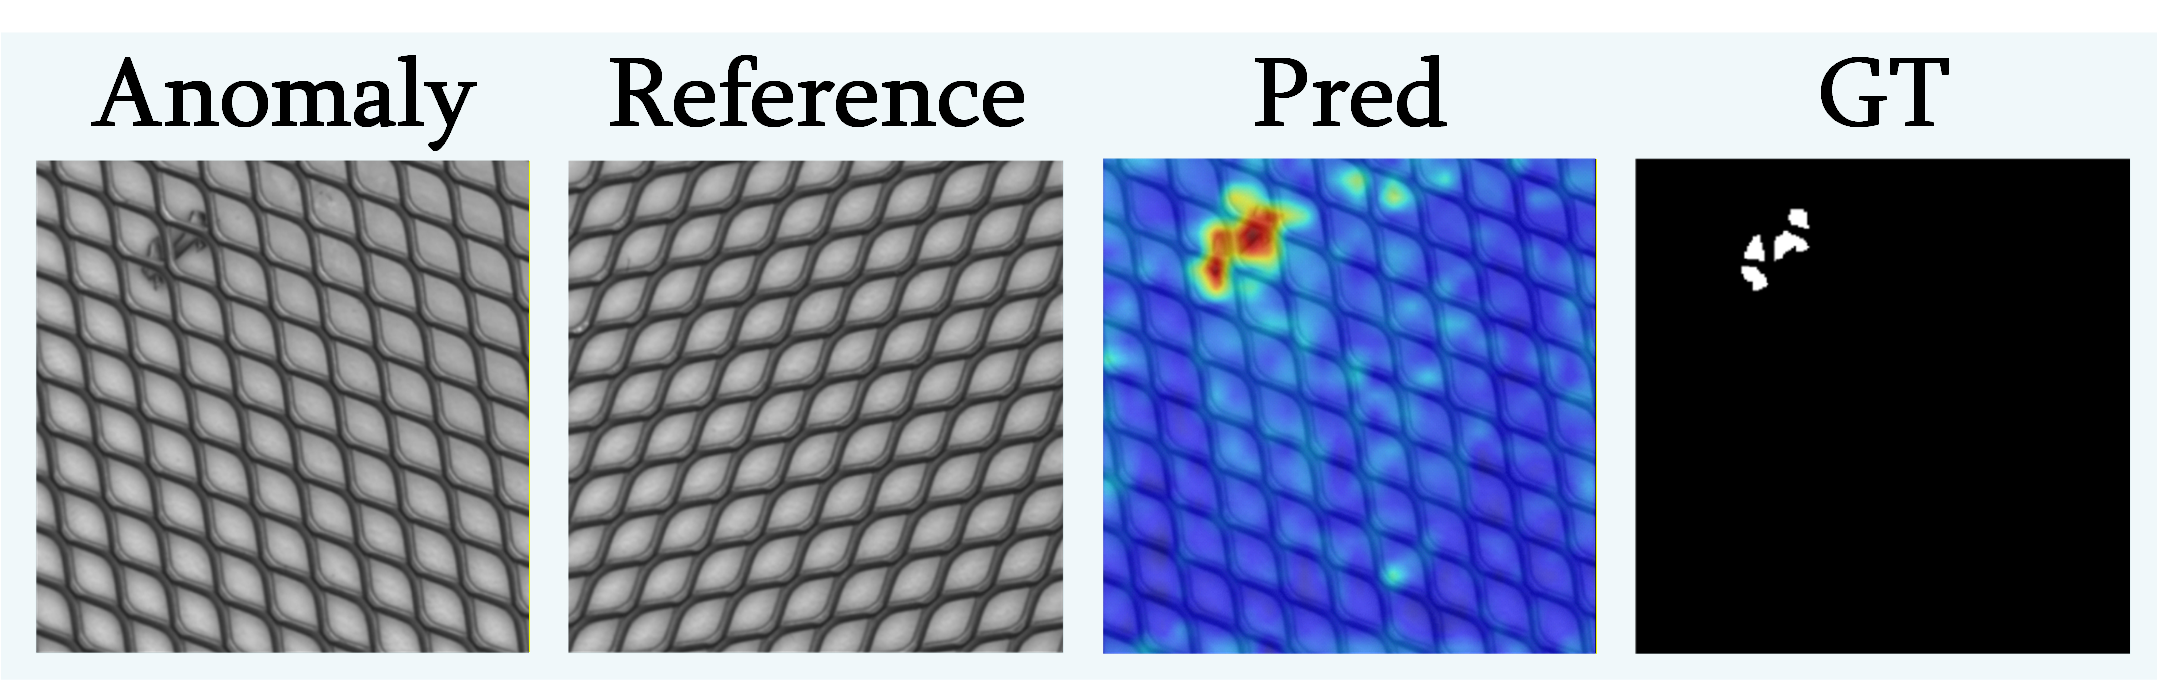
\includegraphics[width=1\linewidth]{figure/Figure_RAD.png}
    %\vspace{-6mm}
    \caption{Visualizations of MUAD with only one reference by RAD.}
    \label{fig:Figure_RAD}
    % \vspace{-10mm}
\end{figure}

In this work, we analyze the behavior of reconstruction-based MUAD in representation space, and show for the first time that these methods suffer from an inherent \textit{fidelity–stability dilemma}.
% In this work, we provide the first representation-space analysis of the inherent fidelity–stability dilemma in reconstruction-based MUAD.
% \looseness=-1
They must simultaneously achieve high-fidelity reconstruction of anomaly-free features (towards identity mapping) and stable residual scores under benign variations (a clear boundary between normal and abnormal). We show that these two training objectives are naturally contradictory and eventually lead to the \emph{dilemma} as discussed in Sec. \ref{sec:theory}. When high-fidelity reconstruction is enforced, the decoder must amplify small benign variations in encoder features, making the decision boundary highly sensitive. Conversely, relaxing reconstruction pressure improves stability but introduces a systematic approximation gap on the anomaly-free distribution, diluting residual-based anomaly evidence. 


% \looseness -1 
Motivated by this dilemma, we abandon decoder-based reconstruction and instead use a frozen off-the-shelf encoder together with a memory bank of anomaly-free encoder features.  Our key idea is to score anomalies purely by retrieval: given a test image, we compare its encoder features only to those stored in this memory, without learning a decoder or explicit density. We instantiate this idea in RAD (Retrieval-based Anomaly Detection), a \emph{training-free} MUAD framework. Concretely, RAD performs multi-level “global-then-patch” retrieval for anomaly scoring: for each test sample, it first retrieves a small set of globally compatible anomaly-free reference images, restricting comparisons to features that match its global context and spatial layout, and then scores each patch by matching it to patches from these references. RAD can adapt to new data simply by updating the memory bank rather than retraining, naturally accommodating new categories and distribution shifts; it also directly benefits from stronger frozen encoders as they become available, as confirmed by our experiments in Sec. \ref{sec:exp&analysis}.



We further provide a theoretical analysis showing that, when sharing the same frozen encoder and anomaly-free training set, retrieval-based anomaly scores provably upper-bound reconstruction-based residual scores, thereby avoiding the \emph{fidelity–stability dilemma} induced by information loss in decoder-based reconstruction. Empirically, RAD is, to our knowledge, the first training-free MUAD framework that consistently surpasses training-based methods, achieving state-of-the-art performance on four benchmarks~\cite{bergmann2019mvtec,zou2022spot,wang2024real,mchard20253d} under both standard multi-class and few-shot MUAD settings. We visualize how RAD accurately localizes anomalies on MVTec (see Fig.~\ref{fig:Figure_RAD}).
It remains accurate even with a single anomaly-free reference whose appearance differs from the test sample. These results provide a strong counterexample to the prevailing belief that MUAD requires heavy task-specific training, demonstrating that competitive, state-of-the-art anomaly detection is possible without training. %—raising the broader question: \emph{is domain-specific training truly necessary for strong anomaly detection?} 


% \looseness -1 
Specifically, our main contributions are: (i) Analyzing the fidelity–stability dilemma in encoder–decoder MUAD.
(ii) Proposing RAD, the first training-free MUAD framework that achieves state-of-the-art results.
(iii) We prove that, under a fair-comparison setting, retrieval-based scoring upper-bounds reconstruction residuals and thereby avoids the fidelity–stability trade-off.


%Looking ahead, we hope that our retrieval-based scoring approach will pave the way for new advancements in training-free MUAD research and motivate the community to re-examine of whether domain-specific training is necessary for strong anomaly detection.



% Our main contributions are:
% (i) We revisit encoder--decoder MUAD methods through the lens of a \emph{fidelity--stability dilemma}.
% (ii) We introduce RAD, the first training-free unified MUAD pipeline, superiors training-based methods and achieves state-of-the-art performance on four benchmarks across both standard and few-shot anomaly detection settings.
% (iii) We provide a theoretical analysis under a fair-comparison setting, showing that retrieval-based anomaly scoring upper-bounds reconstruction-based residual scoring and provably avoids the fidelity--stability trade-off.





% \vspace{-1.5mm}
\section{Fidelity-Stability Dilemma}
\label{sec:theory}


% \vspace{-1mm}
% \looseness=-1
In this section, we analyze encoder–decoder methods from the view of representation space and show they inherently face a fidelity–stability dilemma. We first show that, even on anomaly-free patches, the optimal reconstruction map generally deviates from the identity, so residuals remain non-zero due to unavoidable reconstruction errors. We then study how enforcing high-fidelity reconstruction of benign feature variations interacts with the bottleneck, and derive a lower bound that ties this requirement to the decoder’s local gain, revealing a fundamental fidelity–stability trade-off in residual scores.



% \paragraph{Problem Formulation.}
% Let $\mathcal{D}_{\mathrm{norm}}^{\mathrm{img}}=\{x_i\}_{i=1}^N$ be a dataset of $N$ anomaly-free training images, drawn i.i.d.\ from an anomaly-free distribution.
% Each image is decomposed into patches on a fixed grid, and we denote by
% $\mathcal{D}_{\mathrm{norm}}^{\mathrm{patch}}$ the resulting set of anomaly-free training patches.
% In contrast, test images may contain unseen defects, with some patches anomalous and others normal.
% Given a test image $x$, a detector produces an anomaly score $S(x,t)$ of each patch $t$.
% For the theoretical analysis below, we fix a test image and a patch and write $S(t)$ for the corresponding patch-wise anomaly scores.
% \vspace*{-2.4mm}
\paragraph{Problem formulation.}
Let $\mathcal{D}_{\mathrm{norm}}^{\mathrm{img}} = \{x_i\}_{i=1}^N$ be a dataset of $N$ anomaly-free training images covering a variety of classes. Each image is decomposed into patches on a fixed grid, and we denote by $\mathcal{D}_{\mathrm{norm}}^{\mathrm{patch}}$ the resulting set of anomaly-free training patches.
In contrast, test images may contain unseen defects, with some patches anomalous and others normal.
Given a test image $x$, a detector produces an anomaly score $S(x,t)$ for each patch $t$.
For the theoretical analysis below, we fix a test image and a patch and write $S(t)$ for the corresponding patch-wise anomaly score.



%The resulting score map is upsampled to pixel resolution and aggregated into an image-level score, for example by averaging the top $1\%$ pixel scores.
% \subsection{Reconstruction: Stability vs. Fidelity}
% \label{subsec:recon}
% \vspace{-2mm}
\paragraph{Reconstruction-based scoring.}
% Current state-of-the-art reconstruction methods~\cite{you2022unified,guo2025dinomaly,zhang2023exploring} use a training paradigm that freezes a pre-trained encoder $\Phi$ and learns a decoder $\Psi_\theta$ with an information-losing bottleneck $B$ applied in feature space.


Current state-of-the-art reconstruction methods~\cite{you2022unified,guo2025dinomaly,zhang2023exploring} use a training paradigm that freezes a pre-trained encoder $\Phi$ and learns a decoder $\Psi_\theta$ that approximately inverts an information-losing bottleneck $B$, aiming to reconstruct the encoder features from their bottlenecked versions.


To prevent the decoder from trivially copying $\Phi(n)$, the bottleneck $B$ stochastically removes or perturbs part of the representation, so that the decoder must infer missing information from the learned anomaly-free patterns rather than simply act as an exact identity mapping.
% At inference time, stochastic perturbations in $B$ are optionally disabled, and we still denote the resulting deterministic map by $B$.
The reconstruction path can then be written as $R_\theta(n) = \Psi_\theta\big(B(\Phi(n))\big)$.
The decoder is trained on anomaly-free patches by: 
\begin{equation}
\theta^* = \arg\min_\theta
    \sum_{n \in \mathcal{D}_{\mathrm{norm}}^{\mathrm{patch}}}
    \ell_{\mathrm{rec}}\big(\Phi(n),\, R_\theta(n)).
\end{equation}

Here $\theta^*$ represents the (ideal) best decoder parameters achievable under this objective, and $R_{\theta^*}$ is the corresponding optimal reconstruction decoder for anomaly-free patches. At test time, we use $R_{\theta^*}$ to reconstruct each patch $t$, defining the anomaly score as the feature residual
$
    S_{\mathrm{rec}}(t) = \big\|\Phi(t) - R_{\theta^*}(t)\big\|.
$
\label{eqa:residual_score}




To analyze equation \ref{eqa:residual_score}, we study the reconstruction map $R_{\theta^*}$
in feature space: (i) its nominal deviation from the identity on anomaly-free features, and (ii) how benign feature variations are propagated through the bottleneck–decoder pipeline. We begin by decomposing $R_{\theta^*}$
on anomaly-free patches into an identity term plus a reconstruction error.




\begin{figure*}
    \centering
    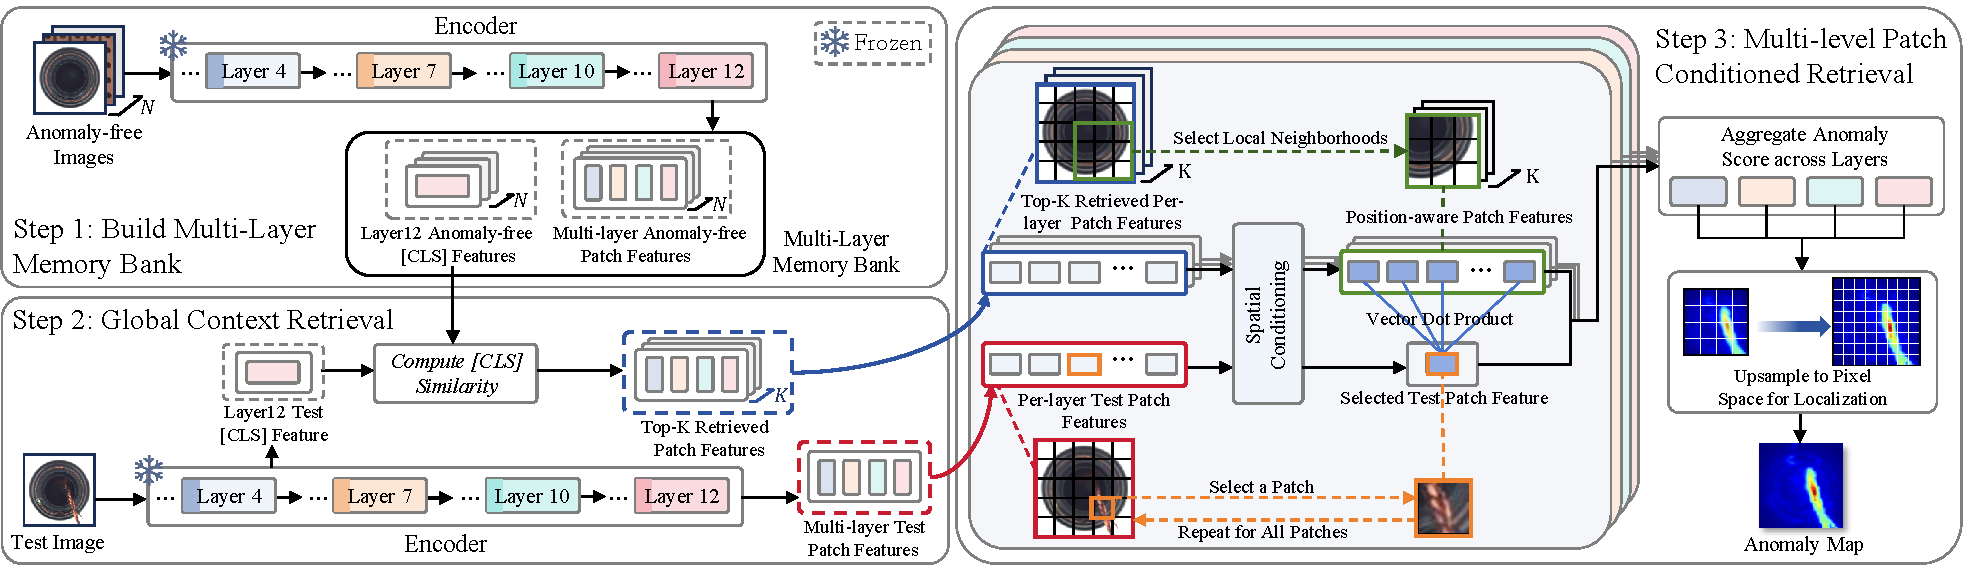
\includegraphics[width=1\linewidth]{figure/figure_framework.pdf}
    %\vspace{-6mm}
    \caption{Overview of the proposed RAD framework.}
    \label{fig:Figure_fw}
    % \vspace{-5mm}
\end{figure*}

% \vspace{-2mm}
\paragraph{Reconstruction as amortized inverse.}
% Viewing the test-time reconstruction purely as a function of encoder features, we have
% \begin{equation}
%     R_{\theta^*}(p) = \Psi_{\theta^*}\big(B(\Phi(p))\big).
% \end{equation}
For anomaly-free patches $n \in \mathcal{D}^{patch}_{\mathrm{norm}}$, the ideal behavior would be $R_{\theta^*}(n) = \Phi(n)$.
In practice, the information loss in $B$, finite capacity, and imperfect optimization jointly induce a systematic deviation from the identity, which we write as
\begin{equation}
    R_{\theta^*}(n) = \Phi(n) + \varepsilon_{\mathrm{approx}}(n),
    \qquad n \in \mathcal{D}_{\mathrm{norm}}^{\mathrm{patch}},
\end{equation}
% where $\varepsilon_{\mathrm{approx}}(n)$ aggregates approximation effects.

% We refer to $\varepsilon_{\mathrm{approx}}(n)$ as the per-patch \emph{approximation error}.
% Its magnitude,
% \(
% g(n)\triangleq \|\varepsilon_{\mathrm{approx}}(n)\|
% \),
% is the \emph{approximation gap} on patch $n$, and we denote the dataset-average gap by
% \(
% \Delta_{\mathrm{app}} \triangleq \mathbb{E}_{n\sim \mathcal{D}^{\mathrm{patch}}_{\mathrm{norm}}}\, g(n).
% \)


% Thus the reconstruction path acts as an amortized, biased memory of the anomaly-free feature manifold rather than an exact copy, and the size and structure of $\varepsilon_{\mathrm{approx}}$ determine how reconstruction fidelity trades off against the stability of the residual score $S_{\mathrm{rec}}(t)$.



% We refer to $\varepsilon_{\mathrm{approx}}(n)$ as the per-patch \emph{approximation error}.
% Its magnitude $g(n)\triangleq \|\varepsilon_{\mathrm{approx}}(n)\|$ is the \emph{approximation gap} on patch $n$,
% and we denote the dataset-average gap by
% $\Delta_{\mathrm{app}} \triangleq \mathbb{E}_{n\sim \mathcal{D}^{\mathrm{patch}}_{\mathrm{norm}}}\, g(n)$.
% Notably, for anomaly-free patches, the residual score satisfies
% $S_{\mathrm{rec}}(n)=\|\Phi(n)-R_{\theta^*}(n)\|=\|\varepsilon_{\mathrm{approx}}(n)\|$.
% \vspace{-2mm}
We refer to $\varepsilon_{\mathrm{approx}}(n)$ as the per-patch \emph{reconstruction error} in feature space.
Its magnitude $\alpha(n) \triangleq \|\varepsilon_{\mathrm{approx}}(n)\|$ is the \emph{reconstruction gap} on patch $n$.
Notably, for anomaly-free patches, the residual score satisfies
\[
S_{\mathrm{rec}}(n)
= \|\Phi(n)-R_{\theta^*}(n)\|
= \|\varepsilon_{\mathrm{approx}}(n)\|
= \alpha(n).
\]



% \vspace{-2mm}
% Thus the reconstruction path acts as an amortized, biased memory of the anomaly-free feature distribution rather than an exact copy.
Thus the reconstruction path acts as an amortized, biased inverse of the
bottlenecked encoder on the anomaly-free feature manifold rather than an exact
identity.
Moreover, both the \emph{magnitude} of $\varepsilon_{\mathrm{approx}}$ (captured by $\alpha(n)$) and its \emph{geometry} across $n$
(e.g., which feature directions are systematically distorted)
govern how reconstruction fidelity trades off against the stability of the residual score $S_{\mathrm{rec}}(t)$.






% \paragraph{Decoder amplification under information loss.}
% We now show that the decoder must act analogously to a high-gain amplifier.
% %
% For an anomaly-free patch $n \in \mathcal{D}_{\mathrm{norm}}^{\mathrm{patch}}$, 
% we let $\mathcal{V}_n \subset \mathbb{R}^D$ denote a subspace of benign feature 
% variations around $\Phi(n)$ that should not be treated as anomalies, 
% intuitively capturing feature differences between $\Phi(n)$ and feature vectors 
% $\Phi(n) + \delta$ of nearby anomaly-free patches. 
% % To formalize this, we define the feature reconstruction map $R = \Psi \circ B$ operated on encoder features and $F(n) = B(\Phi(n))$.
% % We focus on the local behavior of $R$ on benign variations around $\Phi(n)$, which is described by the Jacobian $J_R(\Phi(n))$.
% % By the chain rule, this Jacobian factorizes as
% % \begin{equation}
% %     J_R(\Phi(n)) = J_\Psi\big(F(n)\big)\, J_B\big(\Phi(n)\big).
% % \end{equation}
% Let $R = \Psi \circ B$ denote the feature reconstruction map.
% For an anomaly-free patch $n\in \mathcal{D}_{\mathrm{norm}}^{\mathrm{patch}}$, let $\mathcal{V}_n\subset \mathbb{R}^D$ be a subspace of benign feature variations around $\Phi(n)$.
% By the chain
% rule, the Jacobian of $R$ at $\Phi(n)$ factorizes as
% \begin{equation}
% \label{eq:chainrule}
%     J_R(\Phi(n)) = J_\Psi\!\big(B(\Phi(n))\big)\, J_B\!\big(\Phi(n)\big).
% \end{equation}



\paragraph{Decoder amplification under information loss.}
Let $R = \Psi \circ B$ denote the feature reconstruction map and $\mathcal{V}_n \subset \mathbb{R}^D$ be a subspace of benign feature
variations around $\Phi(n)$ that should not be treated as anomalies, e.g.,
feature differences between $\Phi(n)$ and $\Phi(n)+\delta$ for nearby
anomaly-free patches.
We write $J_R(u)$ for the Jacobian of the map $R$ evaluated at $u$ (and similarly
$J_\Psi(u)$ and $J_B(u)$).
By the chain rule,
\begin{equation}
    J_R(\Phi(n)) = J_\Psi\big(B(\Phi(n))\big)\, J_B\big(\Phi(n)\big).
\label{eq:chainrule}
\end{equation}

% We denote by $D R(n)$ the Jacobian of the map $R$ at $n$, and similarly
% $D\Psi(n)$ and $D B(n)$.
% By the chain rule,
% \begin{equation}
% \label{eq:chainrule}
%     D R(\Phi(n))
%     = D\Psi\big(B(\Phi(n))\big)\, D B\big(\Phi(n)\big).
% \end{equation}
% \vspace{-2mm}
This decomposition allows us to convert the fidelity requirement on $R$
(Assumption~\ref{ass:fidelity}) and the contraction induced by $B$
into a lower bound on the decoder gain $J_\Psi$.





\begin{assumption}[anomaly-free feature fidelity]
\label{ass:fidelity}
Fix a fidelity parameter $\eta \in (0,1)$, which upper-bounds the relative reconstruction error on benign feature variations, with the high-fidelity regime corresponding to $\eta \ll 1$.
For each anomaly-free training patch $n \in \mathcal{D}_{\mathrm{norm}}^{\mathrm{patch}}$, there exists a radius $r>0$ such that for all benign feature perturbations $\delta \in \mathcal{V}_n$ with $\|\delta\|\le r$,
\begin{equation}
    \big\| R(\Phi(n)+\delta) - R(\Phi(n)) - \delta \big\| \le \eta \|\delta\|.
\end{equation}
% \vspace{-2mm}
Equivalently, the Jacobian of $R_{\theta^*}$ restricted to $\mathcal{V}_n$ satisfies
\begin{equation}
    \sigma_{\min}\big(J_{R}(\Phi(n))\big|_{\mathcal{V}_n}\big) \ge 1 - \eta,
\end{equation}
% \vspace{-2mm}
where $\sigma_{\min}(\cdot)$ is the smallest singular value.
\end{assumption}


Assumption~\ref{ass:fidelity} enforces a local near-identity regime: the reconstruction map preserves benign feature variations in $\mathcal{V}_n$ up to relative error $\eta$, which is the formal notion of high-fidelity reconstruction used in our amplification analysis.


\begin{lemma}[Decoder amplification]
\label{lem:amplification}
Under Assumption~\ref{ass:fidelity}, the decoder Jacobian satisfies
\begin{equation}
    \sigma_{\max}\big(J_\Psi(B(\Phi(n)))\big)
    \;\ge\;
    \frac{1-\eta}{
    \sigma_{\min}\big(J_B(\Phi(n))\big|_{\mathcal{V}_n}\big)},
\end{equation}
% \vspace{-1mm}
where $\sigma_{\max}(\cdot)$ is the largest singular value.
\end{lemma}

\emph{Proof sketch.}
Restrict all operators to the subspace $\mathcal{V}_n$.
For matrices $A,B$, one has $\sigma_{\min}(AB) \le \sigma_{\max}(A)\,\sigma_{\min}(B)$.
% Applying this to $A = J_\Psi(F(n))$ and $B = J_B(\Phi(n))|_{\mathcal{V}_n}$ and using $J_R = J_\Psi J_B$ yields
% \[
% \sigma_{\min}\big(J_R|_{\mathcal{V}_n}\big)
% \le \sigma_{\max}\big(J_\Psi(F(n))\big)\,
%    \sigma_{\min}\big(J_B(\Phi(n))\big|_{\mathcal{V}_n}\big).
% \]
Applying this to $A = J_\Psi\big(B(\Phi(n))\big)$ and 
$B = J_B\big(\Phi(n)\big)\big|_{\mathcal{V}_n}$ and using
% \[
% J_R\big(\Phi(n)\big) = J_\Psi\big(B(\Phi(n))\big)\,J_B\big(\Phi(n)\big)
% \]
Eq.~\ref{eq:chainrule}
yields
% \[
% \sigma_{\min}\big(J_R\big(\Phi(n)\big)\big|_{\mathcal{V}_n}\big)
% \le \sigma_{\max}\big(J_\Psi(B(\Phi(n)))\big)\,
%    \sigma_{\min}\big(J_B(\Phi(n))\big|_{\mathcal{V}_n}\big).
% \]
\begin{equation}
\resizebox{0.9\linewidth}{!}{$
\sigma_{\min}\big(J_R(\Phi(n))\big|_{\mathcal{V}_n}\big)
\le
\sigma_{\max}\big(J_\Psi(B(\Phi(n)))\big)\,
\sigma_{\min}\big(J_B(\Phi(n))\big|_{\mathcal{V}_n}\big)
$}
\end{equation}


Rearranging and invoking Assumption~\ref{ass:fidelity} finishes the proof (see Appendix Sec.~\ref{sec:proof} for the full proof). Thus, for a strong bottleneck, the restricted smallest singular value
$\sigma_{\min}(J_B(\Phi(n))|_{\mathcal{V}_n})$ can be very small since $B$ removes or compresses information along many benign feature variations.
Lemma~\ref{lem:amplification} then implies that the decoder must have a large $\sigma_{\max}(J_\Psi)$ in order to maintain high-fidelity reconstruction on anomaly-free patches, which makes it behave as a high-gain amplifier.



% In feature space, reconstruction is a biased, amortized memory of normality, so residuals on anomaly-free patches are driven by approximation error; enforcing variation preservation through an information-losing bottleneck turns the decoder into a high-gain amplifier, making residuals unstable to benign perturbations. This is the stability–fidelity dilemma. In the next section we contrast this with retrieval, which replaces learning-based approximation with a memory of anomaly-free distribution and therefore sidesteps the dilemma.


% In feature space, reconstruction is a biased, amortized memory of normality, so residuals on anomaly-free patches are driven by approximation error; enforcing variation preservation through an information-losing bottleneck turns the decoder into a high-gain amplifier, making residuals unstable to benign perturbations. 
% \looseness -1 
In feature space, reconstruction acts as a biased, amortized inverse of the bottlenecked encoder on normal features, so residuals on anomaly-free patches are driven by reconstruction error; enforcing variation preservation through an information-losing bottleneck forces the decoder into a high-gain amplifier, making residuals unstable to benign perturbations.
Consequently, either many anomaly-free patches acquire large residuals and are incorrectly flagged as anomalous, or strong regularization makes the decoder overly smooth so that small defects are reconstructed together with benign variations and go undetected. This stability--fidelity dilemma echoes the stability--accuracy trade-off for deep inverse problems~\cite{colbrook2022difficulty}, but here it appears directly in patch-wise reconstruction scores for anomaly detection. In the next section we show that retrieval-based scoring, which replaces learning-based approximation with an explicit memory of anomaly-free features, sidesteps this dilemma.



% \vspace{-2mm}
\section{RAD: Towards Training-free MUAD}
\label{sec:evoad}
% \vspace{-1mm}
In this section, we formalize the retrieval-based view of RAD and derive its concrete multi-level design. We begin by constructing an explicit multi-layer memory of anomaly-free features that serves as the reference bank for all subsequent retrieval operations (Sec.~\ref{sec:memory}). Building on this, a global context retrieval stage selects a small, semantically compatible reference set for each test image (Sec.~\ref{sec:cls-retrieval-subsec}). We then describe multi-level conditional patch retrieval and anomaly scoring, where spatially conditioned patch matching is performed within local neighborhoods and scores are fused across layers into dense anomaly maps (Sec.~\ref{sec:retrieval}).



% \subsection{The Oracle Anomaly Score}
% \label{sec:prelim}

% We first formalize an ideal, layer-wise patch anomaly score in feature space. 
% At a given encoder layer $\ell$, let $z \in \mathbb{R}^{d_\ell}$ denote a patch
% embedding, $g$ a global descriptor that summarizes the image-level context, and
% $s$ the patch location on the token grid.
% Under the normality hypothesis (i.e., assuming the image is anomaly-free), we posit a conditional distribution
% \begin{equation}
% p_{0,\ell}(z \mid g,s),
% \end{equation}
% at layer $\ell$, where the subscript $0$ indicates the (normal) null model.
% We interpret $p_{0,\ell}(z \mid g,s)$ as the normal-data density of patch embeddings given $(g,s)$.
% We then define the ideal anomaly score as the conditional negative
% log-likelihood
% \begin{equation}
% S^{\star}_\ell(z,g,s) := -\log p_{0,\ell}(z \mid g,s),
% \end{equation}
% which coincides with the self-information of $z$ under the normal-data
% distribution, so patches that are unlikely under $p_{0,\ell}(\cdot \mid g,s)$
% receive higher scores and are treated as more anomalous.

% In RAD, we do not estimate $p_{0,\ell}$ explicitly; instead, we design a
% retrieval-based surrogate score that increases when a patch is poorly supported
% by nearby normal features in memory, serving as a training-free approximation
% to $S^{\star}_\ell(z,g,s)$.

% \vspace{-1mm}
\subsection{Multi-layer Anomaly-free Feature Memory Bank}
\label{sec:memory}
Features from different encoder layers provide complementary similarity signals~\cite{park2023self,amir2022effectiveness}. Shallow and intermediate layers retain high-frequency, local information such as edges and small geometric deviations, such that similarity is sensitive to subtle surface changes. Deeper layers aggregate information over larger receptive fields and become more invariant to low-level appearance, so similarity instead reflects semantic and structural consistency rather than precise texture.

For multi-class anomaly detection (MUAD), this complementarity is crucial. Fine-grained defects such as scratches, or small dents are best captured by shallow and intermediate features, while larger structural changes or misalignments are more naturally expressed in deeper semantic features. By retrieving and scoring patches jointly across multiple layers, RAD combines the sensitivity of shallow features with the robustness and semantic context of deeper ones, leading to more reliable localization of both subtle surface anomalies and larger structural defects.


Concretely, we instantiate this idea by constructing a multi-layer memory bank of anomaly-free features.
Let $\Phi$ be a frozen encoder, and let $\mathcal{L}$ be a small set of encoder layers chosen for multi-layer feature extraction. For each anomaly-free image $x_i$, we pass $x_i$ through $\Phi$ and take the \texttt{[CLS]} token of the final hidden state, apply $\ell_2$ normalization, and  store it as a global descriptor $g(x_i)$, representing the entire input as a compact, global summary. These descriptors are later used for global context retrieval in Sec.~\ref{sec:cls-retrieval-subsec}.
In addition, we store all $\ell_2$-normalized patch embeddings $z^{(\ell)}(x_i) \in \mathbb{R}^{d_\ell}$ at layers $\ell \in \mathcal{L}$, which are later used for conditioned retrieval and scoring in Sec.~\ref{sec:retrieval}.
These stored features form a multi-layer memory bank of anomaly-free representations that enables the training-free advantage of RAD.

% \vspace{-2mm}
\subsection{Global Context Conditioned Retrieval}
\label{sec:cls-retrieval-subsec}
% A naive patch-retrieval scheme would compare each test patch against all normal patches in the memory bank, regardless of which semantic class they belong to.
% In a multi-class AD setting, this leads to two problems: (i) patches from semantically unrelated classes (e.g., different products) can become nearest neighbors, corrupting the approximation to the conditional normal density $p_{0,\ell}(\cdot \mid g,s)$, and (ii) the candidate set grows linearly with the total memory size, increasing computation.
% To approximate conditioning on the global context $g$ introduced in Sec.~\ref{sec:prelim}, RAD therefore first performs a coarse, global retrieval step that filters the memory to a small set of semantically compatible reference images.
A naive patch-retrieval scheme would compare each test patch against all normal patches in the memory bank, regardless of their semantic class. In the MUAD setting, this leads to two problems: (i) patches from semantically unrelated classes can become nearest neighbors, introducing severe semantic mismatch, and (ii) the candidate set grows linearly with the total memory size, increasing computation. To address this, RAD first performs a coarse global retrieval step that filters the memory to a small set of semantically compatible reference images.


As shown in Figure~\ref{fig:Figure_fw}, for each anomaly-free global descriptor $g(x_i)$ in the memory bank, given a test image $x$, we compute the cosine similarity between them as $\label{eq:cls-retrieval}
\mathrm{sim}_i(x)
:=
\big\langle g(x),\, g(x_i) \big\rangle.$
We then define $\mathcal{N}_K(x)
:=
\operatorname{TopK}\big(\{\mathrm{sim}_i(x)\}_{i=1}^{N}\big),$
as the indices of the $K$ most similar anomaly-free images to $x$.
All subsequent patch comparisons at any layer $\ell \in \mathcal{L}$ are restricted to images in $\mathcal{N}_K(x)$, enforcing semantic consistency and reducing computation.


We use only the last-layer \texttt{[CLS]} token as $g(x_i)$ because it provides a semantically rich global summary of the image, optimized during pretraining to capture high-level category and scene information. In MUAD, this semantic descriptor lets us retrieve a few globally similar reference images from a heterogeneous memory bank, suppressing features from unrelated classes before patch-level matching. Low- and mid-level cues are already handled by the multi-layer patch memory, so adding additional global tokens from earlier layers would increase complexity without clear benefit.

% \vspace{-2mm}
\subsection{Patch-level Conditioned Retrieval and Scoring}
\label{sec:retrieval}

On the global context retrieved subset $\mathcal{N}_K(x)$, RAD performs
patch-level conditioned retrieval and scoring independently based on multi-layer features.
For clarity, we first describe the procedure for a layer
$\ell \in \mathcal{L}$; the same steps are then applied in parallel to all
layers in $\mathcal{L}$, and the resulting scores are fused across layers.

% \looseness -1 
\paragraph{Spatial conditioning via local neighborhoods.}

% Even within the retrieved subset $\mathcal{N}_K(x)$, unconstrained patch
% matching across all spatial locations may pair semantically unrelated parts,
% which breaks the intended conditioning on the patch position $s$.
% To alleviate this, RAD enforces coarse spatial consistency via a local
% neighborhood on the token grid.

% \vspace{-3mm}
% \looseness -1 
In anomaly detection, objects are typically roughly aligned, and different regions of the image correspond to different functional parts (e.g., screw vs.\ background).
Matching a query patch against anomaly-free patches from arbitrary locations, even within the global context conditioned retrieved set $\mathcal{N}_K(x)$, therefore risks pairing semantically unrelated parts, which can distort anomaly scores. Thus, we argue that patch matching should be conditioned by \emph{where} a patch appears in the image.

% \looseness -1 
To implement this inductive bias, RAD imposes a spatial prior. A patch should be compared only to anomaly-free patches from a local neighborhood around the same grid location.
This preserves coarse spatial semantics while remaining robust to small misalignments and viewpoint changes.


% \looseness -1 
Formally, we view a test image $x$ as an $H \times W$ grid of patches and let
$t \leftrightarrow (h_t, w_t)$ index patch $t$.
For each layer $\ell$, the memory bank stores anomaly-free patch embeddings
$\{z^{(\ell)}_n\}$, where each $z^{(\ell)}_n$ comes from a patch at spatial
coordinates $(h_n, w_n)$ in a anomaly-free image.
Given a neighborhood radius $\rho \in \mathbb{Z}_{\ge 0}$, define $\mathcal{P}_\rho(t)
:=
\Big\{ n : \big\|(h_n, w_n) - (h_t, w_t)\big\|_\infty \le \rho \Big\}$ as the set of anomaly-free within an $\ell_\infty$-ball of radius $\rho$
around $t$.
For layer $\ell$ and retrieved image indices $\mathcal{N}_K(x)$, we then form
the position-aware candidate set of $\ell_2$-normalized anomaly-free patch embeddings
\begin{equation}
\label{eq:cand-set}
\mathcal{M}_\ell(x,t)
:=
\Big\{ z^{(\ell)}_{n} : n \in \mathcal{P}_\rho(t),\ i(n) \in \mathcal{N}_K(x) \Big\},
\end{equation}
% \looseness=-1
where $i(n)$ is the index of the image from which patch $n$ is extracted.
Thus $\mathcal{M}_\ell(x,t)$ restricts patch matching to patches that are semantically and spatially aligned.


% \vspace{-2mm}
\paragraph{Multi-layer Anomaly Scoring.}
Given the globally and spatially conditioned candidate set $\mathcal{M}_\ell(x,t)$, RAD assigns each test patch an anomaly score by measuring how well it is supported by retrieved features.
For a layer $\ell$ test patch embedding $z^{(\ell)}_{t}(x)$ at location $t$ in image $x$, we define the layer-wise anomaly score via 1-NN cosine dissimilarity:
\begin{equation}
\label{eq:patch-energy-cos}
S_\ell(x,t)
:= 1 - \max_{z \in \mathcal{M}_\ell(x,t)}
\left\langle z^{(\ell)}_{t}(x), z \right\rangle.
\end{equation}
If a test patch is well supported by retrieved features, it admits a close neighbor in $\mathcal{M}_\ell(x,t)$ and thus a small $S_\ell(x,t)$, whereas patches that deviate from the local anomaly-free distribution yield larger $S_\ell(x,t)$.

To aggregate evidence across layers, we adopt a simple weighted fusion and combine the layer-wise scores as
\begin{equation}
S(x,t)
:=
\sum_{\ell \in \mathcal{L}} w_\ell \, S_\ell(x,t),
\quad
w_\ell \ge 0,\ \sum_{\ell \in \mathcal{L}} w_\ell = 1.
\end{equation}

Each layer thus contributes as an expert in its own feature space, and the fused patch scores $S(x,t)$ are finally upsampled to pixel space for localization, while image-level anomaly scores are obtained by pooling.




% \subsection{Computational Efficiency}
% \label{sec:efficiency}

% We finally compare the computational cost of EvoAD to naive global patch
% search.
% A naive approach compares each query patch against all normal patches, i.e.,
% $N \times P$ candidates per query, leading to
% $O(NP^2 C_\ell)$ similarity evaluations per layer for dense localization,
% where $C_\ell$ denotes the per-pair matching cost at layer $\ell$.

% In contrast, EvoAD decomposes matching into two stages, summarized in
% Alg.~\ref{alg:condpatchknn}.
% First, CLS retrieval performs a coarse screening over $N$ normal images with
% cost $O(N C_{\ell^\star})$ per test image.
% Second, patch matching is carried out only within the retrieved $K$ images and
% within a local neighborhood on the patch grid.
% For each patch $q$, the candidate count becomes
% \begin{equation}
% |\mathcal{M}_\ell(x,q)|
% =
% K \cdot |\mathcal{P}_\rho(q)|
% \approx K (2\rho + 1)^2,
% \end{equation}
% which is independent of $N$ and typically much smaller than $NP$.
% Accordingly, the per-layer matching cost is reduced from
% \[
% \underbrace{O(NP^2 C_\ell)}_{\text{naive global patch search}}
% \quad\rightarrow\quad
% \underbrace{O\!\big(P \cdot K (2\rho+1)^2 C_\ell\big)}_{\text{ours: retrieval + local neighborhood}},
% \]
% while CLS screening adds a one-time cost $O(N C_{\ell^\star})$ per test image.
% Overall, the per-image inference cost is
% \begin{equation}
% O\big(N C_{\ell^\star}\big)
% \;+\;
% \sum_{\ell\in\mathcal{L}} O\Big(P \cdot K (2\rho+1)^2 \cdot C_\ell\Big).
% \end{equation}
% Thus conditional retrieval avoids global patch search over the full normal
% pool, reduces the candidate scale per patch from $NP$ to $K(2\rho+1)^2$, and
% simultaneously improves robustness by enforcing context (via CLS retrieval)
% and coarse spatial consistency (via local neighborhoods).

% \begin{algorithm}[tb]
%   \caption{EvoAD}
%   \label{alg:condpatchknn}
%   \begin{algorithmic}
%     \STATE {\bfseries Input:} normal dataset $\mathcal{D}_0=\{x_i\}_{i=1}^{N}$, frozen encoder, layers $\mathcal{L}$, top-$K$, radius $\rho$, weights $\{w_\ell\}_{\ell\in\mathcal{L}}$
%     \STATE {\bfseries Offline:} store CLS tokens $\mathcal{B}_{\mathrm{cls}}^{(\ell)}$ and patch tokens $\mathcal{B}_{\mathrm{patch}}^{(\ell)}$ for all $\ell\in\mathcal{L}$
%     \STATE {\bfseries Test image} $x$: extract $\{g^{(\ell)}(x), Z^{(\ell)}(x)\}_{\ell\in\mathcal{L}}$ and $\ell_2$-normalize all tokens
%     \STATE {\bfseries CLS retrieval:} compute $\mathcal{N}_K(x)$ via Eq.~\eqref{eq:cls-retrieval}
%     \FOR{$q=1$ {\bfseries to} $P$}
%       \FORALL{$\ell\in\mathcal{L}$}
%         \STATE Form $\mathcal{M}_{\ell}(x,q)$ via Eq.~\eqref{eq:cand-set}
%         \STATE Compute $S_{\ell}(x,q)$ via Eq.~\eqref{eq:patch-energy-cos}
%       \ENDFOR
%       \STATE Fuse $S(x,q)\leftarrow \sum_{\ell\in\mathcal{L}} w_\ell\,S_{\ell}(x,q)$
%     \ENDFOR
%     \STATE {\bfseries Output:} patch score map $\{S(x,q)\}_{q=1}^{P}$
%   \end{algorithmic}
% \end{algorithm}

% \vspace{-2mm}
\section{Why is Retrieval Better?}
\label{sec:why-retrieval}
% \vspace{-1mm}
We now explain why, for the same encoder and training data, RAD avoids the fidelity--stability dilemma analyzed in Sec.~\ref{sec:theory}, and upper bounds encoder--decoder pipelines.


% \paragraph{Fidelity: Vanishing approximation error on anomaly-free embeddings.}
% % Both reconstruction-based and retrieval-based pipelines operate on the same set of anomaly-free training images. 
% Encoder–decoder methods attempt to internalize the anomaly-free patch distribution via a parametric, bottlenecked mapping, which inevitably incurs function-approximation error on the training embeddings due to information loss in the bottleneck (Sec.~\ref{sec:theory}). In contrast, RAD is training-free, and simply stores all anomaly-free embeddings in a memory bank and compares a test embedding to this empirical support. 


% Let $\mathcal{M}$ denote the set of stored anomaly-free embeddings, and define
% the retrieval score as the distance to the nearest neighbor in memory,
% $S_{\mathrm{ret}}(z) := \min_{u \in \mathcal{M}} \|z - u\|$, or an equivalent
% non-negative dissimilarity.
% If the memory contains every anomaly-free embedding $z_i \in \mathcal{M}$, then
% for each stored normal point we have $S_{\mathrm{ret}}(z_i) = 0$, since its
% nearest neighbor is itself.
% Thus retrieval incurs essentially zero empirical approximation error on the
% anomaly-free embeddings.
% No method that maps embeddings to non-negative anomaly scores can achieve
% strictly smaller empirical error on this set; at best it can match retrieval.
% This highlights a structural difference: approximation error on the
% anomaly-free manifold is controlled by the encoder--decoder’s capacity and
% bottleneck design, whereas RAD represents the anomaly-free distribution
% non-parametrically via its empirical support, without additional learning.
% \vspace{-2mm}
\paragraph{Fidelity: Empirical saturation on anomaly-free embeddings.}
% \looseness=-1
Encoder–decoder methods attempt to reconstruct anomaly-free patch embeddings
through a parametric, bottlenecked mapping, which inevitably incurs
function-approximation error on the training embeddings due to information loss
(Sec.~\ref{sec:theory}).
In contrast, RAD is training-free as it stores all anomaly-free embeddings in a
memory bank and defines the retrieval score as the distance to this empirical support.

Let $\gamma$ denote the set of stored anomaly-free embeddings, and define
$S_{\mathrm{ret}}(z) := \min_{u \in \gamma} \|z - u\|$, or an equivalent
non-negative dissimilarity.
% If the memory contains every anomaly-free embedding $z_i \in \gamma$, then for each stored normal point we have
Then for every stored normal embedding $z_i \in \gamma$ we have
$S_{\mathrm{ret}}(z_i) = 0$, since its
nearest neighbor is itself.
Thus retrieval incurs zero empirical reconstruction error on the anomaly-free embeddings.

More importantly, $S_{\mathrm{ret}}$ is the canonical distance-to-set function since it is non-negative, vanishes exactly on $\gamma$, and is $1$-Lipschitz in
feature space (Lemma~\ref{lem:nonexpansive}).
Any other anomaly score with these basic regularity properties must be
pointwise no larger than $S_{\mathrm{ret}}$.
% Thus, for a fixed encoder and dataset, retrieval saturates the
% best achievable fidelity on the empirical anomaly-free support among stable
% (non-expansive) feature-space scores, 
Thus, for a fixed encoder and dataset, retrieval saturates the best achievable empirical fidelity on the stored anomaly-free embeddings among stable (non-expansive) feature-space scores,
whereas encoder–decoder methods incur
additional approximation error from the learned bottlenecked decoder.


\begin{table*}[t]
\centering
\caption{Standard MUAD results.
Best results are highlighted in boldface, and the runner-up is underlined.}
% \vspace{-2mm}
\label{tab:muad_results}

\begingroup
\small                        
\setlength{\tabcolsep}{3.8pt}   
\renewcommand{\arraystretch}{1.15}
\setlength{\extrarowheight}{0.3ex}

\begin{tabular}{l c|cc|cc|cc}
\specialrule{1.2pt}{0pt}{2pt}

\multicolumn{2}{c|}{\textbf{Dataset} $\rightarrow$} &
\multicolumn{2}{c|}{MVTec-AD} &
\multicolumn{2}{c|}{VisA} &
\multicolumn{2}{c}{Real-IAD} \\
\specialrule{0.6pt}{2pt}{2pt}

\multicolumn{2}{c|}{\textbf{Metric} $\rightarrow$} &
\multicolumn{3}{c}{Image-level (I-AUROC/I-AP/I-$F_1$-max)} &
\multicolumn{3}{c}{Pixel-level (P-AUROC/P-AP/P-$F_1$-max/AUPRO)} \\
\specialrule{0.6pt}{2pt}{2pt}

\multicolumn{2}{c|}{\textbf{Method} $\downarrow$}  &
\multicolumn{1}{c}{Image-level} & \multicolumn{1}{c|}{Pixel-level} &
\multicolumn{1}{c}{Image-level} & \multicolumn{1}{c|}{Pixel-level} &
\multicolumn{1}{c}{Image-level} & \multicolumn{1}{c}{Pixel-level} \\
\specialrule{0.6pt}{2pt}{2pt}

\multicolumn{2}{c|}{RD4AD  \tiny \textit{CVPR'22}} &
94.6/96.5/95.2 & 96.1/48.6/53.8/91.1 &
92.4/92.4/89.6 & 98.1/38.0/42.6/91.8 &
82.4/79.0/73.9 & 97.3/25.0/32.7/89.6 \\

\multicolumn{2}{c|}{UniAD \tiny \textit{NIPS'22}}&
96.5/98.8/96.2 & 96.8/43.4/49.5/90.7 &
88.8/90.8/85.8 & 98.3/33.7/39.0/85.5 &
83.0/80.9/74.3 & 97.3/21.1/29.2/86.7 \\

\multicolumn{2}{c|}{SimpleNet \tiny \textit{CVPR'23}}&
95.3/98.4/95.8 & 96.9/45.9/49.7/86.5 &
87.2/87.0/81.8 & 96.8/34.7/37.8/81.4 &
57.2/53.4/61.5 & 75.7/2.8/6.5/39.0 \\

\multicolumn{2}{c|}{DeSTSeg \tiny \textit{CVPR'23}}&
89.2/95.5/91.6 & 93.1/54.3/50.9/64.8 &
88.9/89.0/85.2 & 96.1/39.6/43.4/67.4 &
82.3/79.2/73.2 & 94.6/37.9/41.7/40.6 \\

\multicolumn{2}{c|}{DiAD \tiny \textit{AAAI'24}}&
97.2/99.0/96.5 & 96.8/52.6/55.5/90.7 &
86.8/88.3/85.1 & 96.0/26.1/33.0/75.2 &
75.6/66.4/69.9 & 88.0/2.9/7.1/58.1 \\

\multicolumn{2}{c|}{MambaAD \tiny \textit{NIPS'24}}&
98.6/99.6/97.8 & 97.7/56.3/59.2/93.1 &
94.3/94.5/89.4 & 98.5/39.4/44.0/91.0 &
86.3/84.6/77.0 & 98.5/33.0/38.7/90.5 \\

\multicolumn{2}{c|}{OmiAD \tiny \textit{ICML'25}}&
98.8/99.7/98.5 & 97.7/52.6/56.7/93.2 &
95.3/96.0/91.2 & 98.9/40.4/44.1/89.2 &
\underline{90.1}/\underline{88.6}/\underline{82.8} & \underline{98.9}/37.7/42.6/93.1 \\

\multicolumn{2}{c|}{Dinomaly \tiny \textit{CVPR'25}}&
\textbf{99.6}/\textbf{99.8}/\textbf{99.0} &
\underline{98.4}/\underline{69.3}/\underline{69.2}/\underline{94.8} &
\textbf{98.7}/\textbf{98.9}/\textbf{96.2} &
\underline{98.7}/\underline{53.2}/\underline{55.7}/\underline{94.5} &
89.3/86.8/80.2 &
98.8/\underline{42.8}/\underline{47.1}/\underline{93.9} \\

\specialrule{0.6pt}{2pt}{3pt}

\rowcolor{blue!10}
\multicolumn{2}{c|}{\textbf{RAD (Ours)}} &
\textbf{99.6}/\textbf{99.8}/\textbf{99.0} &
\textbf{98.5}/\textbf{75.6}/\textbf{71.3}/\textbf{94.9} &
\underline{97.5}/\underline{97.3}/\underline{95.2} &
\textbf{99.1}/\textbf{55.3}/\textbf{57.5}/\textbf{94.6} &
\textbf{92.0}/\textbf{89.9}/\textbf{83.0} &
\textbf{99.1}/\textbf{53.7}/\textbf{54.2}/\textbf{96.1} \\

\specialrule{1.2pt}{2pt}{2pt}
% \vspace{-10mm}
\end{tabular}
\endgroup
\end{table*}

% \vspace{-2.5mm}
\paragraph{Inherited Stability.}
Retrieval also inherits a strong stability guarantee in feature space.
Because the encoder is frozen, the memory set $\gamma$ is fixed, and the
retrieval score is computed solely as a distance to this fixed set.
Hence, we obtain the following property.
% \vspace{-1mm}
\begin{lemma}[Non-expansiveness]
\label{lem:nonexpansive}
For any features $u,v, z \in \mathbb{R}^D$,
\begin{equation}
    \big|S_{\mathrm{ret}}(u) - S_{\mathrm{ret}}(v)\big|
    \le \|u - v\|.
\end{equation}
\end{lemma}
% \vspace{-2mm}
\emph{Proof.}
Let $a_v \in \arg\min_{z\in\gamma} \|v-z\|$.
By the triangle inequality,
$S_{\mathrm{ret}}(u) \le \|u-a_v\|
\le \|u-v\| + \|v-a_v\|
= \|u-v\| + S_{\mathrm{ret}}(v)$,
which yields $S_{\mathrm{ret}}(u) - S_{\mathrm{ret}}(v) \le \|u-v\|$.
Exchanging $u$ and $v$ gives the claim.

Lemma~\ref{lem:nonexpansive} shows that retrieval does not amplify benign perturbations in the encoder features as small changes in $z$ translate to at most equally small changes in $S_{\mathrm{ret}}(z)$; i.e. the variation in anomaly score between any two features is upper bounded by their feature-space distance.
This stands in sharp contrast to reconstruction-based anomaly scoring in
Sec.~\ref{sec:theory}, where information loss in the bottleneck forces the
decoder to have large Jacobian norm (Lemma~\ref{lem:amplification}), so the
residual score $S_{\mathrm{rec}}$ inevitably exhibits decoder amplification. The full proofs are presented in Appendix Sec.~\ref{sec:proof-retrieval}.



% Together, these two properties explain why retrieval avoids the
% fidelity--stability dilemma faced by encoder--decoder architectures.
% Our Retrieval based RAD achieves \emph{fidelity} on the anomaly-free distribution by representing it
% exactly via its empirical feature support, without incurring approximation loss
% from a bottlenecked decoder.
% At the same time, it maintains \emph{stability} by using a non-expansive
% nearest-neighbor score in frozen feature space, which cannot amplify benign
% in-distribution variations.
% In this sense, retrieval-based scoring upper-bounds reconstruction-based
% residual scoring in the general fair comparison setting and provides a principled way to
% preserve encoder fidelity while controlling score stability.


% \paragraph{Discussion.}
% Together, these properties explain why our retrieval based RAD achieves avoids the fidelity--stability dilemma faced by encoder--decoder architectures: it attains \emph{fidelity} by representing the anomaly-free distribution exactly via its empirical feature support, without incurring approximation loss, and maintains \emph{stability} by using a non-expansive nearest-neighbor score in frozen feature space. In this sense, retrieval-based scoring upper-bounds reconstruction-based residual scoring under a fair comparison (same encoder and dataset), providing a principled way to preserve encoder fidelity while controlling score stability.

% \vspace{-3mm}
\paragraph{Discussion.}
Together, these properties explain why RAD avoids the fidelity--stability
dilemma faced by encoder--decoder architectures.
On the one hand, it attains \emph{fidelity} by using the canonical distance-to-set score on the empirical set of anomaly-free embeddings, %, since this score is
%non-negative, vanishes exactly on the stored anomaly-free embeddings,
and cannot be pointwise improved by any other non-expansive feature-space score.
On the other hand, it maintains \emph{stability} by operating with this non-expansive nearest-neighbor score in frozen feature space, rather than through a high-gain decoder.
In this sense, retrieval-based scoring forms an empirical upper bound on what reconstruction-based residual scoring can achieve under a fair comparison (same encoder and dataset), providing a principled way to preserve encoder fidelity while controlling score stability.

% \vspace{-2mm}
\section{Experiments and Analysis}\label{sec:exp&analysis}
% \vspace{-1mm}
\subsection{Experimental Setup}
% \vspace{-1mm}
\paragraph{Datasets.} Our empirical analysis is performed on four widely adopted multi-class anomaly detection (MUAD) datasets: \textbf{MVTec-AD}~\cite{bergmann2019mvtec}, \textbf{VisA}~\cite{zou2022spot}, \textbf{Real-IAD}~\cite{wang2024real} and \textbf{3D-ADAM}~\cite{mchard20253d}. 
Specifically, \textbf{MVTec-AD} comprises 15 texture and object categories with high-resolution, lab-style imagery and localized visually salient defects. \textbf{VisA} covers 12 everyday product categories with more cluttered backgrounds and subtle fine-grained anomalies, stressing generalization beyond controlled setups. \textbf{Real-IAD} further scales to a large, real-production benchmark (151,230 samples) with substantial intra-class variation and naturally occurring defects. Finally, \textbf{3D-ADAM} targets 3D anomaly detection in advanced manufacturing, providing RGB+3D multi-camera scans of machined parts in a factory environment with diverse surface defects.


% \vspace{-3mm}
\paragraph{Metrics.} Consistent with previous studies~\cite{he2024mambaad,he2024diffusion,fengomiad,guo2025dinomaly}, we use seven metrics for evaluation and follow their metric computation protocols. Image-level anomaly detection performance is assessed using the Area Under the Receiver Operating Curve (AUROC), Average Precision (AP), and the $F_1$-score at the optimal threshold ($F_1$-max). For pixel-level anomaly localization, we utilize AUROC, AP, $F_1$-max, and the Area Under the Per-Region-Overlap (AUPRO).
% \vspace{-3mm}
\paragraph{Implementation Details.} Our proposed RAD adopts a frozen DINOv3~\cite{simeoni2025dinov3} ViT-B/16 encoder. We extract patch tokens from layers $4, 7, 10$, and $12$ to perform multi-level feature matching. The neighborhood radius $\rho$ is set to $1$ for MVTec-AD, $2$ for VisA, $0$ for Real-IAD and $1$ for 3D-ADAM to accommodate different levels of viewpoint changes. Detailed settings are in Appendix Sec.~\ref{sec:id}.
%The code used in this paper is publicly available at \url{https://anonymous.4open.science/r/RAD-3A6C}.

% Input images are resized to $512^2$ followed by a $448^2$ center crop.  The number of nearest neighbors $K$ is set to $150$ for MVTec-AD, $900$ for VisA, $900$ for Real-IAD and $48$ for 3D-ADAM to accommodate varying dataset complexities.
% \vspace{-0.5mm}
\subsection{Standard Multi-class Anomaly Detection.}
% \vspace{0.5mm}
We benchmark RAD against a broad set of state-of-the-art multi-class anomaly detection (MUAD) baselines under the standard MUAD setting~\cite{guo2025dinomaly}, including reconstruction-based methods RD4AD~\cite{deng2022anomaly}, UniAD~\cite{you2022unified}, DiAD~\cite{he2024diffusion}, MambaAD~\cite{he2024mambaad}, Dinomaly~\cite{guo2025dinomaly}, OmiAD~\cite{fengomiad}, as well as embedding-based approaches SimpleNet~\cite{liu2023simplenet} and DeSTSeg~\cite{zhang2023destseg}. As summarized in Table~\ref{tab:muad_results}, RAD achieves state-of-the-art performance across all three benchmarks, with particularly strong gains on pixel-level localization.
On the most widely used MVTec-AD, RAD delivers its main improvements on localization, outperforming the previous best (Dinomaly) by \textbf{6.3$\uparrow$/2.1$\uparrow$} on \textbf{P-AP/P-$F_1$-max}, while remaining on par with the strongest baselines at the image level.
On VisA, RAD achieves the best pixel-level performance, outperforming the strongest baseline (Dinomaly) by \textbf{2.1$\uparrow$/1.8$\uparrow$} on \textbf{P-AP/P-$F_1$-max}, while remaining competitive at the image level.
On the most challenging multi-view Real-IAD, RAD further extends these gains, achieving \textbf{1.9$\uparrow$/1.3$\uparrow$/0.2$\uparrow$} improvements on image-level metrics and \textbf{0.2$\uparrow$/10.9$\uparrow$/7.1$\uparrow$/2.2$\uparrow$} on pixel-level metrics. Notably, we observe a clear trend that RAD’s margins grow as the anomaly-free-set to test-set ratio decreases (2.1 on MVTec-AD, 4.0 on VisA, and 0.29 on Real-IAD), with the largest gains appearing in the most data-scarce setting, highlighting strong data efficiency and small-sample robustness. Per-class performances and qualitative visualizations are presented in Appendix Sec.~\ref{sec:pre-category} and Sec.~\ref{sec:visualization}.

% \vspace{0.5mm}
Although our study primarily targets conventional 2D MUAD, we also report a preliminary evaluation on the 3D benchmark 3D-ADAM using only its RGB modality; this dataset exhibits substantially larger geometric and appearance variation than standard 2D benchmarks.
In this challenging regime, RAD surpasses the strongest baseline Dinomaly in MUAD by \textbf{12.5$\uparrow$}/\textbf{2.3$\uparrow$} on \textbf{P-$F_1$-max}/\textbf{I-$F_1$-max}, demonstrating robustness to 3D-induced variability and motivating future extensions that exploit the full 3D signals. More details are presented in Appendix Sec.~\ref{sec:adam}.




%\caption{   Single-class Scaling :     Cold-start scaling on MVTec-AD (\%) in the single-class setting. The method is applied independently per category using only its in-class normal set, and results are averaged across categories. $r$ denotes the ratio of normal data usage.}

%\caption{   Incremental-class Scaling:     Incremental-class cold-start scaling on MVTec-AD transistor (\%). A bank of four base classes (carpet, metal\_nut, toothbrush, leather) is fixed, while the target class transistor is introduced with an increasing ratio $r$ of its normal images.}

%\caption{   Multi-class Scaling :    Cold-start scaling on MVTec-AD (\%) in the multi-class setting. A single unified model uses a pooled normal set across categories. $r$ denotes the ratio of normal data usage.}

% \vspace{-2mm}
\begin{figure}[t]
    \centering
    \includegraphics[width=1\linewidth]{figure/Figure_1.png}
    % \vspace{-5mm}
    \caption{Few-shot results on MVTec-AD.  $\dag$ indicates few-shot-specific method.}
    \label{fig:fewshot_scaling}
    % \vspace{-7mm}
\end{figure}

% \section{Analysis}
\subsection{Few-Shot Multi-class Anomaly Detection}
% \vspace{-1mm}
To study whether a training-free method can compete with or even surpass dedicated few-shot MUAD approaches, we evaluate our RAD under the multi-class MVTec-AD protocol of IIPAD~\cite{lvone}, where each category is limited to at most $Y$ anomaly-free references.

As shown in Fig.~\ref{fig:fewshot_scaling}, RAD is highly effective in this setting. On Pixel AUPRO at $Y \in \{1,2,4\}$, RAD consistently outperforms the unified baseline Dinomaly by \textbf{16.8$\uparrow$/16.9$\uparrow$/14.9$\uparrow$}, and also surpasses all few-shot-specific baselines. In particular, it improves over the strongest few-shot method IIPAD~\cite{lvone} by \textbf{2.1$\uparrow$/2.7$\uparrow$/2.7$\uparrow$} at $Y \in \{1,2,4\}$, with larger margins over PromptAD~\cite{li2024promptad}, WinCLIP~\cite{jeong2023winclip}, SPADE~\cite{cohen2020sub}, and PatchCore~\cite{roth2022towards}. More comparison results are presented in Appendix Sec.~\ref{sec:few-shot}.

To probe localization quality along the full few-shot trajectory, we additionally track Pixel AP and $F_1$ for $Y{=}1\rightarrow16$, metrics omitted by existing few-shot-specific baselines, under the same few-shot protocol using Dinomaly as the MUAD baseline. RAD maintains large margins throughout scaling, with \textbf{29.5$\uparrow$/25.7$\uparrow$} Pixel AP/$F_1$ at $Y{=}1$ and consistently elevated curves as $Y$ increases.

%effectively shifting the data-scaling frontier toward the low-data regime where cold-start deployments are most fragile.

Overall, these results show that RAD is a plug-and-play few-shot detector. Even when each class has only a few anomaly-free samples and no few-shot training, it exceeds specialized few-shot methods while providing strong, stable localization across the entire few-shot range.

%Left: P-AUPRO for both generic MUAD and few-shot-specific methods. Right: pixel-level AP and $F_1$ compared against Dinomaly.

% \vspace{-2mm}
\subsection{Data Scaling in Cold-Start Anomaly Detection}
\label{sec:data_sacling}

% In this section, we study how data scaling impacts the performance of MUAD using the MVTec-AD dataset and adopting Dinomaly~\cite{guo2025dinomaly} as the primary baseline because it is the current state-of-the-art method. We particular focus on cold-start scenarios characterized by limited initial data (down to a single anomaly-free sample) and incomplete class coverage. Such settings are challenging yet practically relevant, as they frequently arise in real-world deployments~\cite{mchard20253d}. In contrast, most existing evaluations assume a fixed, relatively clean anomaly-free set, leaving progressive scaling of normal data largely underexplored.  We consider three protocols that disentangle complementary effects: 
% (i) \emph{single-class scaling} (per-class sample efficiency under the standard per-category protocol), 
% ii) \emph{multi-class scaling} (robustness when anomaly-free data are pooled across categories), and 
% (iii) \emph{incremental-class scaling} (deployment-time onboarding of a new class without retraining).
% Table~\ref{tab:scaling} summarizes results.


%We analyze three complementary settings: \emph{single-class scaling}, which follows the standard per-category protocol and isolates the effect of anomaly-free data scarcity without cross-category interference; \emph{multi-class scaling}, which pools anomaly-free across categories and reveals how performance change as pooled evidence grows; and \emph{incremental-class scaling}, which mimics deployment-time onboarding where a subset of existing classes is retained while a new class is introduced and its data increases over time. Considering all three allows us to disentangle (i) per-class sample efficiency, (ii) robustness under multi-class mixture, and (iii) behavior under continual class expansion.

% \vspace{-1mm}
In this section, we analyze how scaling anomaly-free data affects MUAD under cold-start conditions on MVTec-AD, using Dinomaly~\cite{guo2025dinomaly} as the state-of-the-art baseline. We focus on practically relevant scenarios with limited initial data and incomplete class coverage. In contrast, most existing evaluations assume a fixed, relatively clean anomaly-free set, leaving progressive scaling of anomaly-free data largely underexplored. We consider three complementary scaling settings: \emph{single-class scaling}, which follows the standard per-category protocol and isolates per-class sample efficiency; \emph{multi-class scaling}, which pools anomaly-free images across categories to assess robustness under mixed deployments; and \emph{incremental-class scaling}, which mimics deployment-time onboarding of a new class as its anomaly-free evidence grows. Together, these regimes disentangle (i) per-class sample efficiency, (ii) robustness under multi-class mixture, and (iii) behavior under continual class expansion.  Table~\ref{tab:scaling} summarizes results.




% \vspace{-2.5mm}
\paragraph{Single-class Scaling.}
This setting tests whether RAD’s gains are merely artifacts of cross-class mixture or persist in the standard single-class setting. Each category is evaluated independently using only its anomaly-free in-class data, and results are averaged across categories, removing cross-category interference and isolating the effect of data scarcity.


RAD remains robust under severe data scarcity. When the available anomaly-free data ratio is $\tau{=}0.05$, image-level detection is already nearly saturated; increasing $\tau$ from $0.05$ to $1.00$ raises Image AUROC by only \textbf{2.5$\uparrow$}, whereas pixel-level localization continues to benefit from additional anomaly-free data, with Pixel AP gaining \textbf{5.1$\uparrow$}. RAD consistently outperforms Dinomaly, and the gains are dominated by localization: at $\tau{=}0.05$, Pixel AP, Pixel $F_1$, and AUPRO improve by \textbf{15.9$\uparrow$}, \textbf{11.2$\uparrow$}, and \textbf{7.1$\uparrow$}, respectively.
%; even at $r{=}1.00$, RAD still improves Pixel AP by \textbf{8.2$\uparrow$} and Pixel $F_1$ by \textbf{4.1$\uparrow$}.

These results indicate that, even when category mixture is removed and each class is evaluated independently, the same pattern holds: image-level metrics are nearly saturated, but localization continues to benefit from additional anomaly-free evidence, and RAD provides robust, persistent localization gains across the full single-class scaling range.






% \vspace{-2.5mm}
% \looseness -1 
\paragraph{Multi-class Scaling.}
% We next study how a multi-class detector behaves as the total pool of anomaly-free images grows. In practice, multi-class deployments are often imbalanced: some categories (e.g., newly onboarded products) have only a handful of anomaly-free references even when the global anomaly-free pool is large, so it is important to understand how performance scales with the pooled anomaly-free evidence.
% \looseness=-1
We next pool anomaly-free images across categories and study how a multi-class detector behaves as the total anomaly-free samples increases. This setting reflects imbalanced deployments in which some categories (e.g., newly onboarded products) have only a handful of anomaly-free references even when the global pool is large.


% Fraction scaling reveals a pattern consistent with the single-class setting. As the available anomaly-free data ratio $r$ increases, image-level detection for both methods quickly saturates, while pixel-level localization improves more gradually and exhibits stronger diminishing returns. 
Fraction scaling mirrors the metric-scaling trend observed in the single-class setting. This indicates that the dominant challenge is refining a precise and stable \emph{localization} boundary rather than achieving coarse image-level detection. In the most data-constrained regime with $\tau{=}0.05$, RAD exhibits strong plug-and-play behavior and achieves clear gains over the strongest unified baseline Dinomaly, improving Image AUROC by \textbf{4.9$\uparrow$} and Pixel AP by \textbf{16.8$\uparrow$}. Even at $\tau{=}1.00$, RAD still retains advantages in localization, indicating consistent benefits across the full cold-start scaling range.


% Overall, in pooled multi-class cold-start scenarios, RAD acts as a plug-and-play upgrade that consistently lifts the entire localization scaling curve and remains superior even when each class contributes only a small number of anomaly-free examples.


% \vspace{-3.5mm}
\paragraph{Incremental-class Scaling.}
% \looseness=-1
How well can a deployed multi-class detector onboard a new class over time without retraining? To answer this, we fix a training set of four relatively challenging categories (\textit{carpet}, \textit{metal\_nut}, \textit{toothbrush}, \textit{leather}) and introduce a new class \textit{transistor} with a gradually increasing ratio $\tau$ of target-class anomaly-free images. 

At $\tau{=}0.01$, where only two \textit{transistor} anomaly-free images are available, RAD already attains $93.0$ Pixel AUROC (95.4\% of its full performance). Relative to Dinomaly, this corresponds to gains of \textbf{20.6$\uparrow$} in Pixel AP, and \textbf{17.2$\uparrow$} in AUPRO. These localization margins remain large throughout the scaling process. While image-level metrics for both methods become nearly saturated, RAD consistently lifts the entire pixel-level scaling curve for \textit{transistor}.

%These localization margins remain large throughout the scaling process: at $r{=}1.00$, RAD still improves over Dinomaly by \textbf{19.1$\uparrow$} Pixel AP, and \textbf{16.3$\uparrow$} AUPRO.

Overall, these results indicate that RAD (i) is highly sample-efficient for onboarding new classes, recovering most of its eventual performance from only a handful of anomaly-free examples, and (ii) continues to exploit additional anomaly-free data more effectively than a trained MUAD model, suggesting that training-free, retrieval-based AD remains advantageous than training-based approaches even as class-specific anomaly-free sample accumulates.











% \subsection{Encoder Quality and Input Resolution Matters}
% Since our proposed EvoAD does not require training to achieve superior performance, how can it continue to improve performance except for increasing the avalbile data. Can it benefit from using stronger encoder or increasd input image resolution?

% We evaluate EvoAD with a range of frozen ViT foundations in the MUAD setting and use pixel-level AUPRO (P-AUPRO) as the primary localization metric. We first fix the input pipeline to R256-C224, where images are resized to $256\times256$ and then center cropped to $224\times224$. At this resolution the encoders form a clear hierarchy. DINOv3~\cite{simeoni2025dinov3} yields the highest P-AUPRO among all foundations. It is followed by other contrastive and hybrid encoders such as DINOv2~\cite{oquab2023dinov2}, iBOT~\cite{zhou2021ibot}, DINO~\cite{caron2021emerging}, D-iGPT~\cite{ren2023rejuvenating} and MoCov3~\cite{chen2021empirical}, then by supervised DeiT~\cite{touvron2021training}. Encoders pretrained with masked image modeling (MIM), including MAE~\cite{he2022masked}, BEiT~\cite{bao2021beit} and BEiTv2~\cite{peng2022beit}, obtain the lowest P-AUPRO. This ordering aligns with their reported ImageNet linear probing strength (the top-1 accuracy of a simple linear classifier trained on frozen ImageNet features to measure representation quality) and indicates that EvoAD localization quality improves when the encoder supports a stronger linear probe on ImageNet. This trend of EvoAD makes it ready for adapating new release and stronger backbone encoder and acheive better perforamnce.

% Moreover, We then increase the input size to R512-C448. P-AUPRO increases for almost all encoders, while the relative ranking across foundations remains essentially unchanged. DINOv3 remains the best performer and further widens its margin over encoders based on masked image modeling. BEiT-family encoders are evaluated only at the lower resolution R256-C224 under our resolution schedule and already appear at the lower end of the hierarchy. These trends show that the anomaly localization ability of EvoAD is primarily governed by the ImageNet representation quality of the encoder, and that higher input resolution mainly provides a uniform boost without altering this dependence.






\begin{table}[!t]
\centering
\caption{Data scaling on MVTec-AD with three settings mentioned in Section \ref{sec:data_sacling}. $\tau$ denotes the ratio of anomaly-free data usage.}
% \vspace{-2mm}
\scriptsize
\setlength{\tabcolsep}{3.0pt}
\resizebox{\linewidth}{!}{
% \setlength{\aboverulesep}{0pt}
% \setlength{\belowrulesep}{0pt}
\begin{tabular}{l |c| c c c c c c c}
\toprule
\multirow{2}{*}{Method} & \multirow{2}{*}{$\tau\uparrow$} &
\multicolumn{3}{c}{Image-level} & \multicolumn{4}{c}{Pixel-level} \\
\cmidrule(lr){3-5} \cmidrule(lr){6-9}
& & AUROC & AP & $F_1$-max & AUROC & AP & $F_1$-max & AUPRO \\
\bottomrule

\specialrule{0em}{1pt}{1pt}
\rowcolor{morandiL}
\multicolumn{9}{c}{\textbf{Single-class Scaling}} \\ 
\midrule
\multirow{5}{*}{Dinomaly}
& 0.05  & 92.3 & 95.7 & 93.7 & 92.6 & 54.7 & 56.2 & 87.4 \\
& 0.20  & 94.0 & 96.9 & 95.5 & 94.8 & 58.0 & 58.9 & 89.7 \\
& 0.40& 97.0 & 98.7 & 97.4 & 97.0 & 64.5 & 64.5 & 92.8 \\
& 0.80& 99.1 & 99.6 & 98.4 & 97.8 & 66.7 & 66.7 & 93.8 \\
& 1.00 & 99.3 & 99.7 & 98.8 & 98.0 & 67.4 & 67.3 & 94.2 \\
\midrule
\multirow{5}{*}{RAD}
& 0.05  & 97.1 & 98.5 & 97.2 & 98.0 & 70.6 & 67.4 & 94.5 \\
& 0.20  & 98.8 & 99.5 & 98.3 & 98.3 & 74.1 & 70.1 & 95.4 \\
& 0.40& 99.2 & 99.7 & 98.7 & 98.4 & 74.9 & 70.8 & 95.7 \\
& 0.80& 99.5 & 99.8 & 98.8 & 98.5 & 75.6 & 71.4 & 95.9 \\
& 1.00 & 99.6 & 99.8 & 98.9 & 98.5 & 75.7 & 71.4 & 95.8 \\
\bottomrule

\specialrule{0em}{1pt}{1pt}
\rowcolor{morandiM}
\multicolumn{9}{c}{\textbf{Multi-class Scaling}} \\ 
\midrule
    \multirow{6}{*}{Dinomaly} & 0.05 & 90.5 & 94.8 & 93.4 & 93.0 & 51.1 & 52.1 & 87.0 \\
     & 0.10 & 95.3 & 97.9 & 96.2 & 96.3 & 61.7 & 61.5 & 92.0 \\
     & 0.20 & 98.6 & 99.5 & 98.3 & 97.8 & 67.4 & 66.8 & 94.0 \\
     & 0.40 & 99.1 & 99.6 & 98.7 & 98.1 & 69.1 & 68.5 & 94.4 \\
     & 0.80 & 99.5 & 99.8 & 99.1 & 98.3 & 69.2 & 69.0 & 94.5 \\
     & 1.00 & 99.6 & 99.8 & 99.0 & 98.3 & 69.0 & 68.9 & 94.5 \\
    \midrule
    \multirow{6}{*}{RAD}    &  0.05 & 95.4 & 97.5 & 96.6 & 97.7 & 67.9 & 64.7 & 93.9 \\
     & 0.10 & 97.7 & 98.8 & 97.5 & 98.2 & 71.7 & 68.1 & 95.1 \\
     & 0.20 & 98.6 & 99.4 & 98.3 & 98.3 & 73.7 & 69.9 & 95.5 \\
     & 0.40 & 99.3 & 99.7 & 98.6 & 98.4 & 74.7 & 70.7 & 95.7 \\
     & 0.80 & 99.6 & 99.8 & 98.9 & 98.5 & 75.5 & 71.3 & 95.9 \\
     & 1.00 & 99.6 & 99.8 & 99.0 & 98.5 & 75.6 & 71.3 & 95.9 \\
\bottomrule

\specialrule{0em}{1pt}{1pt}
\rowcolor{morandiD}
\multicolumn{9}{c}{\textbf{Incremental-class Scaling}} \\ 
\midrule
\multirow{6}{*}{Dinomaly}
& 0.01 & 79.8 & 76.4 & 71.0 & 78.7 & 33.1 & 35.0 & 57.7 \\
& 0.02 & 78.8 & 74.8 & 68.7 & 81.1 & 35.5 & 36.4 & 60.8 \\
% & 0.04 & 92.9 & 88.1 & 86.1 & 84.9 & 42.2 & 41.5 & 64.9 \\
% & 0.05 & 92.8 & 88.2 & 85.1 & 85.7 & 43.4 & 42.4 & 66.1 \\
& 0.10 & 95.9 & 92.7 & 90.0 & 88.6 & 48.7 & 45.9 & 69.5 \\
& 0.20 & 98.1 & 96.2 & 94.0 & 90.4 & 53.3 & 50.6 & 71.6 \\
% & 0.40 & 98.6 & 97.3 & 96.2 & 92.1 & 58.0 & 55.8 & 74.5 \\
% & 0.60 & 98.7 & 97.5 & 95.2 & 93.0 & 60.6 & 58.6 & 75.2 \\
& 0.80 & 99.0 & 98.0 & 96.3 & 93.2 & 60.7 & 58.2 & 76.1 \\
& 1.00 & 98.8 & 97.6 & 96.3 & 93.5 & 61.6 & 59.1 & 76.2 \\
\midrule
\multirow{6}{*}{RAD}
& 0.01 & 82.3 & 79.2 & 70.9 & 93.0 & 53.7 & 51.9 & 74.9 \\
& 0.02 & 96.3 & 96.1 & 92.3 & 95.3 & 75.1 & 68.6 & 88.0 \\
% & 0.04 & 96.7 & 94.9 & 91.4 & 96.7 & 77.2 & 70.5 & 90.9 \\
% & 0.05 & 97.8 & 97.7 & 92.7 & 96.0 & 76.9 & 69.0 & 88.1 \\
& 0.10 & 99.0 & 98.7 & 94.0 & 96.9 & 79.3 & 71.5 & 90.3 \\
& 0.20 & 98.8 & 98.2 & 94.0 & 96.9 & 78.1 & 70.7 & 90.9 \\
% & 0.40 & 99.1 & 98.9 & 96.3 & 97.3 & 80.7 & 72.6 & 92.1 \\
% & 0.60 & 99.5 & 99.2 & 96.3 & 97.3 & 80.7 & 72.5 & 92.2 \\
& 0.80 & 99.5 & 99.2 & 96.3 & 97.4 & 80.6 & 72.4 & 92.6 \\
& 1.00 & 99.5 & 99.3 & 96.3 & 97.4 & 80.7 & 72.4 & 92.5 \\
\bottomrule
\end{tabular}
}
% \vspace{1mm}
\label{tab:scaling}
% \vspace{-6mm}
\end{table}

% \vspace{-2mm}
\subsection{Impact of Encoder Quality and Resolution on RAD}
% \vspace{-1mm}
% \looseness=-1
Since RAD is entirely training-free, its performance is driven by the quality of its frozen encoder and the fidelity of its inputs. A natural question is therefore: beyond increasing the amount of available anomaly-free data, can RAD benefit from stronger foundation encoders and higher input resolution?


%We first fix the input pipeline to R256-C224, where images are resized to $256\times256$ and then center cropped to $224\times224$.
% \vspace{-1mm}
We evaluate RAD with a range of frozen ViT foundation encoders in the MUAD setting, using pixel-level AUPRO (P-AUPRO) as the primary localization metric. With image resolution fixed at $224{\times}224$, the encoders exhibit a clear performance hierarchy. DINOv3~\cite{simeoni2025dinov3} yields the highest P-AUPRO among all foundations, followed by other contrastive and hybrid encoders such as DINOv2~\cite{oquab2023dinov2}, iBOT~\cite{zhou2021ibot}, DINO~\cite{caron2021emerging}, D-iGPT~\cite{ren2023rejuvenating}, and MoCov3~\cite{chen2021empirical}, and then by supervised DeiT~\cite{touvron2021training}. Encoders pretrained with masked image modeling (MIM), including MAE~\cite{he2022masked}, BEiT~\cite{bao2021beit}, and BEiTv2~\cite{peng2022beit}, obtain the lowest P-AUPRO. This ordering closely mirrors their reported ImageNet linear probing strength, indicating that  RAD can directly inherit advances in generic visual representation learning: simply swapping to a stronger foundation encoder yields better anomaly localization, making RAD naturally compatible with future backbone improvements.

% (top-1 accuracy of a linear classifier trained on frozen ImageNet features)
%RAD’s localization quality improves as the underlying encoder supports a stronger linear probe. In other words,


We next increase the image resolution to $448{\times}448$. P-AUPRO improves for almost all encoders, while the relative ranking across foundation encoders remains essentially unchanged.  Overall, these trends show that RAD’s anomaly localization ability is affected by the encoder’s ImageNet representation quality, while higher input resolution provides a mostly uniform boost without altering this dependence. Detailed results are presented in Appendix Sec.~\ref{sec:encoder}.
%DINOv3 remains the best performer and further widens its margin over masked image modeling encoders.
%BEiT-family encoders are evaluated only at the lower resolution R256-C224 under our resolution schedule and already appear at the lower end of the hierarchy.
% \vspace{-6mm}
\section{Conclusion and Limitations}
%\vspace{1mm}
% \looseness=-1
In this work, we revisited the question of whether domain-specific training is necessary for strong multi-class unsupervised anomaly detection. We further introduced RAD, a training-free, retrieval-based MUAD framework that surpasses previous state-of-the-art MUAD methods. We hope that retrieval-based anomaly scoring will open up new opportunities for training-free anomaly detection research. However, RAD has several limitations. First, keeping a memory of patch features incurs an additional storage cost. Second, retrieval introduces extra latency compared to a single feed-forward pass at inference time. We view these costs as an invitation to explore more efficient storage and retrieval methods. 


% \section{Conclusion}
% In this work, we revisited the question of whether domain-specific training is necessary for strong multi-class unsupervised anomaly detection. We further introduced RAD, a training-free, retrieval-based MUAD framework that surpasses previous state-of-the-art MUAD methods. We hope that retrieval-based anomaly scoring will open up new opportunities for training-free anomaly detection research.





% In this work, we revisited the question of whether domain-specific training is necessary for strong multi-class unsupervised anomaly detection. Starting from an analysis of encoder--decoder pipelines through the lens of a stability–fidelity dilemma, we showed that information-losing bottlenecks inevitably encourage decoders inevitably force the decoder to act as a high-gain amplifier on benign variations. Motivated by this view, we introduced RAD, a training-free, retrieval-based design that replaces amortized reconstruction with an explicit memory over encoder features, decoupling representation learning from anomaly scoring and turning reconstruction into a nearest-neighbor matching problem.

% \clearpage
% \vspace{-2mm}
\section*{Impact Statement}
This paper presents work whose goal is to advance multi-class unsupervised anomaly detection (MUAD) with a training-free retrieval-based scoring framework that replaces domain-specific training with multi-level retrieval over a memory of normal features. Looking ahead, we hope that this retrieval-based perspective will pave the way for new training-free MUAD research and motivate the community to re-examine whether domain-specific training is truly necessary for strong anomaly detection. There are many potential societal consequences of our work, none of which we feel must be specifically highlighted here.


\bibliographystyle{icml2026}
\bibliography{main}

%%%%%%%%%%%%%%%%%%%%%%%%%%%%%%%%%%%%%%%%%%%%%%%%%%%%%%%%%%%%%%%%%%%%%%%%%%%%%%%
%%%%%%%%%%%%%%%%%%%%%%%%%%%%%%%%%%%%%%%%%%%%%%%%%%%%%%%%%%%%%%%%%%%%%%%%%%%%%%%
% APPENDIX
%%%%%%%%%%%%%%%%%%%%%%%%%%%%%%%%%%%%%%%%%%%%%%%%%%%%%%%%%%%%%%%%%%%%%%%%%%%%%%%
%%%%%%%%%%%%%%%%%%%%%%%%%%%%%%%%%%%%%%%%%%%%%%%%%%%%%%%%%%%%%%%%%%%%%%%%%%%%%%%
\newpage
\appendix
\onecolumn

\setcounter{figure}{0}
\setcounter{table}{0}
\renewcommand{\thefigure}{A\arabic{figure}}
\renewcommand{\thetable}{A\arabic{table}}


\section*{Appendix Overview}
This appendix provides supplementary details supporting the main manuscript,
organized as follows:

\begin{itemize}[leftmargin=*,label={}]
  \item \textemdash~\textbf{Sec.~A} provides full implementation details.
  \item \textemdash~\textbf{Sec.~B} provides more details about related works.
  \item \textemdash~\textbf{Sec.~C} provides proofs of our fidelity--stability dilemma analysis.
  \item \textemdash~\textbf{Sec.~D} provides proofs of our retrieval-based anomaly scoring analysis.
  \item \textemdash~\textbf{Sec.~E} reports additional results under multi-class few-shot settings.
  \item \textemdash~\textbf{Sec.~F} shows more details about the impact of encoder quality and resolution.
  \item \textemdash~\textbf{Sec.~G} reports and visualizes the results of 3D-ADAM dataset.
  \item \textemdash~\textbf{Sec.~H} reports additional ablation results.
  \item \textemdash~\textbf{Sec.~I} reports per-category quantitative results on the MVTec-AD dataset, VisA dataset and Real-IAD dataset.
  \item \textemdash~\textbf{Sec.~J} shows qualitative visualizations on the MVTec-AD dataset, VisA dataset and Real-IAD dataset.
\end{itemize}

\section{Full Implementation Details}
\label{sec:id}
Our proposed RAD adopts a frozen DINOv3~\cite{simeoni2025dinov3} ViT-B/16 encoder. We extract patch tokens from layers $4, 7, 10$, and $12$ to perform multi-level feature matching. Input images are resized to $512^2$ followed by a $448^2$ center crop. The neighborhood radius $\rho$ is set to $1$ for MVTec-AD, $2$ for VisA, $0$ for Real-IAD and $1$ for 3D-ADAM to accommodate different levels of viewpoint changes. The number of nearest neighbors $K$ is set to $150$ for MVTec-AD, $900$ for VisA, $900$ for Real-IAD and $48$ for 3D-ADAM to accommodate varying dataset complexities. The mean of the top 1\% pixels in an anomaly map is used
as the image anomaly score. All experiments are conducted
with random seed=1 with cuda deterministic for invariable
weight initialization and batch order. Codes are implemented with Python 3.11 and PyTorch 2.7.0 cuda 12.8, and
run on an NVIDIA GeForce RTX5090 GPU (32GB).


\section{Related Work}
\label{sec:rw}

\paragraph{General Methods for Unsupervised Anomaly Detection} Here, we review representative approaches for unsupervised anomaly detection (UAD). Epistemic methods assume that networks react differently at inference time to seen and unseen inputs. Within this paradigm, pixel reconstruction methods train networks on anomaly-free images so that anomaly-free regions can be accurately reconstructed, whereas anomalous regions are expected to be poorly restored. Auto-encoders (AE)~\cite{zavrtanik2021reconstruction,hou2021divide}, variational auto-encoders (VAE)~\cite{liu2020towards,lu2023hierarchical}, and generative adversarial networks (GAN)~\cite{akcay2018ganomaly,yan2021learning} are commonly used for this purpose. However, pixel-level reconstruction may also restore previously unseen anomalies when they are visually similar to normal regions or only subtly deviate from them~\cite{deng2022anomaly}. To address this issue, feature reconstruction methods reconstruct features from pre-trained encoders instead of raw pixels~\cite{deng2022anomaly,yang2020dfr,you2022unified}, while freezing encoder parameters to avoid trivial solutions. In feature distillation~\cite{bergmann2020uninformed,salehi2021multiresolution}, a student network is trained from scratch to mimic the output features of a pre-trained teacher network given the same normal input images, under the same assumption that a student trained only on normal samples will specialize in normal-region features.

Beyond classical auto-encoder–type models, recent works exploit diffusion probabilistic models as stronger generative backbones for reconstruction-based UAD. Early diffusion-based approaches, such as AnoDDPM~\cite{wyatt2022anoddpm}, and DDAD~\cite{mousakhan2024anomaly}, employ denoising diffusion models either to synthesize anomalous samples or to generate pseudo-normal reconstructions from noisy inputs, and derive anomaly maps by contrasting input and denoised outputs. DiffAD~\cite{zhang2023unsupervised} further replaces the AE decoder with a latent diffusion model and introduces noisy condition embedding and interpolated channels to prevent direct copying of anomalous regions and to alleviate reconstruction ambiguity.

Pseudo-anomaly methods synthesize artificial defects on normal images to emulate anomalies, thereby converting UAD into supervised classification~\cite{li2021cutpaste} or segmentation problems~\cite{zavrtanik2021draem}. For example, CutPaste~\cite{li2021cutpaste} creates anomalous regions by randomly pasting cropped patches of normal images. DRAEM~\cite{zavrtanik2021draem} generates abnormal regions using noise as a mask and another image as the additive anomaly. DeTSeg~\cite{zhang2023destseg} adopts a similar anomaly-generation strategy and combines it with feature reconstruction. SimpleNet~\cite{liu2023simplenet} injects Gaussian noise into the pre-trained feature space to introduce anomalies. These approaches strongly depend on how well the synthesized anomalies approximate real ones, which limits their ability to generalize across datasets.

Finally, memory-based methods~\cite{defard2021padim,roth2022towards,bae2023pni,hyun2024reconpatch} store a large set of normal features (or their modeled distributions) extracted by networks pre-trained on large-scale datasets and compare them with test features at inference through nearest-neighbor search or density estimation in feature space. Representative approaches model patch-wise Gaussian statistics with Mahalanobis scoring~\cite{defard2021padim}, build compact prototype memories via coreset sampling~\cite{roth2022towards}, or refine the memory with more expressive probabilistic models and reconstruction-guided updates~\cite{bae2023pni,hyun2024reconpatch}. Together, these methods highlight the effectiveness of explicitly modeling feature-space memories for UAD and establish memory-based modeling as a strong foundation for accurate anomaly detection and localization.


\paragraph{Multi-Class Unsupervised Anomaly Detection}
While the above pipelines are often instantiated in a single-class regime, benchmarks with multiple object categories make it undesirable to train and maintain one detector per class. Multi-class UAD (MUAD) therefore considers learning a \emph{single} anomaly detector from the pooled anomaly-free data of all categories and reusing it for every class, typically without exploiting class labels during training. Because modeling a unified multi-class anomaly-free distribution is substantially harder than training separate one-class models, state-of-the-art MUAD methods rely on dedicated training pipelines that can be broadly grouped into encoder--decoder reconstruction, teacher--student distillation, memory-based matching, and diffusion-based generation.

Encoder--decoder reconstruction methods freeze a generic encoder and learn a shared decoder over all categories, detecting anomalies from reconstruction residuals in feature space. UniAD~\cite{you2022unified} is an early instantiation of this paradigm, and HVQ-Trans~\cite{lu2023hierarchical} further inserts a vector-quantized transformer bottleneck to suppress shortcut reconstructions while keeping a unified architecture. Subsequent works strengthen this reconstruction backbone: MambaAD~\cite{he2024mambaad} replaces the decoder with a Mamba-based state space model to better capture long-range dependencies across categories, and Dinomaly~\cite{guo2025dinomaly} shows that a carefully regularized reconstruction head on top of strong DINO features already yields state-of-the-art multi-class performance. Teacher--student MUAD methods adapt reverse-distillation pipelines such as Uninet~\cite{wei2025uninet} to the multi-class setting by training a single student network on mixed-category anomaly-free data to mimic a frozen teacher, using feature discrepancies for detection.

In parallel, memory-based MUAD techniques explicitly construct shared normal-feature memories instead of learning powerful decoders. CRAD~\cite{lee2024continuous} encodes anomaly-free features into a continuous grid-based memory that supports dense retrieval for all categories, ResAD~\cite{yao2024resad} models residual features within a shared hypersphere to reduce inter-class variation and improve class generalization, and OMAC~\cite{tan2024unsupervised} maintains dual memory banks with representative samples and a query mechanism so that a single model can handle all categories. Diffusion-based MUAD approaches, including DiAD and OmiAD~\cite{he2024diffusion,fengomiad}, leverage denoising diffusion models to synthesize pseudo-normal images or features conditioned on the test input, and sometimes distill the diffusion process into compact student networks for efficient deployment. Despite their architectural diversity, these MUAD pipelines share a common design philosophy: they all depend on task-specific training to approximate the multi-class anomaly-free distribution and to construct class-agnostic memories, leaving open whether a \emph{training-free} formulation can surpass these specialized architectures.

\paragraph{Few-Shot Multi-Class Unsupervised Anomaly Detection}
Pushing MUAD into an even more challenging regime, recent works study few-shot MUAD, where a single one-for-all detector must be adapted to multiple categories or domains given only a handful of normal exemplars per class. IIPAD~\cite{lvone} combines vision--language models with instance-induced prompt learning: instead of learning fixed prompts per category, it trains a class-shared prompt generator that produces instance-specific textual prompts guided by generic descriptions of normality and abnormality, together with a visual memory bank for retrieving similar features under the one-for-all paradigm. UniVAD~\cite{gu2025univad} further proposes a unified model for few-shot visual anomaly detection, leveraging a frozen foundation encoder and a unified feature memory to transfer across industrial, logical, and medical domains without domain-specific retraining. Complementary to these unified one-for-all designs, few-shot AD methods such as WinCLIP~\cite{jeong2023winclip} and PromptAD~\cite{li2024promptad} also leverage vision--language foundations and prompt learning, but are typically instantiated as separate detectors per dataset or category rather than a single scalable MUAD model.




\section{Proofs of Fidelity--Stability Analysis}
\label{sec:proof}

We collect here the detailed derivations underlying the discussion in
Sec.~\ref{sec:theory}. Throughout, all vector spaces are equipped with
the standard Euclidean inner product. We write $\|\cdot\|$ for the
Euclidean norm of vectors and $\|\cdot\|_{\mathrm{op}}$ for the
associated operator norm of linear maps (i.e., the spectral norm of a
matrix). For a linear map $L$, we denote by $\sigma_{\min}(L)$ and
$\sigma_{\max}(L)$ its smallest and largest singular values,
respectively.

\paragraph{Standing assumptions.}
Recall that the trained reconstruction map in feature space is
\begin{equation}
    R(z) \;\triangleq\; \Psi_{\theta^*}(B(z)), \qquad z \in \mathbb{R}^D,
\end{equation}
where $B:\mathbb{R}^D\to\mathbb{R}^d$ is the bottleneck and
$\Psi_{\theta^*}:\mathbb{R}^d\to\mathbb{R}^D$ is the decoder at the
trained parameters. During training and evaluation we only apply $R$ to
encoder features $z = \Phi(n)$ of image patches $n$, and we will often
write $R(n)$ as shorthand for $R(\Phi(n))$.

For notational simplicity, in what follows we drop the explicit
dependence on $\theta^*$ and write $\Psi := \Psi_{\theta^*}$, so that
$R = \Psi \circ B$ matches the shorthand used in
Sec.~\ref{sec:theory}.

For simplicity of analysis we assume that $B$ and $\Psi$ are
differentiable in a neighbourhood of the normal feature manifold, so
that $R = \Psi\circ B$ is differentiable there and all Jacobian matrices
are well-defined. For typical piecewise-linear architectures (e.g., ReLU
networks) this holds almost everywhere; our arguments are restricted to
points of differentiability on the normal manifold.

For an anomaly-free patch $n\in\mathcal{D}^{\mathrm{patch}}_{\mathrm{norm}}$,
recall that $\mathcal{V}_n\subset\mathbb{R}^D$ denotes a subspace of
benign feature variations around $\Phi(n)$. We view
$\mathcal{V}_n$ as a local linearization (tangent subspace) of the
normal feature manifold at $\Phi(n)$; in particular, it is
finite-dimensional, and in typical constructions its dimension is at
most $d$ so that it can be embedded by the bottleneck without collapsing
all directions.

\paragraph{Reconstruction error and amortized inverse.}
The reconstruction map in feature space is
$R(z) = \Psi(B(z))$, and for a patch $n$ we denote
$R(n) = R(\Phi(n))$. For each anomaly-free patch
$n\in\mathcal{D}^{\mathrm{patch}}_{\mathrm{norm}}$, we define the
\emph{reconstruction error} in feature space, in line with
Sec.~\ref{sec:theory}, as
\begin{equation}
    \varepsilon_{\mathrm{approx}}(n)
    \;\triangleq\;
    R(\Phi(n)) - \Phi(n),
\end{equation}
so that
\begin{equation}
    R(\Phi(n)) = \Phi(n) + \varepsilon_{\mathrm{approx}}(n),
    \qquad n \in \mathcal{D}_{\mathrm{norm}}^{\mathrm{patch}}.
\end{equation}
We call
\begin{equation}
    \alpha(n)\;\triangleq\;\big\|\varepsilon_{\mathrm{approx}}(n)\big\|
\end{equation}
the \emph{reconstruction gap} at patch $n$, and write
\begin{equation}
    \Delta_{\mathrm{app}}
    \;\triangleq\;
    \mathbb{E}_{n \sim
    \mathcal{D}^{\mathrm{patch}}_{\mathrm{norm}}} \alpha(n)
\end{equation}
for the dataset-average reconstruction gap.

Recall from Eq.~\eqref{eqa:residual_score} that the reconstruction-based
anomaly score is
$S_{\mathrm{rec}}(t) = \|\Phi(t) - R(t)\|$. For anomaly-free patches
$n\in\mathcal{D}^{\mathrm{patch}}_{\mathrm{norm}}$, we thus have
\begin{equation}
    \begin{aligned}
        S_{\mathrm{rec}}(n)
        &= \big\|\Phi(n) - R(\Phi(n))\big\| \\
        &= \big\|\Phi(n) - (\Phi(n) + \varepsilon_{\mathrm{approx}}(n))\big\| \\
        &= \big\|-\varepsilon_{\mathrm{approx}}(n)\big\| \\
        &= \big\|\varepsilon_{\mathrm{approx}}(n)\big\| \\
        &= \alpha(n).
    \end{aligned}
\end{equation}
Thus, on anomaly-free patches the reconstruction residuals are driven
entirely by the reconstruction error $\varepsilon_{\mathrm{approx}}$, and
$R$ behaves as a biased, amortized inverse of the bottlenecked encoder
on the normal feature manifold rather than an exact identity. The
magnitude $\alpha(n)$ and the geometry of
$\varepsilon_{\mathrm{approx}}(n)$ across $n$ govern how reconstruction
fidelity trades off against the stability of the residual score
$S_{\mathrm{rec}}(t)$.

\paragraph{Local fidelity and the Jacobian.}
We now justify the Jacobian-based form of
Assumption~\ref{ass:fidelity} used in Sec.~\ref{sec:theory}. For an
anomaly-free patch $n\in\mathcal{D}^{\mathrm{patch}}_{\mathrm{norm}}$,
recall that $\mathcal{V}_n\subset\mathbb{R}^D$ denotes a subspace of
benign feature variations around $\Phi(n)$. Define
\begin{equation}
    G(z) \;\triangleq\; R(z) - z,
\end{equation}
so that $R(z) = z + G(z)$ and, in particular,
$G(\Phi(n)) = R(\Phi(n)) - \Phi(n) = \varepsilon_{\mathrm{approx}}(n)$.

The geometric form of Assumption~\ref{ass:fidelity} states that there
exist $r>0$ and $\eta\in(0,1)$ such that, for all
$\delta\in\mathcal{V}_n$ with $\|\delta\|\le r$,
\begin{equation}
    \|R(\Phi(n)+\delta) - R(\Phi(n)) - \delta\|
    = \|G(\Phi(n)+\delta) - G(\Phi(n))\|
    \;\le\; \eta \|\delta\|.
    \label{eq:local_fid_G}
\end{equation}
In other words, $G$ is locally $\eta$-Lipschitz along benign directions
spanned by $\mathcal{V}_n$, and the reconstruction map $R$ is locally
near-identity along $\mathcal{V}_n$, up to relative error of order
$\eta$.

Assuming $R$ (and hence $G$) is differentiable at $\Phi(n)$, we can
differentiate \eqref{eq:local_fid_G} along directions in $\mathcal{V}_n$.
Let $v\in\mathcal{V}_n$ with $\|v\|=1$ and write $\delta = h v$. Then
\eqref{eq:local_fid_G} gives
\begin{equation}
    \frac{\|G(\Phi(n)+h v) - G(\Phi(n))\|}{|h|}
    \;\le\; \eta
    \qquad \text{for all sufficiently small $h$.}
\end{equation}
Taking the limit $h\to 0$ and using differentiability of $G$ at
$\Phi(n)$ yields
\begin{equation}
    \|J_G(\Phi(n)) v\| \;\le\; \eta
    \qquad \text{for all $v\in\mathcal{V}_n$ with $\|v\|=1$},
\end{equation}
which is equivalent to
\begin{equation}
    \big\|J_G(\Phi(n))\big|_{\mathcal{V}_n}\big\|_{\mathrm{op}}
    \;\le\; \eta.
\end{equation}

Next, note that $R(z) = z + G(z)$ implies
\begin{equation}
    J_R(\Phi(n)) = I + J_G(\Phi(n)),
\end{equation}
where $I$ is the identity on $\mathbb{R}^D$. For any unit vector
$v\in\mathcal{V}_n$ we have
\begin{equation}
    \begin{aligned}
        \big\|J_R(\Phi(n)) v\big\|
        &= \big\|(I + J_G(\Phi(n))) v\big\| \\
        &\ge \|v\| - \|J_G(\Phi(n)) v\|
        \qquad\text{(triangle inequality)} \\
        &\ge 1 - \eta,
    \end{aligned}
\end{equation}
using $\|v\|=1$ and $\|J_G(\Phi(n)) v\|\le \eta$.
Taking the minimum over all unit vectors $v\in\mathcal{V}_n$ gives
\begin{equation}
    \sigma_{\min}\big(J_R(\Phi(n))\big|_{\mathcal{V}_n}\big)
    = \min_{\substack{v\in\mathcal{V}_n \\ \|v\|=1}}
      \big\|J_R(\Phi(n)) v\big\|
    \;\ge\; 1 - \eta.
\end{equation}
Similarly, by the reverse triangle inequality we obtain the upper bound
\begin{equation}
    \big\|J_R(\Phi(n)) v\big\|
    \le \|v\| + \|J_G(\Phi(n)) v\|
    \le 1 + \eta,
\end{equation}
so that
\begin{equation}
    \sigma_{\max}\big(J_R(\Phi(n))\big|_{\mathcal{V}_n}\big)
    \;\le\; 1 + \eta.
\end{equation}
Thus, under differentiability, the local near-identity condition in
Assumption~\ref{ass:fidelity} is equivalent to the Jacobian-based
inequalities
\begin{equation}
    1 - \eta
    \;\le\;
    \sigma_{\min}\big(J_{R}(\Phi(n))\big|_{\mathcal{V}_n}\big)
    \le
    \sigma_{\max}\big(J_{R}(\Phi(n))\big|_{\mathcal{V}_n}\big)
    \;\le\; 1 + \eta,
\end{equation}
and we will use the lower bound
$\sigma_{\min}\big(J_{R}(\Phi(n))\big|_{\mathcal{V}_n}\big)\ge 1-\eta$
in the amplification analysis.

\paragraph{Chain rule and Jacobian factorization.}
Let $B:\mathbb{R}^D\to\mathbb{R}^d$ denote the bottleneck,
$\Psi:\mathbb{R}^d\to\mathbb{R}^D$ the decoder, and
$R = \Psi\circ B$ the feature reconstruction map. By the multivariate
chain rule, for any $z\in\mathbb{R}^D$,
\begin{equation}
    J_R(z) = J_\Psi\big(B(z)\big)\, J_B(z),
\end{equation}
where $J_B(z)\in\mathbb{R}^{d\times D}$ and
$J_\Psi(B(z))\in\mathbb{R}^{D\times d}$ are the Jacobian matrices of
$B$ and $\Psi$, respectively. In particular, at $z = \Phi(n)$ we obtain
\begin{equation}
    J_R(\Phi(n)) = J_\Psi\big(B(\Phi(n))\big)\, J_B\big(\Phi(n)\big).
\end{equation}

Restricting this identity to the subspace $\mathcal{V}_n$ yields
\begin{equation}
    J_R(\Phi(n))\big|_{\mathcal{V}_n}
    = J_\Psi\big(B(\Phi(n))\big)\,
      \Big(J_B\big(\Phi(n)\big)\big|_{\mathcal{V}_n}\Big),
\end{equation}
viewed as a linear operator from $\mathcal{V}_n$ to $\mathbb{R}^D$.
Concretely, if we fix an orthonormal basis of $\mathcal{V}_n$ and
identify $\mathcal{V}_n$ with $\mathbb{R}^k$ where
$k = \dim(\mathcal{V}_n)$, then $J_B(\Phi(n))|_{\mathcal{V}_n}$ can be
represented as a matrix in $\mathbb{R}^{d\times k}$ and
$J_R(\Phi(n))|_{\mathcal{V}_n}$ as a matrix in $\mathbb{R}^{D\times k}$,
with
\begin{equation}
    J_R(\Phi(n))|_{\mathcal{V}_n}
    =
    J_\Psi\big(B(\Phi(n))\big)\,
    J_B\big(\Phi(n)\big)|_{\mathcal{V}_n}.
\end{equation}
This identification justifies the use of standard singular value
inequalities for matrix products below.

\paragraph{A singular value inequality.}
We use the following standard inequality for singular values of matrix
products.

\begin{lemma}[singular value inequality]\label{lem:sv_ineq}
Let $A\in\mathbb{R}^{p\times q}$ and $B\in\mathbb{R}^{q\times r}$.
Then
\begin{equation}
    \sigma_{\min}(AB) \;\le\;
    \sigma_{\max}(A)\, \sigma_{\min}(B).
\end{equation}
\end{lemma}

\begin{proof}
By definition,
\begin{equation}
    \sigma_{\min}(B) = \min_{\|x\|=1} \|B x\|.
\end{equation}
Thus there exists a unit vector $x_0$ such that
$\|B x_0\| = \sigma_{\min}(B)$. Then
\begin{equation}
    \|A B x_0\|
    \;\le\; \|A\|_{\mathrm{op}} \cdot \|B x_0\|
    = \sigma_{\max}(A)\, \sigma_{\min}(B).
\end{equation}
On the other hand,
$\sigma_{\min}(AB) = \min_{\|x\|=1} \|ABx\| \le \|AB x_0\|$.
Combining the two inequalities yields
\begin{equation}
    \sigma_{\min}(AB)
    \;\le\; \sigma_{\max}(A)\, \sigma_{\min}(B),
\end{equation}
as claimed.
\end{proof}

\paragraph{Proof of Lemma~\ref{lem:amplification}.}
We are now ready to prove the decoder amplification result. For an
anomaly-free patch $n\in\mathcal{D}^{\mathrm{patch}}_{\mathrm{norm}}$,
recall that $R = \Psi\circ B$ and
\begin{equation}
    J_R(\Phi(n))\big|_{\mathcal{V}_n}
    = J_\Psi\big(B(\Phi(n))\big)\,
      \Big(J_B\big(\Phi(n)\big)\big|_{\mathcal{V}_n}\Big).
\end{equation}
Applying Lemma~\ref{lem:sv_ineq} with
\begin{equation}
    A = J_\Psi\big(B(\Phi(n))\big),
    \qquad
    B = J_B\big(\Phi(n)\big)\big|_{\mathcal{V}_n},
\end{equation}
we obtain
\begin{equation}
    \sigma_{\min}\big(J_R(\Phi(n))\big|_{\mathcal{V}_n}\big)
    = \sigma_{\min}(AB)
    \;\le\;
    \sigma_{\max}\big(J_\Psi(B(\Phi(n)))\big)\,
    \sigma_{\min}\big(J_B(\Phi(n))\big|_{\mathcal{V}_n}\big).
\end{equation}
By Assumption~\ref{ass:fidelity} in its Jacobian form,
\begin{equation}
    \sigma_{\min}\big(J_R(\Phi(n))\big|_{\mathcal{V}_n}\big)
    \;\ge\; 1 - \eta.
\end{equation}
Combining the two inequalities gives
\begin{equation}
    1 - \eta
    \;\le\;
    \sigma_{\max}\big(J_\Psi(B(\Phi(n)))\big)\,
    \sigma_{\min}\big(J_B(\Phi(n))\big|_{\mathcal{V}_n}\big).
\end{equation}
Assuming
$\sigma_{\min}\big(J_B(\Phi(n))\big|_{\mathcal{V}_n}\big) > 0$, we can
divide both sides by this quantity to obtain
\begin{equation}
    \sigma_{\max}\big(J_\Psi(B(\Phi(n)))\big)
    \;\ge\;
    \frac{1-\eta}{
    \sigma_{\min}\big(J_B(\Phi(n))\big|_{\mathcal{V}_n}\big)}.
    \label{eq:amplification_bound}
\end{equation}
This is exactly the statement of Lemma~\ref{lem:amplification}.

\begin{remark}[Compatibility with strong compression]
The condition
$\sigma_{\min}\big(J_B(\Phi(n))\big|_{\mathcal{V}_n}\big)>0$ means that
the bottleneck Jacobian $J_B(\Phi(n))$ is injective on $\mathcal{V}_n$:
no benign direction in $\mathcal{V}_n$ is completely collapsed. When
$\sigma_{\min}\big(J_B(\Phi(n))\big|_{\mathcal{V}_n}\big)=0$, the
singular value inequality and the fidelity assumption become
incompatible:
\begin{equation}
    \sigma_{\min}\big(J_R(\Phi(n))\big|_{\mathcal{V}_n}\big)
    \;\le\;
    \sigma_{\max}\big(J_\Psi(B(\Phi(n)))\big)\,
    \sigma_{\min}\big(J_B(\Phi(n))\big|_{\mathcal{V}_n}\big)
    \;=\; 0,
\end{equation}
while Assumption~\ref{ass:fidelity} requires
$\sigma_{\min}(J_R(\Phi(n))|_{\mathcal{V}_n})\ge 1-\eta>0$. Thus, a
bottleneck that completely destroys some benign directions cannot
satisfy the local fidelity requirement. In the regime where
$0<\sigma_{\min}(J_B(\Phi(n))|_{\mathcal{V}_n})\ll 1$, the lower bound
\eqref{eq:amplification_bound} shows that the decoder Jacobian must
exhibit large gain along those directions, realizing the
fidelity--stability amplification effect discussed in
Sec.~\ref{sec:theory}.
\end{remark}

\medskip

In summary, Assumption~\ref{ass:fidelity} enforces local near-identity
reconstruction along benign feature directions $\mathcal{V}_n$, which
forces the decoder Jacobian to have large gain whenever the bottleneck
$B$ is strongly information losing in a local differential sense (i.e.,
when $\sigma_{\min}(J_B(\Phi(n))|_{\mathcal{V}_n})$ is small but
positive). Combined with the fact that residual scores on anomaly-free
patches are governed by the reconstruction error
$\varepsilon_{\mathrm{approx}}$, this amplification behaviour underpins the
fidelity--stability dilemma discussed in Sec.~\ref{sec:theory}.



\section{Proofs of Retrieval-based Analysis}
\label{sec:proof-retrieval}

In this section we provide formal derivations for the claims in
Sec.~\ref{sec:why-retrieval} about the fidelity and stability properties
of retrieval-based anomaly scoring. Throughout, we fix a norm
$\|\cdot\|$ on $\mathbb{R}^D$, and let
$\gamma\subset \mathbb{R}^D$ denote the finite, non-empty set of stored
anomaly-free embeddings (the memory bank). The retrieval-based anomaly
score is
\begin{equation}
    S_{\mathrm{ret}}(z)
    \;\triangleq\;
    \min_{u\in\gamma} \|z-u\|,
    \qquad z\in\mathbb{R}^D.
\end{equation}
In particular, for each stored normal embedding $z_i\in\gamma$ we
have $S_{\mathrm{ret}}(z_i) = 0$, since $z_i$ is its own nearest
neighbour.

\paragraph{Empirical saturation on anomaly-free embeddings.}
To formalize the statement that retrieval cannot be strictly improved
upon on the anomaly-free embeddings by any nonnegative scoring rule, we
introduce a simple empirical functional. For any anomaly score
$S:\mathbb{R}^D\to [0,\infty)$, define its empirical normal-score on
$\gamma$ as
\begin{equation}
    \mathcal{E}(S)
    \;\triangleq\;
    \frac{1}{|\gamma|}
    \sum_{z\in\gamma} S(z).
\end{equation}
This quantity can be viewed as a basic notion of empirical
approximation error on the anomaly-free embeddings, or equivalently as
the empirical risk for the pointwise loss $\ell(S(z),0) = S(z)$ with
ground-truth normal label $0$.

\begin{proposition}[Empirical saturation of retrieval]
\label{prop:retrieval-optimal}
Let $\gamma\subset\mathbb{R}^D$ be finite and non-empty, and let
$S:\mathbb{R}^D\to[0,\infty)$ be any nonnegative anomaly score.
Then
\begin{equation}
    \mathcal{E}(S_{\mathrm{ret}})
    = 0
    \;\le\;
    \mathcal{E}(S),
\end{equation}
with equality $\mathcal{E}(S) = 0$ if and only if
$S(z) = 0$ for all $z\in\gamma$.
In particular, no such $S$ can achieve strictly smaller empirical
approximation error on $\gamma$ than $S_{\mathrm{ret}}$, and for every
$z\in\gamma$ we have
\begin{equation}
    S_{\mathrm{ret}}(z)
    \;=\; 0
    \;\le\;
    S(z).
\end{equation}
\end{proposition}

\begin{proof}
By definition of $S_{\mathrm{ret}}$ and the fact that
$z\in\gamma$ is an admissible neighbour for itself, we have
$S_{\mathrm{ret}}(z)=0$ for every $z\in\gamma$, and hence
\begin{equation}
    \mathcal{E}(S_{\mathrm{ret}})
    = \frac{1}{|\gamma|}
      \sum_{z\in\gamma} S_{\mathrm{ret}}(z)
    = 0.
\end{equation}
For any other nonnegative score $S$, each summand in $\mathcal{E}(S)$
satisfies $S(z)\ge 0$, so
\begin{equation}
    \mathcal{E}(S)
    = \frac{1}{|\gamma|}
      \sum_{z\in\gamma} S(z)
    \;\ge\; 0.
\end{equation}
If $\mathcal{E}(S) = 0$, then each summand must satisfy $S(z)=0$, which
gives the “if and only if” statement. The pointwise inequality
$S_{\mathrm{ret}}(z)\le S(z)$ on $\gamma$ follows immediately from
$S_{\mathrm{ret}}(z)=0$ and nonnegativity of $S(z)$.
\end{proof}

For encoder--decoder pipelines, the residual anomaly scores are of the
form $S_{\mathrm{rec}}(t) = \|\Phi(t) - R_{\theta^*}(t)\|\ge 0$ for an
encoder $\Phi$ and a decoder $R_{\theta^*}$. Writing
$z_i = \Phi(t_i)\in\gamma$ for the stored encoder outputs, we obtain
$S_{\mathrm{ret}}(z_i) \le S_{\mathrm{rec}}(t_i)$ for all $i$, i.e.,
retrieval never assigns a larger anomaly score to any stored normal
embedding than the reconstruction residual. Thus $S_{\mathrm{ret}}$
saturates the smallest possible empirical normal-score on the memory
bank, while encoder--decoder methods incur additional approximation
error whenever the learned bottlenecked decoder is imperfect.

\paragraph{A canonical distance-to-set property.}
In Sec.~\ref{sec:why-retrieval} we referred to $S_{\mathrm{ret}}$ as the
canonical distance-to-set function associated with $\gamma$: it is
nonnegative, vanishes exactly on $\gamma$, and is $1$-Lipschitz in
feature space. The following result makes the “canonical” aspect precise
for nonnegative $1$-Lipschitz anomaly scores that vanish on $\gamma$.

\begin{proposition}[Canonical $1$-Lipschitz extension]
\label{prop:canonical-distance}
Let $S:\mathbb{R}^D\to[0,\infty)$ be a $1$-Lipschitz function that
satisfies $S(z)=0$ for all $z\in\gamma$. Then, for every
$x\in\mathbb{R}^D$,
\begin{equation}
    S(x)
    \;\le\;
    S_{\mathrm{ret}}(x)
    \;=\;
    \min_{u\in\gamma}\|x-u\|.
\end{equation}
In particular, among all nonnegative $1$-Lipschitz anomaly scores that
vanish on $\gamma$, the retrieval score $S_{\mathrm{ret}}$ is
pointwise maximal.
\end{proposition}

\begin{proof}
Fix $x\in\mathbb{R}^D$ and choose
$a_x\in\arg\min_{u\in\gamma}\|x-u\|$, so that
$S_{\mathrm{ret}}(x)=\|x-a_x\|$. By the $1$-Lipschitz property of $S$,
\begin{equation}
    |S(x) - S(a_x)|
    \;\le\; \|x-a_x\|.
\end{equation}
Since $S(a_x)=0$ and $S(x)\ge 0$, this yields
$0\le S(x)\le \|x-a_x\| = S_{\mathrm{ret}}(x)$, as claimed.
\end{proof}

Proposition~\ref{prop:canonical-distance} shows that, once we fix the
zero set $\gamma$ and impose nonnegativity and $1$-Lipschitz stability
in feature space, $S_{\mathrm{ret}}$ is the largest possible anomaly
score: any other such score $S$ must satisfy $S(x)\le
S_{\mathrm{ret}}(x)$ for all $x$. Together with
Proposition~\ref{prop:retrieval-optimal}, this is the precise sense in
which retrieval saturates the best achievable fidelity on the
empirical anomaly-free support among stable (non-expansive) feature-space scores.

\paragraph{Non-expansiveness of the retrieval score.}
We now give a complete proof of Lemma~\ref{lem:nonexpansive}, which
states that $S_{\mathrm{ret}}$ is $1$-Lipschitz in feature space and
therefore cannot amplify benign perturbations in encoder features.

\begin{lemma}[Non-expansiveness, restated]
For any $u,v \in \mathbb{R}^D$,
\begin{equation}
    \big|S_{\mathrm{ret}}(u) - S_{\mathrm{ret}}(v)\big|
    \;\le\; \|u - v\|.
\end{equation}
In particular, $S_{\mathrm{ret}}$ is a $1$-Lipschitz map from
$(\mathbb{R}^D,\|\cdot\|)$ to $(\mathbb{R},|\cdot|)$.
\end{lemma}

\begin{proof}
Fix $u,v\in\mathbb{R}^D$. Let
$a_v \in \arg\min_{z\in\gamma} \|v-z\|$ be a nearest neighbour of
$v$ in $\gamma$, so that
\begin{equation}
    S_{\mathrm{ret}}(v) = \|v - a_v\|.
\end{equation}
By definition of $S_{\mathrm{ret}}(u)$ and the triangle inequality,
\begin{equation}
    S_{\mathrm{ret}}(u)
    \;=\; \min_{z\in\gamma} \|u-z\|
    \;\le\; \|u - a_v\|
    \;\le\; \|u-v\| + \|v - a_v\|
    \;=\; \|u-v\| + S_{\mathrm{ret}}(v).
\end{equation}
Rearranging gives
\begin{equation}
    S_{\mathrm{ret}}(u) - S_{\mathrm{ret}}(v)
    \;\le\; \|u-v\|.
\end{equation}
Exchanging the roles of $u$ and $v$ and repeating the same argument
yields
\begin{equation}
    S_{\mathrm{ret}}(v) - S_{\mathrm{ret}}(u)
    \;\le\; \|u-v\|.
\end{equation}
Combining the two inequalities gives
\begin{equation}
    |S_{\mathrm{ret}}(u) - S_{\mathrm{ret}}(v)|
    \;\le\; \|u-v\|,
\end{equation}
which is exactly the desired non-expansiveness property.
\end{proof}

\paragraph{An alternative Lipschitz viewpoint.}
For completeness, we note that the non-expansiveness of
$S_{\mathrm{ret}}$ can also be seen directly from the fact that it is
the pointwise minimum of $1$-Lipschitz functions. Indeed, for each anchor
$a\in\gamma$, the map
\begin{equation}
    f_a(z) \;\triangleq\; \|z-a\|
\end{equation}
is $1$-Lipschitz in $z$ by the triangle inequality. Since
\begin{equation}
    S_{\mathrm{ret}}(z)
    = \min_{a\in\gamma} f_a(z),
\end{equation}
and the pointwise minimum of $1$-Lipschitz functions is itself
$1$-Lipschitz, this immediately implies Lemma~\ref{lem:nonexpansive}.

\medskip

Taken together, Proposition~\ref{prop:retrieval-optimal},
Proposition~\ref{prop:canonical-distance}, and
Lemma~\ref{lem:nonexpansive} formalize the two key advantages of RAD
highlighted in Sec.~\ref{sec:why-retrieval}: (i) retrieval achieves
vanishing empirical approximation error on the stored anomaly-free
embeddings, and no nonnegative anomaly scoring rule can strictly improve
upon this; and (ii) among nonnegative $1$-Lipschitz feature-space
scores that vanish on the anomaly-free manifold, the retrieval score is
both globally non-expansive and extremal, while encoder--decoder
pipelines suffer from decoder-induced amplification under an
information-losing bottleneck (cf. Lemma~\ref{lem:amplification}).



\section{Additional Few-shot Results}
\label{sec:few-shot}



Table~\ref{tab:mvtec_only} complements Fig.~\ref{fig:fewshot_scaling} by reporting absolute pixel-level AUROC/AUPRO under the same multi-class few-shot MVTec-AD protocol. Across all shot budgets, RAD achieves the best pixel performance: compared to the strongest few-shot baseline IIPAD, it yields consistently higher AUROC and about 2--3 points gain in AUPRO for 1-, 2-, and 4-shot settings, while maintaining even larger margins over both classical UAD baselines adapted to the few-shot regime (SPADE, PatchCore) and recent few-shot AD methods (WinCLIP, PromptAD) that are explicitly designed and trained for this scenario. Among training-free approaches, RAD slightly improves over UniVAD in AUROC at 1-shot and additionally provides substantially higher AUPRO, despite using a much smaller backbone. These results corroborate that a training-free RAD is competitive with, and often superior to, specialized few-shot AD pipelines even in the strict multi-class few-shot setting.

\begin{table}[H]
  \centering
  \caption{Quantitative comparisons of pixel-level anomaly detection in AUROC and AUPRO on MVTec-AD under the multi-class few-shot setting. 
           The \best{best} and \secondbest{second best} pixel performances are in red and blue colors, respectively.
           $\dag$ denotes methods tailored for few-shot AD.}
  \label{tab:mvtec_only}
  \setlength{\tabcolsep}{4pt}
  \renewcommand{\arraystretch}{1.1}
  \begin{tabular}{l l c ccc}
    \toprule
    \multirow{2}{*}{Method} & \multirow{2}{*}{Backbone(\#Params)} &
    \multirow{2}{*}{Training-free} &
    \multicolumn{3}{c}{MVTec-AD} \\
    & & & 1-shot & 2-shot & 4-shot \\
    \midrule
    SPADE \tiny \textit{Arxiv'20}          & ResNet-50 (69M)          & $\times$ &
      60.4/53.1        & 61.2/54.7           & 62.8/55.6 \\
    PatchCore \tiny \textit{CVPR'22}     & ResNet-50 (69M)  & $\times$ &
      83.9/72.7 & 89.6/74.2          & 92.6/80.8 \\
    WinCLIP$^\dag$ \tiny \textit{CVPR'23}         & CLIP-B (188M)            & $\times$ &
      92.4/83.5        & 92.4/83.9               & 92.9/84.4 \\
    PromptAD$^\dag$ \tiny \textit{CVPR'24}    & CLIP-L (300M)  & $\times$ &
      91.8/83.6 & 92.2/84.3 & 92.4/84.6 \\
    IIPAD$^\dag$  \tiny \textit{ICLR'25}        & CLIP-L (300M)       & $\times$ &
      96.4/\secondbest{89.8}        & \secondbest{96.7}/\secondbest{90.3}           & \secondbest{97.0}/\secondbest{91.2} \\
    \midrule
    UniVAD$^\dag$  \tiny \textit{CVPR'25}        & DINOv2-G (1.1B) + CLIP-L (300M)          & \checkmark &
      \secondbest{96.5}/- & -/-           & -/- \\
    \rowcolor{cyan!10}
    \textbf{RAD (Ours)}  & DINOv3-B (86M)            & \checkmark &
      \best{96.7}/\best{91.9} &
      \best{97.3}/\best{93.0} &
      \best{97.7}/\best{94.0} \\
    \bottomrule
  \end{tabular}
\end{table}

\section{Impact of Encoder Quality and Resolution}
\label{sec:encoder}

\begin{table*}[t]
\centering
\caption{Comparison between pre-trained ViT foundations, conducted on MVTec-AD (\%). All models are ViT-Base. The patch size of DINOv2 is $14^2$; others are $16^2$. $R512^2$-$C448^2$ represents first resizing images to $512 \times 512$, then center cropping to $448 \times 448$. ``IN-1K top-1'' is ImageNet-1K top-1 accuracy at $224^2$ resolution from the original encoder papers (DeiT: supervised; others: self-supervised pre-training followed by standard fine-tuning, except DINOv2 which is linear probing).}
\label{tab:pretrain_backbone}
\resizebox{\textwidth}{!}{
\setlength{\aboverulesep}{0pt}
\setlength{\belowrulesep}{0pt}
\begin{tabular}{lcccccccccc}
\toprule
\multirow{2}{*}{\shortstack[l]{Pre-Train\\Backbone}} &
\multirow{2}{*}{Type} &
\multirow{2}{*}{\shortstack{Image\\Size}} &
\multicolumn{3}{c}{Image-level} &
\multicolumn{4}{c}{Pixel-level} &
\multirow{2}{*}{\shortstack{IN-1K\\top-1}} \\
\cmidrule(lr){4-6} \cmidrule(lr){7-10}
& & & AUROC & AP & $F_{1}$-max & AUROC & AP & $F_{1}$-max & AUPRO & \\
\midrule
DeiT   & Supervised & R$512^2$-C$448^2$ & 98.0 & 99.2 & 97.7 & 97.0 & 70.1 & 68.7 & 91.3 & 81.8 \\
MAE    & MIM        & R$512^2$-C$448^2$ & 88.8 & 95.2 & 90.7 & 93.4 & 54.5 & 53.2 & 82.3 & 83.6 \\
D-iGPT & MIM        & R$512^2$-C$448^2$ & 99.1 & 99.6 & 98.5 & 97.9 & 67.7 & 67.5 & 92.7 & 86.2 \\
MoCoV3 & CL         & R$512^2$-C$448^2$ & 99.1 & 99.7 & 98.1 & 97.9 & 72.9 & 71.1 & 93.3 & 83.2 \\
DINO   & CL         & R$512^2$-C$448^2$ & 99.1 & 99.7 & 98.4 & 97.9 & 73.8 & 71.0 & 94.0 & 82.8 \\
iBOT   & CL+MIM     & R$512^2$-C$448^2$ & 99.2 & 99.7 & 98.6 & 98.4 & 74.1 & 72.3 & 94.5 & 84.0 \\
DINOv2 & CL+MIM     & R$512^2$-C$448^2$ & 99.7 & 99.9 & 99.5 & 98.1 & 70.0 & 68.7 & 95.6 & 84.5 \\
\rowcolor{cyan!10}
DINOv3 & CL+MIM     & R$512^2$-C$448^2$ & 99.6 & 99.8 & 99.0 & 98.5 & 75.6 & 71.3 & 94.9 & -- \\
\midrule
DeiT   & Supervised & R$256^2$-C$224^2$ & 95.1 & 98.1 & 96.9 & 96.4 & 63.8 & 63.5 & 87.7 & 81.8 \\
MAE    & MIM        & R$256^2$-C$224^2$ & 91.1 & 96.2 & 92.4 & 95.8 & 59.4 & 58.1 & 84.3 & 83.6 \\
BEiT   & MIM        & R$256^2$-C$224^2$ & 90.3 & 96.0 & 93.7 & 88.2 & 45.4 & 49.6 & 74.7 & 83.2 \\
BEiTv2 & MIM        & R$256^2$-C$224^2$ & 96.5 & 98.4 & 97.2 & 96.3 & 63.2 & 62.8 & 89.5 & 85.5 \\
D-iGPT & MIM        & R$256^2$-C$224^2$ & 99.2 & 99.6 & 98.4 & 97.6 & 61.9 & 63.3 & 91.6 & 86.2 \\
MoCoV3 & CL         & R$256^2$-C$224^2$ & 97.2 & 99.0 & 97.1 & 96.6 & 65.7 & 65.0 & 88.6 & 83.2 \\
DINO   & CL         & R$256^2$-C$224^2$ & 97.9 & 99.3 & 98.0 & 97.1 & 67.5 & 66.1 & 91.0 & 82.8 \\
iBOT   & CL+MIM     & R$256^2$-C$224^2$ & 98.2 & 99.3 & 98.0 & 97.5 & 67.5 & 66.6 & 91.3 & 84.0 \\
DINOv2 & CL+MIM     & R$256^2$-C$224^2$ & 99.2 & 99.7 & 98.4 & 97.8 & 64.8 & 64.9 & 93.2 & 84.5 \\
\rowcolor{cyan!10}
DINOv3 & CL+MIM     & R$256^2$-C$224^2$ & 99.5 & 99.8 & 98.8 & 98.2 & 69.2 & 66.5 & 94.0 & -- \\
\bottomrule
\end{tabular}
}
\end{table*}

\paragraph{Additional analysis.}
Table~\ref{tab:pretrain_backbone} also reports the ImageNet-1K top-1 accuracy (IN-1K top-1) for each foundation, taken from the original encoder papers at $224^2$ resolution (DeiT: supervised; others: self-supervised pre-training followed by standard fine-tuning, except DINOv2 which is evaluated with a linear probe). Using IN-1K top-1 as a proxy for generic representation strength, we observe a clear positive trend with RAD's localization quality. Focusing on the R$256^2$-C$224^2$ setting and the primary localization metric P-AUPRO, the encoders with available IN-1K numbers yield a Pearson correlation of of approximately $0.35$ and a Spearman rank correlation of $\rho \approx 0.60$ between IN-1K top-1 and P-AUPRO. If we exclude the BEiT family (BEiT/BEiTv2), which forms a clear outlier group with relatively strong ImageNet classification but notably weaker anomaly localization, the Pearson correlation further increases to approximately $0.47$ and the Spearman rank correlation to $\rho \approx 0.71$. These statistics quantitatively support the qualitative hierarchy discussed in the main text: RAD generally benefits from stronger ImageNet representations, while tokenizer-based MIM objectives such as BEiT do not automatically translate into superior anomaly maps.

\paragraph{Effect of resolution.}
Table~\ref{tab:pretrain_backbone} also allows us to isolate the impact of input resolution on RAD while keeping the encoder fixed. When increasing the resolution from R$256^2$-C$224^2$ to R$512^2$-C$448^2$, P-AUPRO improves for almost all foundations: the average gain across backbones is about $2.1\uparrow$ points, with the largest improvement observed for MoCoV3 ($4.7\uparrow$). The only exception is MAE, whose P-AUPRO slightly decreases at the higher resolution, suggesting that its patch-wise reconstruction objective is already well aligned with the lower-resolution inputs. Importantly, the relative ranking of encoders is largely preserved across resolutions: contrastive and hybrid encoders (DINOv3, DINOv2, iBOT, DINO, D-iGPT, MoCoV3) consistently occupy the top of the hierarchy, followed by supervised DeiT and finally the MIM-only encoders. Overall, these appendix results confirm that RAD's anomaly localization performance is primarily governed by the encoder's ImageNet representation quality, while increasing the input resolution provides a mostly uniform boost without altering this dependence.


\section{Results and Visualizations on the 3D-ADAM Dataset}
\label{sec:adam}



As shown in Tab.~\ref{tab:3dadam}, all methods obtain very strong image-level performance on 3D-ADAM when only the RGB modality is used: PatchCore reaches an $F_1$-max of 95.9, and even the weakest baseline is above 90. Nevertheless, accurately localizing anomalous pixels is substantially more challenging in this setting. The strongest baseline, Dinomaly, achieves only 20.0 pixel $F_1$-max despite its high image-level score, while the other methods remain below 7.0. Our RAD attains the best pixel-level performance with 32.5 $F_1$-max, outperforming Dinomaly by 12.5 points, and maintains a competitive image-level $F_1$-max of 92.6, only 3.3 points behind PatchCore. These results indicate that RAD can better transfer anomaly evidence from a few support examples to novel 3D instances under large geometric and appearance variations, even though it remains a simple training-free approach.

\begin{table}[h]
  \centering
  \caption{Quantitative comparisons of pixel-level anomaly detection in AUROC and AUPRO on 3D-ADAM under the multi-class standard setting. 
           The \best{best} and \secondbest{second best} performances are in red and blue colors, respectively.}
  \label{tab:3dadam}
  \setlength{\tabcolsep}{4pt}
  \renewcommand{\arraystretch}{1.1}
  \begin{tabular}{lccc}
    \toprule
    \multirow{2}{*}{Method}  &
    \multirow{2}{*}{Training-free} &
    \multicolumn{2}{c}{3D-ADAM} \\
    & & Image $F_1$-max & Pixel $F_1$-max \\
    \midrule
    PatchCore \tiny \textit{CVPR'22}    & $\times$ &
      \best{95.9}  & 6.9 \\
    Uninet \tiny \textit{CVPR'25}   & $\times$ &
      92.3 & 5.3 \\
    Dinomaly  \tiny \textit{CVPR'25}       & $\times$ &
      90.3           & \secondbest{20.0} \\
    \midrule
    \rowcolor{cyan!10}
    \textbf{RAD (Ours)}             & \checkmark &
      \secondbest{92.6} &
      \best{32.5} \\
    \bottomrule
  \end{tabular}
\end{table}

\begin{figure}[h]
    \centering
    \includegraphics[width=1\linewidth]{figure/Figure_A4.png}
    \caption{Anomaly maps visualization on 3D-ADAM. All samples are randomly chosen.}
    \label{fig:Figure_adam}
\end{figure}

Figure~\ref{fig:Figure_adam} presents qualitative anomaly maps on 3D-ADAM. Consistent with the quantitative gains at the pixel level, RAD sharply focuses on small missing components and subtle surface defects on the objects, indicating that it can transfer anomaly evidence to novel 3D views rather than simply responding to coarse appearance changes. However, we also observe frequent activations on the metallic background and on intact regions of the supporting board. These spurious responses are mainly induced by large viewpoint shifts and illumination changes, which make background patterns appear out-of-distribution relative to the support images. Consequently, the model often interprets these background variations as anomalies, creating false positives and a noticeable gap between image-level and pixel-level $F_1$ scores.

Overall, these results expose an inherent limitation of purely RGB-based anomaly detection in 3D scenes and motivate 3D-aware extensions of RAD. An interesting next step is to exploit the full 3D signals available in 3D-ADAM to better disentangle object from background, enforce cross-view consistency, and suppress spurious responses on geometrically stable background regions.


\section{Ablation Results}
\label{sec:ablation}

\begin{table}[h]
\centering
\caption{Ablations of RAD elements on MVTec-AD(\%).}
\label{tab:ablation}
\begin{tabular}{c c c r r}
\toprule
Multi-layer & Global Context Retrieval & Spatial Conditioning & P-AP & P-$F_1$-max \\
\midrule
          & \checkmark &           & 70.3 & 66.2 \\
          & \checkmark & \checkmark & 71.1 & 66.8 \\
\checkmark &          &            & 74.0 & 70.0 \\
\checkmark & \checkmark &           & 75.0 & 70.8 \\
\rowcolor{cyan!10}
\checkmark & \checkmark & \checkmark & \textbf{75.6} & \textbf{71.3} \\
\bottomrule
\end{tabular}
\end{table}

We conduct ablations on the three key design elements of RAD, namely multi-layer memory, global context retrieval, and
spatial conditioning, on MVTec-AD. Pixel-level results are summarized in Table~\ref{tab:ablation}. We focus on
P-AP and P-$F_1$-max since they directly reflect localization quality and other metrics reach saturation.

\paragraph{Effect of multi-layer memory.}
Introducing multi-layer memory yields a clear improvement. P-AP increases by $3.3\uparrow$ and P-$F_1$-max increases
by $3.4\uparrow$. This shows that aggregating features from multiple encoder layers substantially improves the robustness
of patch matching and strengthens localization of both subtle and large defects.

\paragraph{Complementarity of multi-layer memory and global retrieval.}
Starting from the multi-layer variant, adding global context retrieval brings further gains. P-AP increases by
$1.0\uparrow$ and P-$F_1$-max increases by $0.8\uparrow$. Even after exploiting rich multi-layer features, restricting
patch retrieval to a small set of globally compatible reference images still brings clear improvements, which shows that
the global retrieval stage effectively suppresses interference from semantically mismatched categories in the shared
memory bank.

\paragraph{Effect of spatial conditioning.}
Spatial conditioning provides consistent and non-trivial gains in different configurations. On the single-layer
configuration with global retrieval, adding spatial conditioning improves P-AP by $0.8\uparrow$ and P-$F_1$-max
by $0.6\uparrow$. On the strongest ablated variant that already combines multi-layer memory and global retrieval,
introducing spatial conditioning further increases P-AP by $0.6\uparrow$ and P-$F_1$-max by $0.5\uparrow$. These gains,
obtained on top of a strong training-free baseline, highlight the importance of local spatial coherence for avoiding
mismatches between different functional parts and for sharpening anomaly maps.

Overall, the full RAD configuration that combines all three components achieves the best localization performance.
Compared with the baseline that uses only global retrieval without multi-layer memory or spatial conditioning,
the full model achieves $5.3\uparrow$ P-AP and $5.1\uparrow$ P-$F_1$-max, and each component contributes complementary
improvements rather than redundant effects.





\section{Per-category Quantitative Results}
\label{sec:pre-category}
For future research, we report the per-class results of MVTec-AD~\cite{bergmann2019mvtec}, VisA~\cite{zou2022spot}, and Real-IAD~\cite{wang2024real}.
The results of image-level anomaly detection and pixel-level anomaly localization on MVTec-AD are presented in
Table~\ref{tab:mvtec_i_per_class} and Table~\ref{tab:mvtec_p_per_class}, respectively.
The results of image-level anomaly detection and pixel-level anomaly localization on VisA are presented in
Table~\ref{tab:visa_i_per_class} and Table~\ref{tab:visa_p_per_class}, respectively.
The results of image-level anomaly detection and pixel-level anomaly localization on Real-IAD are presented in
Table~\ref{tab:real_iad_i_per_class} and Table~\ref{tab:real_iad_p_per_class}, respectively.


\begin{table*}[h]
\centering
\caption{Per-class performance on \textbf{MVTec-AD} dataset for multi-class anomaly detection with AUROC/AP/$F_{1}$-max metrics.}
\label{tab:mvtec_i_per_class}
\resizebox{\textwidth}{!}{
\setlength{\tabcolsep}{3pt}
\setlength{\aboverulesep}{0pt}
\setlength{\belowrulesep}{0pt}
\begin{tabular}{cccccccccc>{\columncolor{oursblue}}c}
\toprule
\multicolumn{2}{c}{Method $\rightarrow$} 
& RD4AD & UniAD & SimpleNet & DeSTSeg & DiAD & MambaAD & OmiAD & Dinomaly & RAD \\
\cmidrule(lr){1-2}
\multicolumn{2}{c}{Category $\downarrow$} 
& CVPR'22 & NIPS'22 & CVPR'23 & CVPR'23 & AAAI'24 & NIPS'24 & ICML'25 & CVPR'25 & Ours \\
\cmidrule(lr){1-10}
% ---------- Objects ----------
\multirow{10}{*}{\rotatebox{270}{Objects}} 
& Bottle     & 99.6/99.9/98.4 & 99.7/\textbf{100.}/\textbf{100.} & \textbf{100.}/\textbf{100.}/\textbf{100.} & 98.7/99.6/96.8 & 99.7/96.5/91.8 & \textbf{100.}/\textbf{100.}/\textbf{100.} & \textbf{100.}/\textbf{100.}/\textbf{100.} & \textbf{100.}/\textbf{100.}/\textbf{100.} & \textbf{100.}/\textbf{100.}/\textbf{100.} \\

& \cellcolor{rowgray} Cable & \cellcolor{rowgray} 84.1/89.5/82.5 & \cellcolor{rowgray} 95.2/95.9/88.0 & \cellcolor{rowgray} 97.5/98.5/94.7 & \cellcolor{rowgray} 89.5/94.6/85.9 & \cellcolor{rowgray} 94.8/98.8/95.2 & \cellcolor{rowgray} 98.8/99.2/95.7 & \cellcolor{rowgray} 98.4/99.4/95.6 & \cellcolor{rowgray} \textbf{100.}/\textbf{100.}/\textbf{100.} & 99.8/99.9/98.4 \\

& Capsule    & 94.1/96.9/96.9 & 86.9/97.8/94.4 & 90.7/97.9/93.5 & 82.8/95.9/92.6 & 89.0/97.5/95.5 & 94.4/98.7/94.9 & 94.7/99.3/96.8 & 97.9/99.5/97.7 & \textbf{98.5}/\textbf{99.7}/\textbf{99.1} \\

& \cellcolor{rowgray} Hazelnut & \cellcolor{rowgray} 60.8/69.8/86.4 & \cellcolor{rowgray} 99.8/\textbf{100.}/99.3 & \cellcolor{rowgray} 99.9/99.9/99.3 & \cellcolor{rowgray} 98.8/99.2/98.6 & \cellcolor{rowgray} 99.5/99.7/97.3 & \cellcolor{rowgray} \textbf{100.}/\textbf{100.}/\textbf{100.} & \cellcolor{rowgray} \textbf{100.}/\textbf{100.}/\textbf{100.} & \cellcolor{rowgray} \textbf{100.}/\textbf{100.}/\textbf{100.} & \textbf{100.}/\textbf{100.}/\textbf{100.} \\

& Metal Nut  & \textbf{100.}/\textbf{100.}/99.5 & 99.2/99.9/99.5 & 96.9/99.3/96.1 & 92.9/98.4/92.2 & 99.1/96.0/91.6 & 99.9/\textbf{100.}/99.5 & 99.4/99.9/98.9 & \textbf{100.}/\textbf{100.}/\textbf{100.} & \textbf{100.}/\textbf{100.}/\textbf{100.} \\

& \cellcolor{rowgray} Pill & \cellcolor{rowgray} 97.5/99.6/96.8 & \cellcolor{rowgray} 93.7/98.7/95.7 & \cellcolor{rowgray} 88.2/97.7/92.5 & \cellcolor{rowgray} 77.1/94.4/91.7 & \cellcolor{rowgray} 95.7/98.5/94.5 & \cellcolor{rowgray} 97.0/99.5/96.2 & \cellcolor{rowgray} 94.2/99.2/95.4 & \cellcolor{rowgray} \textbf{99.1}/\textbf{99.9}/\textbf{98.3} & 98.7/99.8/98.2 \\

& Screw      & 97.7/99.3/95.8 & 87.5/96.5/89.0 & 76.7/90.6/87.7 & 69.9/88.4/85.4 & 90.7/\textbf{99.7}/\textbf{97.9} & 94.7/97.9/94.0 & 96.9/98.8/96.3 & \textbf{98.4}/99.5/96.1 & 97.2/99.1/95.3 \\

& \cellcolor{rowgray} Toothbrush & \cellcolor{rowgray} 97.2/99.0/94.7 & \cellcolor{rowgray} 94.2/97.4/95.2 & \cellcolor{rowgray} 89.7/95.7/92.3 & \cellcolor{rowgray} 71.7/89.3/84.5 & \cellcolor{rowgray} 99.7/99.9/99.2 & \cellcolor{rowgray} 98.3/99.3/98.4 & \cellcolor{rowgray} 99.7/\textbf{100.}/\textbf{100.} & \cellcolor{rowgray} \textbf{100.}/\textbf{100.}/\textbf{100.} & \textbf{100.}/\textbf{100.}/\textbf{100.} \\

& Transistor & 94.2/99.8/90.0 & 99.8/98.0/93.8 & 99.2/98.7/97.6 & 78.2/79.5/68.8 & 99.8/99.6/97.4 & \textbf{100.}/\textbf{100.}/\textbf{100.} & 99.9/99.9/98.8 & 99.0/98.0/96.4 & 99.5/99.3/96.3 \\

& \cellcolor{rowgray} Zipper & \cellcolor{rowgray} 99.5/99.9/99.2 & \cellcolor{rowgray} 95.8/99.5/97.1 & \cellcolor{rowgray} 99.0/99.7/98.3 & \cellcolor{rowgray} 88.4/96.3/93.1 & \cellcolor{rowgray} 95.1/99.1/94.4 & \cellcolor{rowgray} 99.3/99.8/97.5 & \cellcolor{rowgray} 99.8/\textbf{100.}/99.6 & \cellcolor{rowgray} \textbf{100.}/\textbf{100.}/\textbf{100.} & 99.7/99.9/99.2 \\

\cmidrule(lr){1-10}
% ---------- Textures ----------
\multirow{5}{*}{\rotatebox{270}{Textures}} 
& Carpet & 98.5/99.6/97.2 & 99.8/99.9/\textbf{99.4} & 95.7/98.7/93.2 & 95.9/98.8/94.9 & 99.4/99.9/98.3 & 99.8/99.9/\textbf{99.4} & 99.6/\textbf{100.}/\textbf{99.4} & 99.8/\textbf{100.}/98.9 & \textbf{99.9}/\textbf{100.}/\textbf{99.4} \\

& \cellcolor{rowgray} Grid & \cellcolor{rowgray} 98.0/99.4/96.5 & \cellcolor{rowgray} 98.2/99.5/97.3 & \cellcolor{rowgray} 97.6/99.2/96.4 & \cellcolor{rowgray} 97.9/99.2/96.6 & \cellcolor{rowgray} 98.5/99.8/97.7 & \cellcolor{rowgray} \textbf{100.}/\textbf{100.}/\textbf{100.} & \cellcolor{rowgray} 99.8/99.9/99.1 & \cellcolor{rowgray} 99.9/\textbf{100.}/99.1 & \textbf{100.}/\textbf{100.}/\textbf{100.} \\

& Leather & \textbf{100.}/\textbf{100.}/\textbf{100.} & \textbf{100.}/\textbf{100.}/\textbf{100.} & \textbf{100.}/\textbf{100.}/\textbf{100.} & 99.2/99.8/98.9 & 99.8/99.7/97.6 & \textbf{100.}/\textbf{100.}/\textbf{100.} & \textbf{100.}/\textbf{100.}/\textbf{100.} & \textbf{100.}/\textbf{100.}/\textbf{100.} & \textbf{100.}/\textbf{100.}/\textbf{100.} \\

& \cellcolor{rowgray} Tile & \cellcolor{rowgray} 98.3/99.3/96.4 & \cellcolor{rowgray} 99.3/99.8/98.2 & \cellcolor{rowgray} 99.3/99.8/98.8 & \cellcolor{rowgray} 97.0/98.9/95.3 & \cellcolor{rowgray} 96.8/99.9/98.4 & \cellcolor{rowgray} 98.2/99.3/95.4 & \cellcolor{rowgray} \textbf{100.}/99.9/98.8 & \cellcolor{rowgray} \textbf{100.}/\textbf{100.}/\textbf{100.} & 99.8/99.9/98.8 \\

& Wood       & 99.2/99.8/98.3 & 98.6/99.6/96.6 & 98.4/99.5/96.7 & \textbf{99.9}/\textbf{100.}/99.2 & 99.7/\textbf{100.}/\textbf{100.} & 98.8/99.6/96.6 & 99.0/99.8/98.3 & 99.8/99.9/99.2 & 99.4/99.8/98.3 \\

\midrule
\multicolumn{2}{c}{\cellcolor{rowgray} Mean} & \cellcolor{rowgray} 94.6/96.5/95.2 & \cellcolor{rowgray} 96.5/98.8/96.2 & \cellcolor{rowgray} 95.3/98.4/95.8 & \cellcolor{rowgray} 89.2/95.5/91.6 & \cellcolor{rowgray} 97.2/99.0/96.5 & \cellcolor{rowgray} 98.6/99.6/97.8 & \cellcolor{rowgray} 98.8/99.7/98.5 & \cellcolor{rowgray} \textbf{99.6}/\textbf{100.}/\textbf{99.0} & 99.5/\textbf{100.}/98.9 \\
\bottomrule
\end{tabular}
}
\end{table*}

\begin{table*}[p]
\centering
\caption{Per-class performance on \textbf{MVTec-AD} dataset for multi-class anomaly localization with AUROC/AP/$F_{1}$-max/AUPRO metrics.}
\label{tab:mvtec_p_per_class}
\resizebox{\textwidth}{!}{
\setlength{\tabcolsep}{3pt}
\setlength{\aboverulesep}{0pt}
\setlength{\belowrulesep}{0pt}
\begin{tabular}{cccccccccc>{\columncolor{oursblue}}c}
\toprule
\multicolumn{2}{c}{Method $\rightarrow$} 
& RD4AD & UniAD & SimpleNet & DeSTSeg & DiAD & MambaAD & OmiAD & Dinomaly & RAD \\
\cmidrule(lr){1-2}
\multicolumn{2}{c}{Category $\downarrow$} 
& CVPR'22 & NIPS'22 & CVPR'23 & CVPR'23 & AAAI'24 & NIPS'24 & ICML'25 & CVPR'25 & Ours \\
\cmidrule(lr){1-10}
% ---------- Objects ----------
\multirow{10}{*}{\rotatebox{270}{Objects}} 
& Bottle     & 97.8/68.2/67.6/94.0 & 98.1/66.0/69.2/93.1 & 97.2/53.8/62.4/89.0 & 93.3/61.7/56.0/67.5 & 98.4/52.2/54.8/86.6 & 98.8/79.7/76.7/95.2 & 98.6/74.9/73.8/95.6 & \textbf{99.2}/\textbf{88.6}/\textbf{84.2}/\textbf{96.6} & 98.9/88.5/80.8/\textbf{96.6} \\

& \cellcolor{rowgray} Cable & \cellcolor{rowgray} 85.1/26.3/33.6/75.1 & \cellcolor{rowgray} 97.3/39.9/45.2/86.1 & \cellcolor{rowgray} 96.7/42.4/51.2/85.4 & \cellcolor{rowgray} 89.3/37.5/40.5/49.4 & \cellcolor{rowgray} 96.8/50.1/57.8/80.5 & \cellcolor{rowgray} 95.8/42.2/48.1/90.3 & \cellcolor{rowgray} 98.3/60.5/62.9/91.8 & \cellcolor{rowgray} \textbf{98.6}/72.0/\textbf{74.3}/\textbf{94.2} & 98.3/\textbf{79.5}/72.9/93.8 \\

& Capsule    & 98.8/43.4/50.0/94.8 & 98.5/42.7/46.5/92.1 & 98.5/35.4/44.3/84.5 & 95.8/47.9/48.9/62.1 & 97.1/42.0/45.3/87.2 & 98.4/43.9/47.7/92.6 & 98.9/48.1/52.0/92.5 & 98.7/61.4/\textbf{60.3}/97.2 & \textbf{99.0}/\textbf{65.3}/60.1/\textbf{97.6} \\

& \cellcolor{rowgray} Hazelnut & \cellcolor{rowgray} 97.9/36.2/51.6/92.7 & \cellcolor{rowgray} 98.1/55.2/56.8/94.1 & \cellcolor{rowgray} 98.4/44.6/51.4/87.4 & \cellcolor{rowgray} 98.2/65.8/61.6/84.5 & \cellcolor{rowgray} 98.3/79.2/80.4/91.5 & \cellcolor{rowgray} 99.0/63.6/64.4/95.7 & \cellcolor{rowgray} 98.6/59.6/59.9/94.3 & \cellcolor{rowgray} 99.4/82.2/76.4/\textbf{97.0} & \textbf{99.6}/\textbf{89.9}/\textbf{84.5}/\textbf{97.0} \\

& Metal Nut  & 94.8/55.5/66.4/91.9 & 62.7/14.6/29.2/81.8 & 98.0/\textbf{83.1}/79.4/85.2 & 84.2/42.0/22.8/53.0 & 97.3/30.0/38.3/90.6 & 96.7/74.5/79.1/93.7 & 96.5/66.6/75.6/90.3 & 96.9/78.6/86.7/94.9 & \textbf{98.5}/\textbf{89.0}/\textbf{89.2}/\textbf{96.0} \\

& \cellcolor{rowgray} Pill & \cellcolor{rowgray} 97.5/63.4/65.2/95.8 & \cellcolor{rowgray} 95.0/44.0/53.9/95.3 & \cellcolor{rowgray} 96.5/72.4/67.7/81.9 & \cellcolor{rowgray} 96.2/61.7/41.8/27.9 & \cellcolor{rowgray} 95.7/46.0/51.4/89.0 & \cellcolor{rowgray} 97.4/64.0/66.5/95.7 & \cellcolor{rowgray} 96.6/56.8/60.7/95.9 & \cellcolor{rowgray} \textbf{97.8}/\textbf{76.4}/\textbf{71.6}/\textbf{97.3} & 94.9/64.4/64.2/96.6 \\

& Screw      & 99.4/40.2/44.6/96.8 & 98.3/28.7/37.6/95.2 & 96.5/15.9/23.2/84.0 & 93.8/19.9/25.3/47.3 & 97.9/\textbf{60.6}/59.6/95.0 & 99.5/49.8/50.9/97.1 & 99.5/38.7/43.5/97.2 & \textbf{99.6}/60.2/\textbf{59.6}/\textbf{98.3} & 99.2/58.4/56.3/96.4 \\

& \cellcolor{rowgray} Toothbrush & \cellcolor{rowgray} 99.0/53.6/58.8/92.0 & \cellcolor{rowgray} 98.4/34.9/45.7/87.9 & \cellcolor{rowgray} 98.4/46.9/52.5/87.4 & \cellcolor{rowgray} 96.2/52.9/58.8/30.9 & \cellcolor{rowgray} 99.0/\textbf{78.7}/72.8/95.0 & \cellcolor{rowgray} 99.0/48.5/59.2/91.7 & \cellcolor{rowgray} 98.7/40.5/56.2/91.1 & \cellcolor{rowgray} 98.9/51.5/62.6/95.3 & \textbf{99.4}/73.0/\textbf{72.9}/\textbf{97.1} \\

& Transistor & 85.9/42.3/45.2/74.7 & \textbf{97.9}/59.5/\textbf{64.6}/93.5 & 95.8/58.2/56.0/83.2 & 73.6/38.4/39.2/43.9 & 95.1/15.6/31.7/90.0 & 96.5/69.4/67.1/87.0 & 98.4/73.4/72.5/\textbf{96.1} & 93.2/59.9/58.5/77.0 & 97.5/\textbf{80.8}/72.6/92.5 \\

& \cellcolor{rowgray} Zipper & \cellcolor{rowgray} 98.5/53.9/60.3/94.1 & \cellcolor{rowgray} 96.8/40.1/41.9/92.6 & \cellcolor{rowgray} 97.9/53.4/54.6/90.7 & \cellcolor{rowgray} 97.3/64.7/59.2/66.9 & \cellcolor{rowgray} 96.2/60.7/60.0/91.6 & \cellcolor{rowgray} 98.4/60.4/61.7/94.3 & \cellcolor{rowgray} 98.6/52.7/59.3/95.6 & \cellcolor{rowgray} \textbf{99.2}/\textbf{79.5}/\textbf{75.4}/\textbf{97.2} & 98.9/76.4/69.6/95.9 \\

\cmidrule(lr){1-10}
% ---------- Textures ----------
\multirow{5}{*}{\rotatebox{270}{Textures}} 
& Carpet     & 99.0/58.5/60.4/95.1 & 98.5/49.9/51.1/94.4 & 97.4/38.7/43.2/90.6 & 93.6/59.9/58.9/89.3 & 98.6/42.2/46.4/90.6 & 99.2/60.0/63.3/96.7 & 98.5/52.9/54.8/94.6 & 99.3/68.7/71.1/97.6 & \textbf{99.6}/\textbf{83.5}/\textbf{78.0}/\textbf{98.5} \\

& \cellcolor{rowgray} Grid & \cellcolor{rowgray} 96.5/23.0/28.4/97.0 & \cellcolor{rowgray} 63.1/10.7/11.9/92.9 & \cellcolor{rowgray} 96.8/20.5/27.6/88.6 & \cellcolor{rowgray} 97.0/42.1/46.9/86.8 & \cellcolor{rowgray} 96.6/\textbf{66.0}/\textbf{64.1}/94.0 & \cellcolor{rowgray} 99.2/47.4/47.7/97.0 & \cellcolor{rowgray} 98.5/35.4/37.1/95.5 & \cellcolor{rowgray} \textbf{99.4}/55.3/57.7/\textbf{97.2} & 99.3/60.1/59.4/95.8 \\

& Leather    & 99.3/38.0/45.1/97.4 & 98.8/32.9/34.4/96.8 & 98.7/28.5/32.9/92.7 & 99.5/\textbf{71.5}/\textbf{66.5}/91.1 & \textbf{99.8}/56.1/62.3/91.3 & 99.4/50.3/53.3/98.7 & 98.9/36.3/39.4/96.9 & 99.4/52.2/55.0/97.6 & 99.4/63.4/59.4/\textbf{98.9} \\

& \cellcolor{rowgray} Tile & \cellcolor{rowgray} 95.3/48.5/60.5/85.8 & \cellcolor{rowgray} 91.8/42.1/50.6/78.4 & \cellcolor{rowgray} 95.7/60.5/59.9/90.6 & \cellcolor{rowgray} 93.0/71.0/66.2/87.1 & \cellcolor{rowgray} 92.4/65.7/64.1/\textbf{90.7} & \cellcolor{rowgray} 93.8/45.1/54.8/80.0 & \cellcolor{rowgray} 92.7/47.5/54.7/82.2 & \cellcolor{rowgray} \textbf{98.1}/80.1/75.7/90.5 & 97.5/\textbf{82.6}/\textbf{77.1}/89.5 \\

& Wood       & 95.3/47.8/51.0/90.0 & 93.2/37.2/41.5/86.7 & 91.4/34.8/39.7/76.3 & 95.9/77.3/71.3/83.4 & 93.3/43.3/43.5/\textbf{97.5} & 94.4/46.2/48.2/91.2 & 94.2/44.5/48.0/88.5 & \textbf{97.6}/72.8/68.4/94.0 & 97.0/\textbf{78.9}/\textbf{72.6}/94.8 \\
\midrule
\multicolumn{2}{c}{\cellcolor{rowgray} Mean} & \cellcolor{rowgray} 96.1/48.6/53.8/91.1 & \cellcolor{rowgray} 96.8/43.4/49.5/90.7 & \cellcolor{rowgray} 96.9/45.9/49.7/86.5 & \cellcolor{rowgray} 93.1/54.3/50.9/64.8 & \cellcolor{rowgray} 96.8/52.6/55.5/90.7 & \cellcolor{rowgray} 97.7/56.3/59.2/93.1 & \cellcolor{rowgray} 97.7/52.6/56.7/93.2 & \cellcolor{rowgray} 98.4/69.3/69.2/94.8 & \textbf{98.5}/\textbf{75.6}/\textbf{71.3}/\textbf{95.8} \\
\bottomrule
\end{tabular}
}
\end{table*}


\begin{table*}[p]
\centering
\caption{Per-class performance on \textbf{VisA} dataset for multi-class anomaly detection with AUROC/AP/$F_{1}$-max metrics.}
\label{tab:visa_i_per_class}
\resizebox{\textwidth}{!}{
\setlength{\tabcolsep}{3pt}
\setlength{\aboverulesep}{0pt}
\setlength{\belowrulesep}{0pt}
\begin{tabular}{ccccccccc>{\columncolor{oursblue}}c}
\toprule
Method $\rightarrow$ & RD4AD & UniAD & SimpleNet & DeSTSeg & DiAD & MambaAD & OmiAD & Dinomaly & RAD \\
\cmidrule(lr){1-1}
Category $\downarrow$ & CVPR'22 & NIPS'22 & CVPR'23 & CVPR'23 & AAAI'24 & NIPS'24 & ICML'25 & CVPR'25 & Ours \\
\midrule
% ---------- VisA Categories ----------
pcb1        & 96.2/95.5/91.9 & 92.8/92.7/87.8 & 91.6/91.9/86.0 & 87.6/83.1/83.7 & 88.1/88.7/80.7 & 95.4/93.0/91.6 & 97.8/97.4/95.1 & \textbf{99.1}/\textbf{99.1}/\textbf{96.6} & 98.1/97.2/\textbf{96.6} \\
\cellcolor{rowgray} pcb2 & \cellcolor{rowgray} 97.8/97.8/94.2 & \cellcolor{rowgray} 87.8/87.7/83.1 & \cellcolor{rowgray} 92.4/93.3/84.5 & \cellcolor{rowgray} 86.5/85.8/82.6 & \cellcolor{rowgray} 91.4/91.4/84.7 & \cellcolor{rowgray} 94.2/93.7/89.3 & \cellcolor{rowgray} 97.8/98.5/94.1 & \cellcolor{rowgray} \textbf{99.3}/\textbf{99.2}/\textbf{97.0} & 96.4/94.5/94.2 \\
pcb3        & 96.4/96.2/91.0 & 78.6/78.6/76.1 & 89.1/91.1/82.6 & 93.7/95.1/87.0 & 86.2/87.6/77.6 & 93.7/94.1/86.7 & 96.7/95.1/87.6 & 98.9/98.9/\textbf{96.1} & \textbf{99.5}/\textbf{99.5}/96.0 \\
\cellcolor{rowgray} pcb4 & \cellcolor{rowgray} 99.9/99.9/\textbf{99.0} & \cellcolor{rowgray} 98.8/98.8/94.3 & \cellcolor{rowgray} 97.0/97.0/93.5 & \cellcolor{rowgray} 97.8/97.8/92.7 & \cellcolor{rowgray} 99.6/99.5/97.0 & \cellcolor{rowgray} 99.9/99.9/98.5 & \cellcolor{rowgray} \textbf{100.}/\textbf{100.}/\textbf{99.0} & \cellcolor{rowgray} 99.8/99.8/98.0 & 99.6/99.6/98.5 \\
\cmidrule(lr){1-9}
macaroni1   & 75.9/ 1.5/76.8 & 79.9/79.8/72.7 & 85.9/82.5/73.1 & 76.6/69.0/71.0 & 85.7/85.2/78.8 & 91.6/89.8/81.6 & 97.3/97.5/92.8 & \textbf{98.0}/\textbf{97.6}/\textbf{94.2} & 96.9/97.0/92.2 \\
\cellcolor{rowgray} macaroni2 & \cellcolor{rowgray} 88.3/84.5/83.8 & \cellcolor{rowgray} 71.6/71.6/69.9 & \cellcolor{rowgray} 68.3/54.3/59.7 & \cellcolor{rowgray} 68.9/62.1/67.7 & \cellcolor{rowgray} 62.5/57.4/69.6 & \cellcolor{rowgray} 81.6/78.0/73.8 & \cellcolor{rowgray} 85.1/83.3/79.5 & \cellcolor{rowgray} \textbf{95.9}/\textbf{95.7}/\textbf{90.7} & 84.3/82.6/80.4 \\
capsules    & 82.2/90.4/81.3 & 55.6/55.6/76.9 & 74.1/82.8/74.6 & 87.1/93.0/84.2 & 58.2/69.0/78.5 & 91.8/95.0/88.8 & 85.7/89.0/78.8 & \textbf{98.6}/\textbf{99.0}/\textbf{97.1} & 97.6/98.5/95.6 \\
\cellcolor{rowgray} candle & \cellcolor{rowgray} 92.3/92.9/86.0 & \cellcolor{rowgray} 94.1/94.0/86.1 & \cellcolor{rowgray} 84.1/73.3/76.6 & \cellcolor{rowgray} 94.9/94.8/89.2 & \cellcolor{rowgray} 92.8/92.0/87.6 & \cellcolor{rowgray} 96.8/96.9/90.1 & \cellcolor{rowgray} 97.4/98.6/93.4 & \cellcolor{rowgray} 98.7/98.8/95.1 & \textbf{99.5}/\textbf{99.5}/\textbf{96.5} \\
\midrule
cashew      & 92.0/95.8/90.7 & 92.8/92.8/91.4 & 88.0/91.3/84.7 & 92.0/96.1/88.1 & 91.5/95.7/89.7 & 94.5/97.3/91.1 & 93.3/96.4/90.9 & 98.7/99.4/97.0 & \textbf{99.1}/\textbf{99.6}/\textbf{97.5} \\
\cellcolor{rowgray} chewing gum & \cellcolor{rowgray} 94.9/97.5/92.1 & \cellcolor{rowgray} 96.3/96.2/95.2 & \cellcolor{rowgray} 96.4/98.2/93.8 & \cellcolor{rowgray} 95.8/98.3/94.7 & \cellcolor{rowgray} 99.1/99.5/95.9 & \cellcolor{rowgray} 97.7/98.9/94.2 & \cellcolor{rowgray} 99.2/99.8/97.5 & \cellcolor{rowgray} \textbf{99.8}/\textbf{99.9}/\textbf{99.0} & 99.2/99.6/98.0 \\
fryum       & 95.3/97.9/91.5 & 83.0/83.0/85.0 & 88.4/93.0/83.3 & 92.1/96.1/89.5 & 89.8/95.0/87.2 & 95.2/97.7/90.5 & 94.0/96.5/88.5 & 98.8/99.4/96.5 & \textbf{99.5}/\textbf{99.8}/\textbf{99.0} \\
\cellcolor{rowgray} pipe fryum & \cellcolor{rowgray} 97.9/98.9/96.5 & \cellcolor{rowgray} 94.7/94.7/93.9 & \cellcolor{rowgray} 90.8/95.5/88.6 & \cellcolor{rowgray} 94.1/97.1/91.9 & \cellcolor{rowgray} 96.2/98.1/93.7 & \cellcolor{rowgray} 98.7/99.3/97.0 & \cellcolor{rowgray} 98.9/99.4/97.0 & \cellcolor{rowgray} 99.2/99.7/97.0 & \textbf{99.8}/\textbf{99.9}/\textbf{98.5} \\
\cmidrule(lr){1-9}
Mean        & 92.4/92.4/89.6 & 85.5/85.5/84.4 & 87.2/87.0/81.8 & 88.9/89.0/85.2 & 86.8/88.3/85.1 & 94.3/94.5/89.4 & 95.3/96.0/91.2 & \textbf{98.7}/\textbf{98.9}/\textbf{96.2} & 97.5/97.3/95.2 \\
\bottomrule
\end{tabular}
}
\end{table*}


\begin{table*}[p]
\centering
\caption{Per-class performance on \textbf{VisA} dataset for multi-class anomaly localization with AUROC/AP/$F_{1}$-max/AUPRO metrics.}
\label{tab:visa_p_per_class}
\resizebox{\textwidth}{!}{
\setlength{\tabcolsep}{3pt}
\setlength{\aboverulesep}{0pt}
\setlength{\belowrulesep}{0pt}
\begin{tabular}{ccccccccc>{\columncolor{oursblue}}c}
\toprule
Method $\rightarrow$ & RD4AD & UniAD & SimpleNet & DeSTSeg & DiAD & MambaAD & OmiAD & Dinomaly & RAD \\
\cmidrule(lr){1-1}
Category $\downarrow$ & CVPR'22 & NIPS'22 & CVPR'23 & CVPR'23 & AAAI'24 & NIPS'24 & ICML'25 & CVPR'25 & Ours \\
\midrule
% ---------- VisA Categories ----------
pcb1        & 99.4/66.2/62.4/95.8 & 93.3/ 3.9/ 8.3/64.1 & 99.2/86.1/78.8/83.6 & 95.8/46.4/49.0/83.2 & 98.7/49.6/52.8/80.2 & \textbf{99.8}/77.1/72.4/92.8 & 99.7/70.8/66.2/93.0 & 99.5/87.9/80.5/95.1 & 99.7/\textbf{90.8}/\textbf{83.4}/\textbf{96.0} \\
\cellcolor{rowgray} pcb2 & \cellcolor{rowgray} 98.0/22.3/30.0/90.8 & \cellcolor{rowgray} 93.9/ 4.2/ 9.2/66.9 & \cellcolor{rowgray} 96.6/ 8.9/18.6/85.7 & \cellcolor{rowgray} 97.3/14.6/28.2/79.9 & \cellcolor{rowgray} 95.2/ 7.5/16.7/67.0 & \cellcolor{rowgray} \textbf{98.9}/13.3/23.4/89.6 & \cellcolor{rowgray} \textbf{98.9}/16.6/22.2/87.1 & \cellcolor{rowgray} 98.0/\textbf{47.0}/\textbf{49.8}/\textbf{91.3} & \textbf{98.9}/26.5/42.3/89.5 \\
pcb3        & 97.9/26.2/35.2/93.9 & 97.3/13.8/21.9/70.6 & 97.2/31.0/36.1/85.1 & 97.7/28.1/33.4/62.4 & 96.7/ 8.0/18.8/68.9 & \textbf{99.1}/18.3/27.4/89.1 & \textbf{99.1}/29.7/30.4/87.2 & 98.4/\textbf{41.7}/\textbf{45.3}/\textbf{94.6} & 99.0/30.9/38.5/92.8 \\
\cellcolor{rowgray} pcb4 & \cellcolor{rowgray} 97.8/31.4/37.0/88.7 & \cellcolor{rowgray} 94.9/14.7/22.9/72.3 & \cellcolor{rowgray} 93.9/23.9/32.9/61.1 & \cellcolor{rowgray} 95.8/\textbf{53.0}/\textbf{53.2}/76.9 & \cellcolor{rowgray} 97.0/17.6/27.2/85.0 & \cellcolor{rowgray} 98.6/47.0/46.9/87.6 & \cellcolor{rowgray} 98.1/42.0/44.1/86.4 & \cellcolor{rowgray} \textbf{98.7}/50.5/53.1/\textbf{94.4} & 98.6/51.8/51.7/93.1 \\
\midrule
macaroni1   & 99.4/ 2.9/ 6.9/95.3 & 97.4/ 3.7/ 9.7/84.0 & 98.9/ 3.5/ 8.4/92.0 & 99.1/ 5.8/13.4/62.4 & 94.1/10.2/16.7/68.5 & 99.5/17.5/27.6/95.2 & \textbf{99.7}/20.1/29.8/96.3 & 99.6/33.5/40.6/96.4 & \textbf{99.7}/\textbf{38.1}/\textbf{40.8}/\textbf{96.9} \\
\cellcolor{rowgray} macaroni2 & \cellcolor{rowgray} \textbf{99.7}/13.2/21.8/97.4 & \cellcolor{rowgray} 95.2/ 0.9/ 4.3/76.6 & \cellcolor{rowgray} 93.2/ 0.6/ 3.9/77.8 & \cellcolor{rowgray} 98.5/ 6.3/14.4/70.0 & \cellcolor{rowgray} 93.6/ 0.9/ 2.8/73.1 & \cellcolor{rowgray} 99.5/ 9.2/16.1/96.2 & \cellcolor{rowgray} 99.4/08.5/15.4/94.0 & \cellcolor{rowgray} \textbf{99.7}/24.7/\textbf{36.1}/\textbf{98.7} & 99.2/\textbf{26.8}/35.2/95.9 \\
capsules    & 99.4/60.4/60.8/93.1 & 88.7/ 3.0/ 7.4/43.7 & 97.1/52.9/53.3/73.7 & 96.9/33.2/ 9.1/76.7 & 97.3/10.0/21.0/77.9 & 99.1/61.3/59.8/91.8 & 99.4/62.7/59.6/90.8 & \textbf{99.6}/\textbf{65.0}/\textbf{66.6}/\textbf{97.4} & 98.9/58.2/59.6/97.0 \\
\cellcolor{rowgray} candle & \cellcolor{rowgray} 99.1/25.3/35.8/94.9 & \cellcolor{rowgray} 98.5/17.6/27.9/91.6 & \cellcolor{rowgray} 97.6/ 8.4/16.5/87.6 & \cellcolor{rowgray} 98.7/39.9/45.8/69.0 & \cellcolor{rowgray} 97.3/12.8/22.8/89.4 & \cellcolor{rowgray} 99.0/23.2/32.4/95.5 & \cellcolor{rowgray} 99.4/25.7/35.1/97.1 & \cellcolor{rowgray} 99.4/43.0/47.9/95.4 & \textbf{99.5}/\textbf{53.6}/\textbf{55.8}/\textbf{96.2} \\
\midrule
cashew      & 91.7/44.2/49.7/86.2 & 98.6/51.7/58.3/87.9 & 98.9/68.9/66.0/84.1 & 87.9/47.6/52.1/66.3 & 90.9/53.1/60.9/61.8 & 94.3/46.8/51.4/87.8 & 97.2/46.3/55.3/83.8 & 97.1/64.5/62.4/94.0 & \textbf{99.7}/\textbf{81.7}/\textbf{76.9}/\textbf{97.7} \\
\cellcolor{rowgray} chewing gum & \cellcolor{rowgray} 98.7/59.9/61.7/76.9 & \cellcolor{rowgray} 98.8/54.9/56.1/81.3 & \cellcolor{rowgray} 97.9/26.8/29.8/78.3 & \cellcolor{rowgray} 98.8/\textbf{86.9}/\textbf{81.0}/68.3 & \cellcolor{rowgray} 94.7/11.9/25.8/59.5 & \cellcolor{rowgray} 98.1/57.5/59.9/79.7 & \cellcolor{rowgray} 98.8/58.0/55.6/73.1 & \cellcolor{rowgray} 99.1/65.0/67.7/88.1 & \textbf{99.3}/82.3/76.6/\textbf{88.8} \\
fryum       & 97.0/47.6/51.5/93.4 & 95.9/34.0/40.6/76.2 & 93.0/39.1/45.4/85.1 & 88.1/35.2/38.5/47.7 & 97.6/\textbf{58.6}/\textbf{60.1}/81.3 & 96.9/47.8/51.9/91.6 & \textbf{97.7}/47.7/55.2/87.2 & 96.6/51.6/53.4/93.5 & 97.4/53.7/57.6/\textbf{94.0} \\
\cellcolor{rowgray} pipe fryum & \cellcolor{rowgray} 99.1/56.8/58.8/95.4 & \cellcolor{rowgray} 98.9/50.2/57.7/91.5 & \cellcolor{rowgray} 98.5/65.6/63.4/83.0 & \cellcolor{rowgray} 98.9/\textbf{78.8}/\textbf{72.7}/45.9 & \cellcolor{rowgray} \textbf{99.4}/72.7/69.9/89.9 & \cellcolor{rowgray} 99.1/53.5/58.5/95.1 & \cellcolor{rowgray} 99.2/56.2/60.1/94.5 & \cellcolor{rowgray} 99.2/64.3/65.1/95.2 & \textbf{99.4}/69.8/70.9/\textbf{96.8} \\
\midrule
Mean        & 98.1/38.0/42.6/91.8 & 95.9/21.0/27.0/75.6 & 96.8/34.7/37.8/81.4 & 96.1/39.6/43.4/67.4 & 96.0/26.1/33.0/75.2 & 98.5/39.4/44.0/91.0 & 98.9/40.4/44.1/89.2 & 98.7/53.2/55.7/94.5 & \textbf{99.1}/\textbf{55.3}/\textbf{57.5}/\textbf{94.6} \\
\bottomrule
\end{tabular}
}
\end{table*}

\begin{table*}[p]
\centering
\caption{Per-class performance on \textbf{Real-IAD} dataset for multi-class anomaly detection with AUROC/AP/$F_{1}$-max metrics.}
\label{tab:real_iad_i_per_class}
\resizebox{\textwidth}{!}{
\setlength{\tabcolsep}{3pt}
\setlength{\aboverulesep}{0pt}
\setlength{\belowrulesep}{0pt}
\begin{tabular}{ccccccccc>{\columncolor{oursblue}}c}
\toprule
Method $\rightarrow$ & RD4AD & UniAD & SimpleNet & DeSTSeg & DiAD & MambaAD & OmiAD & Dinomaly & RAD \\
\cmidrule(lr){1-1}
Category $\downarrow$ & CVPR'22 & NIPS'22 & CVPR'23 & CVPR'23 & AAAI'24 & NIPS'24 & ICML'25 & CVPR'25 & Ours \\
\midrule
% ---------- Real-IAD Categories ----------
audiojack        & 76.2/63.2/60.8 & 81.4/76.6/64.9 & 58.4/44.2/50.9 & 81.1/72.6/64.5 & 76.5/54.3/65.7 & 84.2/76.5/67.4 & 84.5/82.0/\textbf{77.8} & 86.8/82.4/72.2 & \textbf{87.9}/\textbf{83.6}/72.5 \\
\cellcolor{rowgray} bottle cap & \cellcolor{rowgray} 89.5/86.3/81.0 & \cellcolor{rowgray} 92.5/91.7/81.7 & \cellcolor{rowgray} 54.1/47.6/60.3 & \cellcolor{rowgray} 78.1/74.6/68.1 & \cellcolor{rowgray} 91.6/\textbf{94.0}/\textbf{87.9} & \cellcolor{rowgray} 92.8/92.0/82.1 & \cellcolor{rowgray} 93.7/92.7/85.2 & \cellcolor{rowgray} 89.9/86.7/81.2 & \textbf{93.8}/92.8/82.7 \\
button battery   & 73.3/78.9/76.1 & 75.9/81.6/76.3 & 52.5/60.5/72.4 & 86.7/89.2/83.5 & 80.5/71.3/70.6 & 79.8/85.3/77.8 & 84.9/90.1/80.1 & 86.6/88.9/82.1 & \textbf{89.5}/\textbf{91.3}/\textbf{85.2} \\
\cellcolor{rowgray} end cap & \cellcolor{rowgray} 79.8/84.0/77.8 & \cellcolor{rowgray} 80.9/86.1/78.0 & \cellcolor{rowgray} 51.6/60.8/72.9 & \cellcolor{rowgray} 77.9/81.1/77.1 & \cellcolor{rowgray} 85.1/83.4/\textbf{84.8} & \cellcolor{rowgray} 78.0/82.8/77.2 & \cellcolor{rowgray} 79.4/80.4/80.8 & \cellcolor{rowgray} 87.0/87.5/83.4 & \textbf{88.5}/\textbf{88.3}/84.7 \\
eraser           & 90.0/88.7/79.7 & 90.3/89.2/80.2 & 46.4/39.1/55.8 & 84.6/82.9/71.8 & 80.0/80.0/77.3 & 87.5/86.2/76.1 & 89.5/90.2/84.2 & 90.3/87.6/78.6 & \textbf{95.5}/\textbf{94.2}/\textbf{85.7} \\
\cellcolor{rowgray} fire hood & \cellcolor{rowgray} 78.3/70.1/64.5 & \cellcolor{rowgray} 80.6/74.8/66.4 & \cellcolor{rowgray} 58.1/41.9/54.4 & \cellcolor{rowgray} 81.7/72.4/67.7 & \cellcolor{rowgray} 83.3/81.7/80.5 & \cellcolor{rowgray} 79.3/72.5/64.8 & \cellcolor{rowgray} \textbf{94.1}/\textbf{87.6}/\textbf{83.3} & \cellcolor{rowgray} 83.8/76.2/69.5 & 89.6/82.5/76.7 \\
mint             & 65.8/63.1/64.8 & 67.0/66.6/64.6 & 52.4/50.3/63.7 & 58.4/55.8/63.7 & 76.7/76.7/\textbf{76.0} & 70.1/70.8/65.5 & 66.0/77.7/75.0 & 73.1/72.0/67.7 & \textbf{83.0}/\textbf{83.3}/74.7 \\
\cellcolor{rowgray} mounts & \cellcolor{rowgray} 88.6/79.9/74.8 & \cellcolor{rowgray} 87.6/77.3/77.2 & \cellcolor{rowgray} 58.7/48.1/52.4 & \cellcolor{rowgray} 74.7/56.5/63.1 & \cellcolor{rowgray} 75.3/74.5/82.5 & \cellcolor{rowgray} 86.8/78.0/73.5 & \cellcolor{rowgray} \textbf{95.2}/\textbf{92.3}/\textbf{85.9} & \cellcolor{rowgray} 90.4/84.2/78.0 & 87.4/74.3/77.6 \\
pcb              & 79.5/85.8/79.7 & 81.0/88.2/79.1 & 54.5/66.0/75.5 & 82.0/88.7/79.6 & 86.0/85.1/85.4 & 89.1/93.7/84.0 & 92.2/95.7/87.3 & 92.0/95.3/87.0 & \textbf{94.4}/\textbf{96.6}/\textbf{89.6} \\
\cellcolor{rowgray} phone battery & \cellcolor{rowgray} 87.5/83.3/77.1 & \cellcolor{rowgray} 83.6/80.0/71.6 & \cellcolor{rowgray} 51.6/43.8/58.0 & \cellcolor{rowgray} 83.3/81.8/72.1 & \cellcolor{rowgray} 82.3/77.7/75.9 & \cellcolor{rowgray} 90.2/88.9/80.5 & \cellcolor{rowgray} 92.6/93.0/84.5 & \cellcolor{rowgray} 92.9/91.6/82.5 & \textbf{95.7}/\textbf{94.3}/\textbf{87.6} \\
plastic nut      & 80.3/68.0/64.4 & 80.0/69.2/63.7 & 59.2/40.3/51.8 & 83.1/75.4/66.5 & 71.9/58.2/65.6 & 87.1/80.7/70.7 & 84.2/67.5/62.2 & 88.3/81.8/74.7 & \textbf{93.4}/\textbf{89.1}/\textbf{81.0} \\
\cellcolor{rowgray} plastic plug & \cellcolor{rowgray} 81.9/74.3/68.8 & \cellcolor{rowgray} 81.4/75.9/67.6 & \cellcolor{rowgray} 48.2/38.4/54.6 & \cellcolor{rowgray} 71.7/63.1/60.0 & \cellcolor{rowgray} 88.7/89.2/\textbf{90.9} & \cellcolor{rowgray} 85.7/82.2/72.6 & \cellcolor{rowgray} \textbf{94.1}/\textbf{93.2}/86.6 & \cellcolor{rowgray} 90.5/86.4/78.6 & 91.9/88.8/79.3 \\
porcelain doll   & 86.3/76.3/71.5 & 85.1/75.2/69.3 & 66.3/54.5/52.1 & 78.7/66.2/64.3 & 72.6/66.8/65.2 & 88.0/82.2/74.1 & 86.1/84.5/76.3 & 85.1/73.3/69.6 & \textbf{93.0}/\textbf{88.4}/\textbf{79.6} \\
\cellcolor{rowgray} regulator & \cellcolor{rowgray} 66.9/48.8/47.7 & \cellcolor{rowgray} 56.9/41.5/44.5 & \cellcolor{rowgray} 50.5/29.0/43.9 & \cellcolor{rowgray} 79.2/63.5/56.9 & \cellcolor{rowgray} 72.1/71.4/\textbf{78.2} & \cellcolor{rowgray} 69.7/58.7/50.4 & \cellcolor{rowgray} \textbf{89.5}/69.3/67.2 & \cellcolor{rowgray} 85.2/\textbf{78.9}/69.8 & 84.4/73.0/64.1 \\
rolled strip base & 97.5/98.7/94.7 & 98.7/99.3/96.5 & 59.0/75.7/79.8 & 96.5/98.2/93.0 & 68.4/55.9/56.8 & 98.0/99.0/95.0 & \textbf{99.8}/\textbf{99.9}/\textbf{98.9} & 99.2/99.6/97.1 & 99.4/99.7/97.8 \\
\cellcolor{rowgray} sim card set & \cellcolor{rowgray} 91.6/91.8/84.8 & \cellcolor{rowgray} 89.7/90.3/83.2 & \cellcolor{rowgray} 63.1/69.7/70.8 & \cellcolor{rowgray} 95.5/96.2/89.2 & \cellcolor{rowgray} 72.6/53.7/61.5 & \cellcolor{rowgray} 94.4/95.1/87.2 & 95.9/97.3/91.6 & 95.8/96.3/88.8 & \textbf{97.8}/\textbf{98.1}/\textbf{93.3} \\
switch           & 84.3/87.2/77.9 & 85.5/88.6/78.4 & 62.2/66.8/68.6 & 90.1/92.8/83.1 & 73.4/49.4/61.2 & 91.7/94.0/85.4 & 94.8/96.9/91.5 & \textbf{97.8}/98.1/\textbf{93.3} & 97.7/\textbf{98.2}/93.1 \\
\cellcolor{rowgray} tape & \cellcolor{rowgray} 96.0/95.1/87.6 & \cellcolor{rowgray} 97.2/96.2/89.4 & \cellcolor{rowgray} 49.9/41.1/54.5 & \cellcolor{rowgray} 94.5/93.4/85.9 & \cellcolor{rowgray} 73.9/57.8/66.1 & \cellcolor{rowgray} 96.8/95.9/89.3 & 98.0/98.0/\textbf{93.7} & 96.9/95.0/88.8 & \textbf{98.4}/\textbf{97.5}/92.4 \\
terminalblock    & 89.4/89.7/83.1 & 87.5/89.1/81.0 & 59.8/64.7/68.8 & 83.1/86.2/76.6 & 62.1/36.4/47.8 & 96.1/96.8/90.0 & \textbf{98.4}/\textbf{99.0}/\textbf{96.1} & 96.7/97.4/91.1 & 97.1/97.7/91.3 \\
\cellcolor{rowgray} toothbrush & \cellcolor{rowgray} 82.0/83.8/77.2 & \cellcolor{rowgray} 78.4/80.1/75.6 & \cellcolor{rowgray} 65.9/70.0/70.1 & \cellcolor{rowgray} 83.7/85.3/79.0 & \cellcolor{rowgray} \textbf{91.2}/93.7/\textbf{90.9} & \cellcolor{rowgray} 85.1/86.2/80.3 & 90.7/\textbf{94.8}/86.9 & 90.4/91.9/83.0 & 87.4/88.8/82.0 \\
toy              & 69.4/74.2/75.9 & 68.4/75.1/74.8 & 57.8/64.4/73.4 & 70.3/74.8/75.4 & 66.2/57.3/59.8 & 83.0/87.5/79.6 & 89.5/93.2/\textbf{87.6} & 85.6/89.1/81.9 & \textbf{90.2}/\textbf{93.2}/84.9 \\
\cellcolor{rowgray} toy brick & \cellcolor{rowgray} 63.6/56.1/59.0 & \cellcolor{rowgray} 77.0/71.1/66.2 & \cellcolor{rowgray} 58.3/49.7/58.2 & \cellcolor{rowgray} 73.2/68.7/63.3 & \cellcolor{rowgray} 68.4/45.3/55.9 & \cellcolor{rowgray} 70.5/63.7/61.6 & \cellcolor{rowgray} \textbf{85.0}/\textbf{85.5}/\textbf{74.8} & \cellcolor{rowgray} 72.3/65.1/63.4 & 81.0/78.3/69.0 \\
transistor1      & 91.0/94.0/85.1 & 93.7/95.9/88.9 & 62.2/69.2/72.1 & 90.2/92.1/84.6 & 73.1/63.1/62.7 & 94.4/96.0/89.0 & 96.2/98.3/92.9 & \textbf{97.4}/\textbf{98.2}/\textbf{93.1} & 96.9/97.7/92.4 \\
\cellcolor{rowgray} u block & \cellcolor{rowgray} 89.5/85.0/74.2 & \cellcolor{rowgray} 88.8/84.2/75.5 & \cellcolor{rowgray} 62.4/48.4/51.8 & \cellcolor{rowgray} 80.1/73.9/64.3 & \cellcolor{rowgray} 75.2/68.4/67.9 & \cellcolor{rowgray} 89.7/85.7/\textbf{75.3} & 90.1/83.4/74.5 & 89.9/84.0/75.2 & \textbf{93.2}/\textbf{90.0}/80.6 \\
usb              & 84.9/84.3/75.1 & 78.7/79.4/69.1 & 57.0/55.3/62.9 & 87.8/88.0/78.3 & 58.9/37.4/45.7 & 92.0/92.2/84.5 & \textbf{95.5}/\textbf{94.1}/\textbf{90.2} & 92.0/91.6/83.3 & 94.6/94.0/86.5 \\
\cellcolor{rowgray} usb adaptor & \cellcolor{rowgray} 71.1/61.4/62.2 & \cellcolor{rowgray} 76.8/71.3/64.9 & \cellcolor{rowgray} 47.5/38.4/56.5 & \cellcolor{rowgray} 80.1/74.9/67.4 & \cellcolor{rowgray} 76.9/60.2/67.2 & \cellcolor{rowgray} 79.4/76.0/66.3 & 82.6/82.4/72.6 & 81.5/74.5/69.4 & \textbf{88.2}/\textbf{84.6}/\textbf{77.0} \\
vcpill           & 85.1/80.3/72.4 & 87.1/84.0/74.7 & 59.0/48.7/56.4 & 83.8/81.5/69.9 & 64.1/40.4/56.2 & 88.3/87.7/77.4 & 91.4/90.7/82.8 & 92.0/91.2/82.0 & \textbf{94.3}/\textbf{93.4}/\textbf{84.5} \\
\cellcolor{rowgray} wooden beads & \cellcolor{rowgray} 81.2/78.9/70.9 & \cellcolor{rowgray} 78.4/77.2/67.8 & \cellcolor{rowgray} 55.1/52.0/60.2 & \cellcolor{rowgray} 82.4/78.5/73.0 & \cellcolor{rowgray} 62.1/56.4/65.9 & \cellcolor{rowgray} 82.5/81.7/71.8 & 77.0/83.5/74.9 & 87.3/85.8/77.4 & \textbf{91.8}/\textbf{91.1}/\textbf{82.1} \\
woodstick        & 76.9/61.2/58.1 & 80.8/72.6/63.6 & 58.2/35.6/45.2 & 80.4/69.2/60.3 & 74.1/\textbf{66.0}/\textbf{62.1} & 80.4/69.0/63.4 & \textbf{92.3}/65.9/60.5 & 84.0/73.3/65.6 & 84.8/\textbf{74.3}/67.4 \\
\cellcolor{rowgray} zipper & \cellcolor{rowgray} 95.3/97.2/91.2 & \cellcolor{rowgray} 98.2/98.9/95.3 & \cellcolor{rowgray} 77.2/86.7/77.6 & \cellcolor{rowgray} 96.9/98.1/93.5 & \cellcolor{rowgray} 86.0/87.0/84.0 & 99.2/99.6/96.9 & \textbf{99.8}/\textbf{99.9}/\textbf{99.0} & 99.1/99.5/96.5 & 99.1/99.5/95.9 \\
\midrule
Mean             & 82.4/79.0/73.9 & 83.0/80.9/74.3 & 57.2/53.4/61.5 & 82.3/79.2/73.2 & 75.6/66.4/69.9 & 86.3/84.6/77.0 & 90.1/88.6/82.8 & 89.3/86.8/80.2 & \textbf{92.0}/\textbf{89.9}/\textbf{83.0} \\
\bottomrule
\end{tabular}
}
\end{table*}


\begin{table*}[p]
\centering
\caption{Per-class performance on \textbf{Real-IAD} dataset for multi-class anomaly localization with AUROC/AP/$F_{1}$-max/AUPRO metrics.}
\label{tab:real_iad_p_per_class}
\resizebox{\textwidth}{!}{
\setlength{\tabcolsep}{3pt}
\setlength{\aboverulesep}{0pt}
\setlength{\belowrulesep}{0pt}
\begin{tabular}{ccccccccc>{\columncolor{oursblue}}c}
\toprule
Method $\rightarrow$ & RD4AD & UniAD & SimpleNet & DeSTSeg & DiAD & MambaAD & OmiAD & Dinomaly & RAD \\
\cmidrule(lr){1-1}
Category $\downarrow$ & CVPR'22 & NIPS'22 & CVPR'23 & CVPR'23 & AAAI'24 & NIPS'24 & ICML'25 & CVPR'25 & Ours \\
\midrule
% ---------- Real-IAD Categories ----------
audiojack        & 96.6/12.8/22.1/79.6 & 97.6/20.0/31.0/83.7 & 74.4/ 0.9/ 4.8/38.0 & 95.5/25.4/31.9/52.6 & 91.6/ 1.0/ 3.9/63.3 & 97.7/21.6/29.5/83.9 & 99.0/47.1/51.4/91.5 & 98.7/48.1/54.5/91.7 & \textbf{99.2}/\textbf{57.6}/\textbf{58.8}/\textbf{94.7} \\
\cellcolor{rowgray} bottle cap & \cellcolor{rowgray} 99.5/18.9/29.9/95.7 & \cellcolor{rowgray} 99.5/19.4/29.6/96.0 & \cellcolor{rowgray} 85.3/ 2.3/ 5.7/45.1 & \cellcolor{rowgray} 94.5/25.3/31.1/25.3 & \cellcolor{rowgray} 94.6/ 4.9/11.4/73.0 & \cellcolor{rowgray} \textbf{99.7}/30.6/34.6/97.2 & \cellcolor{rowgray} 99.4/23.4/29.0/95.2 & \cellcolor{rowgray} \textbf{99.7}/32.4/36.7/\textbf{98.1} & \textbf{99.7}/\textbf{44.5}/\textbf{45.5}/98.0 \\
button battery   & 97.6/33.8/37.8/86.5 & 96.7/28.5/34.4/77.5 & 75.9/ 3.2/ 6.6/40.5 & 98.3/63.9/\textbf{60.4}/36.9 & 84.1/ 1.4/ 5.3/66.9 & 98.1/46.7/49.5/86.2 & \textbf{99.2}/61.0/\textbf{60.4}/91.9 & 99.1/46.9/56.7/92.9 & \textbf{99.2}/\textbf{65.8}/60.0/\textbf{95.1} \\
\cellcolor{rowgray} end cap & \cellcolor{rowgray} 96.7/12.5/22.5/89.2 & \cellcolor{rowgray} 95.8/ 8.8/17.4/85.4 & \cellcolor{rowgray} 63.1/ 0.5/ 2.8/25.7 & \cellcolor{rowgray} 89.6/14.4/22.7/29.5 & \cellcolor{rowgray} 81.3/ 2.0/ 6.9/38.2 & \cellcolor{rowgray} 97.0/12.0/19.6/89.4 & \cellcolor{rowgray} 97.2/09.2/14.4/91.3 & \cellcolor{rowgray} 99.1/26.2/32.9/96.0 & \textbf{99.3}/\textbf{32.2}/\textbf{39.4}/\textbf{97.2} \\
eraser           & 99.5/30.8/36.7/96.0 & 99.3/24.4/30.9/94.1 & 80.6/ 2.7/ 7.1/42.8 & 95.8/52.7/53.9/46.7 & 91.1/ 7.7/15.4/67.5 & 99.2/30.2/38.3/93.7 & 99.3/39.5/44.2/93.3 & 99.5/39.6/43.3/96.4 & \textbf{99.8}/\textbf{56.1}/\textbf{55.7}/\textbf{98.8} \\
\cellcolor{rowgray} fire hood & \cellcolor{rowgray} 98.9/27.7/35.2/87.9 & \cellcolor{rowgray} 98.6/23.4/32.2/85.3 & \cellcolor{rowgray} 70.5/ 0.3/ 2.2/25.3 & \cellcolor{rowgray} 97.3/27.1/35.3/34.7 & \cellcolor{rowgray} 91.8/ 3.2/ 9.2/66.7 & \cellcolor{rowgray} 98.7/25.1/31.3/86.3 & \cellcolor{rowgray} 98.9/43.3/48.6/94.6 & \cellcolor{rowgray} 99.3/38.4/42.7/93.0 & \textbf{99.5}/\textbf{50.6}/\textbf{50.6}/\textbf{96.6} \\
mint             & 95.0/11.7/23.0/72.3 & 94.4/ 7.7/18.1/62.3 & 79.9/ 0.9/ 3.6/43.3 & 84.1/10.3/22.4/ 9.9 & 91.1/ 5.7/11.6/64.2 & 96.5/15.9/27.0/72.6 & 96.6/29.6/38.7/67.4 & 96.9/22.0/32.5/77.6 & \textbf{98.1}/\textbf{35.9}/\textbf{40.9}/\textbf{90.6} \\
\cellcolor{rowgray} mounts & \cellcolor{rowgray} 99.3/30.6/37.1/94.9 & \cellcolor{rowgray} 99.4/28.0/32.8/95.2 & \cellcolor{rowgray} 80.5/ 2.2/ 6.8/46.1 & \cellcolor{rowgray} 94.2/30.0/41.3/43.3 & \cellcolor{rowgray} 84.3/ 0.4/ 1.1/48.8 & \cellcolor{rowgray} 99.2/31.4/35.4/93.5 & \cellcolor{rowgray} \textbf{99.7}/39.2/40.0/\textbf{98.6} & \cellcolor{rowgray} 99.4/39.9/44.3/95.6 & 99.4/\textbf{45.8}/\textbf{46.1}/96.6 \\
pcb              & 97.5/15.8/24.3/88.3 & 97.0/18.5/28.1/81.6 & 78.0/ 1.4/ 4.3/41.3 & 97.2/37.1/40.4/48.8 & 92.0/ 3.7/ 7.4/66.5 & 99.2/46.3/50.4/93.1 & 99.0/48.8/51.2/92.1 & 99.3/55.0/56.3/95.7 & \textbf{100.}/\textbf{68.7}/\textbf{64.8}/\textbf{96.9} \\
\cellcolor{rowgray} phone battery & \cellcolor{rowgray} 77.3/22.6/31.7/94.5 & \cellcolor{rowgray} 85.5/11.2/21.6/88.5 & \cellcolor{rowgray} 43.4/ 0.1/ 0.9/11.8 & \cellcolor{rowgray} 79.5/25.6/33.8/39.5 & \cellcolor{rowgray} 96.8/ 5.3/11.4/85.4 & \cellcolor{rowgray} 99.4/36.3/41.3/95.3 & \cellcolor{rowgray} 99.2/41.1/44.5/94.0 & \cellcolor{rowgray} 99.7/51.6/54.2/96.8 & \textbf{99.8}/\textbf{60.8}/\textbf{57.4}/\textbf{98.6} \\
plastic nut      & 98.8/21.1/29.6/91.0 & 98.4/20.6/27.1/88.9 & 77.4/ 0.6/ 3.6/41.5 & 96.5/44.8/45.7/38.4 & 81.1/ 0.4/ 3.4/38.6 & 99.4/33.1/37.3/96.1 & 98.3/27.2/31.1/90.1 & 99.7/41.0/45.0/97.4 & \textbf{99.8}/\textbf{54.4}/\textbf{53.0}/\textbf{98.7} \\
\cellcolor{rowgray} plastic plug & \cellcolor{rowgray} 99.1/20.5/28.4/94.9 & \cellcolor{rowgray} 98.6/17.4/26.1/90.3 & \cellcolor{rowgray} 78.6/ 0.7/ 1.9/38.8 & \cellcolor{rowgray} 91.9/20.1/27.3/21.0 & \cellcolor{rowgray} 92.9/ 8.7/15.0/66.1 & \cellcolor{rowgray} 99.0/24.2/31.7/91.5 & \cellcolor{rowgray} \textbf{99.5}/37.1/41.3/97.1 & \cellcolor{rowgray} 99.4/31.7/37.2/95.6 & \textbf{99.5}/\textbf{42.0}/\textbf{43.4}/\textbf{98.0} \\
porcelain doll   & 99.2/24.8/34.6/95.7 & 98.7/14.1/24.5/93.2 & 81.8/ 2.0/ 6.4/47.0 & 93.1/35.9/40.3/24.8 & 93.1/ 1.4/ 4.8/70.4 & 99.2/31.3/36.6/95.4 & 98.8/18.3/26.3/93.8 & 99.3/27.9/33.9/96.0 & \textbf{100.}/\textbf{46.9}/\textbf{48.9}/\textbf{98.5} \\
\cellcolor{rowgray} regulator & \cellcolor{rowgray} 98.0/ 7.8/16.1/88.6 & \cellcolor{rowgray} 95.5/ 9.1/17.4/76.1 & \cellcolor{rowgray} 76.6/ 0.1/ 0.6/38.1 & \cellcolor{rowgray} 88.8/18.9/23.6/17.5 & \cellcolor{rowgray} 84.2/ 0.4/ 1.5/44.4 & \cellcolor{rowgray} 97.6/20.6/29.8/87.0 & \cellcolor{rowgray} \textbf{99.7}/37.4/42.2/\textbf{98.6} & \cellcolor{rowgray} 99.3/42.2/48.9/95.5 & 99.4/\textbf{49.0}/\textbf{52.7}/96.0 \\
rolled strip base& 99.7/31.4/39.9/98.4 & 99.6/20.7/32.2/97.8 & 80.5/ 1.7/ 5.1/52.1 & 99.2/48.7/50.1/55.5 & 87.7/ 0.6/ 3.2/63.4 & 99.7/37.4/42.5/98.8 & 99.7/32.4/42.5/98.9 & 99.7/41.6/45.5/98.5 & \textbf{99.9}/\textbf{59.5}/\textbf{61.7}/\textbf{99.4} \\
\cellcolor{rowgray} sim card set & \cellcolor{rowgray} 98.5/40.2/44.2/89.5 & \cellcolor{rowgray} 97.9/31.6/39.8/85.0 & \cellcolor{rowgray} 71.0/ 6.8/14.3/30.8 & \cellcolor{rowgray} 99.1/65.5/62.1/73.9 & \cellcolor{rowgray} 89.9/ 1.7/ 5.8/60.4 & \cellcolor{rowgray} 98.8/51.1/50.6/89.4 & \cellcolor{rowgray} 99.3/48.9/50.1/95.4 & \cellcolor{rowgray} 99.0/52.1/52.9/90.9 & \textbf{100.}/\textbf{70.7}/\textbf{65.0}/\textbf{97.6} \\
switch           & 94.4/18.9/26.6/90.9 & 98.1/33.8/40.6/90.7 & 71.7/ 3.7/ 9.3/44.2 & 97.4/57.6/55.6/44.7 & 90.5/ 1.4/ 5.3/64.2 & 98.2/39.9/45.4/92.9 & \textbf{99.5}/\textbf{63.6}/63.4/95.8 & 96.7/62.3/\textbf{63.6}/\textbf{95.9} & 99.4/57.6/58.2/97.7 \\
\cellcolor{rowgray} tape & \cellcolor{rowgray} 99.7/42.4/47.8/98.4 & \cellcolor{rowgray} 99.7/29.2/36.9/97.5 & \cellcolor{rowgray} 77.5/ 1.2/ 3.9/41.4 & \cellcolor{rowgray} 99.0/61.7/57.6/48.2 & \cellcolor{rowgray} 81.7/ 0.4/ 2.7/47.3 & \cellcolor{rowgray} \textbf{99.8}/47.1/48.2/98.0 & \cellcolor{rowgray} 99.7/29.8/36.4/\textbf{98.8} & \cellcolor{rowgray} \textbf{99.8}/54.0/55.8/\textbf{98.8} & \textbf{99.8}/\textbf{66.1}/\textbf{61.7}/\textbf{98.8} \\
terminalblock    & 99.5/27.4/35.8/97.6 & 99.2/23.1/30.5/94.4 & 87.0/ 0.8/ 3.6/54.8 & 96.6/40.6/44.1/34.8 & 75.5/ 0.1/ 1.1/38.5 & 99.8/35.3/39.7/98.2 & 99.8/48.3/51.0/98.9 & 99.8/48.0/50.7/98.8 & \textbf{99.9}/\textbf{61.2}/\textbf{59.6}/\textbf{99.2} \\
\cellcolor{rowgray} toothbrush & \cellcolor{rowgray} 96.9/26.1/34.2/88.7 & \cellcolor{rowgray} 95.7/16.4/25.3/84.3 & \cellcolor{rowgray} 84.7/ 7.2/14.8/52.6 & \cellcolor{rowgray} 94.3/30.0/37.3/42.8 & \cellcolor{rowgray} 82.0/ 1.9/ 6.6/54.5 & \cellcolor{rowgray} 97.5/27.8/36.7/91.4 & \cellcolor{rowgray} \textbf{98.8}/\textbf{39.8}/\textbf{47.9}/\textbf{93.8} & \cellcolor{rowgray} 96.9/38.3/43.9/90.4 & 97.0/39.2/44.4/90.2 \\
toy              & 95.2/ 5.1/12.8/82.3 & 93.4/ 4.6/12.4/70.5 & 67.7/ 0.1/ 0.4/25.0 & 86.3/ 8.1/15.9/16.4 & 82.1/ 1.1/ 4.2/50.3 & 96.0/16.4/25.8/86.3 & \textbf{97.8}/19.8/25.5/90.8 & 94.9/22.5/32.1/\textbf{91.0} & 92.9/\textbf{31.9}/\textbf{39.0}/90.0 \\
\cellcolor{rowgray} toy brick & \cellcolor{rowgray} 96.4/16.0/24.6/75.3 & \cellcolor{rowgray} 97.4/17.1/27.6/81.3 & \cellcolor{rowgray} 86.5/ 5.2/11.1/56.3 & \cellcolor{rowgray} 94.7/24.6/30.8/45.5 & \cellcolor{rowgray} 93.5/ 3.1/ 8.1/66.4 & \cellcolor{rowgray} 96.6/18.0/25.8/74.7 & \cellcolor{rowgray} \textbf{98.6}/44.3/48.7/\textbf{89.6} & \cellcolor{rowgray} 96.8/27.9/34.0/76.6 & 97.3/\textbf{46.5}/\textbf{50.7}/87.7 \\
transistor1      & 99.1/29.6/35.5/95.1 & 98.9/25.6/33.2/94.3 & 71.7/ 5.1/11.3/35.3 & 97.3/43.8/44.5/45.4 & 88.6/ 7.2/15.3/58.1 & 99.4/39.4/40.0/96.5 & 99.1/40.2/43.6/95.9 & \textbf{99.6}/53.5/53.3/\textbf{97.8} & 99.5/\textbf{58.0}/\textbf{55.6}/97.3 \\
\cellcolor{rowgray} u block & \cellcolor{rowgray} 99.6/40.5/45.2/96.9 & \cellcolor{rowgray} 99.3/22.3/29.6/94.3 & \cellcolor{rowgray} 76.2/ 4.8/12.2/34.0 & \cellcolor{rowgray} 96.9/57.1/55.7/38.5 & \cellcolor{rowgray} 88.8/ 1.6/ 5.4/54.2 & \cellcolor{rowgray} 99.5/37.8/46.1/95.4 & \cellcolor{rowgray} 99.5/24.2/35.6/97.8 & \cellcolor{rowgray} 99.5/41.8/45.6/95.7 & \textbf{99.7}/\textbf{62.6}/\textbf{63.0}/\textbf{97.9} \\
usb              & 98.1/26.4/35.2/91.0 & 97.9/20.6/31.7/85.3 & 81.1/ 1.5/ 4.9/52.4 & 98.4/42.2/47.7/57.1 & 78.0/ 1.0/ 3.1/28.0 & 99.2/39.1/44.4/95.2 & \textbf{99.6}/43.4/48.3/97.0 & 99.2/45.0/48.7/97.5 & 99.5/\textbf{52.0}/\textbf{53.2}/\textbf{97.9} \\
\cellcolor{rowgray} usb adaptor & \cellcolor{rowgray} 94.5/ 9.8/17.9/73.1 & \cellcolor{rowgray} 96.6/10.5/19.0/78.4 & \cellcolor{rowgray} 67.9/ 0.2/ 1.3/28.9 & \cellcolor{rowgray} 94.9/25.5/34.9/36.4 & \cellcolor{rowgray} 94.0/ 2.3/ 6.6/75.5 & \cellcolor{rowgray} 97.3/15.3/22.6/82.5 & \cellcolor{rowgray} 96.8/18.1/27.3/84.2 & \cellcolor{rowgray} 98.7/23.7/32.7/91.0 & \textbf{100.}/\textbf{42.8}/\textbf{44.8}/\textbf{96.0} \\
vcpill           & 98.3/43.1/48.6/88.7 & \textbf{99.1}/40.7/43.0/91.3 & 68.2/ 1.1/ 3.3/22.0 & 97.1/64.7/62.3/42.3 & 90.2/ 1.3/ 5.2/60.8 & 98.7/50.2/54.5/89.3 & 99.0/58.4/61.2/92.6 & \textbf{99.1}/66.4/66.7/93.7 & \textbf{99.1}/\textbf{73.1}/\textbf{70.3}/\textbf{94.1} \\
\cellcolor{rowgray} wooden beads & \cellcolor{rowgray} 98.0/27.1/34.7/85.7 & \cellcolor{rowgray} 97.6/16.5/23.6/84.6 & \cellcolor{rowgray} 68.1/ 2.4/ 6.0/28.3 & \cellcolor{rowgray} 94.7/38.9/42.9/39.4 & \cellcolor{rowgray} 85.0/ 1.1/ 4.7/45.6 & \cellcolor{rowgray} 98.0/32.6/39.8/84.5 & \cellcolor{rowgray} 97.3/26.2/31.4/83.1 & \cellcolor{rowgray} \textbf{99.1}/45.8/50.1/90.5 & \textbf{99.1}/\textbf{59.0}/\textbf{58.3}/\textbf{95.1} \\
woodstick        & 97.8/30.7/38.4/85.0 & 94.0/36.2/44.3/77.2 & 76.1/ 1.4/ 6.0/32.0 & 97.9/60.3/60.0/51.0 & 90.9/ 2.6/ 8.0/60.7 & 97.7/40.1/44.9/82.7 & 98.4/48.5/51.9/\textbf{93.1} & 99.0/50.9/52.1/90.5 & \textbf{98.9}/\textbf{62.7}/\textbf{61.0}/91.7 \\
\cellcolor{rowgray} zipper & \cellcolor{rowgray} 99.1/44.7/50.2/96.3 & \cellcolor{rowgray} 98.4/32.5/36.1/95.1 & \cellcolor{rowgray} 89.9/23.3/31.2/55.5 & \cellcolor{rowgray} 98.2/35.3/39.0/78.5 & \cellcolor{rowgray} 90.2/12.5/18.8/53.5 & \cellcolor{rowgray} 99.3/58.2/61.3/97.6 & \cellcolor{rowgray} 99.0/43.8/49.7/97.4 & \cellcolor{rowgray} \textbf{99.3}/\textbf{67.2}/\textbf{66.5}/\textbf{97.8} & 99.1/58.4/61.0/97.1 \\
\midrule
Mean             & 97.3/25.0/32.7/89.6 & 97.3/21.1/29.2/86.7 & 75.7/ 2.8/ 6.5/39.0 & 94.6/37.9/41.7/40.6 & 88.0/ 2.9/ 7.1/58.1 & 98.5/33.0/38.7/90.5 & 98.9/37.7/42.6/93.1 & 98.8/42.8/47.1/93.9 & \textbf{99.1}/\textbf{53.7}/\textbf{54.2}/\textbf{96.1} \\
\bottomrule
\end{tabular}
}
\end{table*}


\section{Qualitative Visualizations}
\label{sec:visualization}
We visualize the output anomaly maps of RAD on MVTec-AD~\cite{bergmann2019mvtec}, VisA~\cite{zou2022spot}, and Real-IAD~\cite{wang2024real}, as shown in Figure~\ref{fig:Figure_A1}, Figure~\ref{fig:Figure_A2}, and Figure~\ref{fig:Figure_A3}. It is noted that all visualized samples are randomly chosen without artificial selection.

\begin{figure}[h]
    \centering
    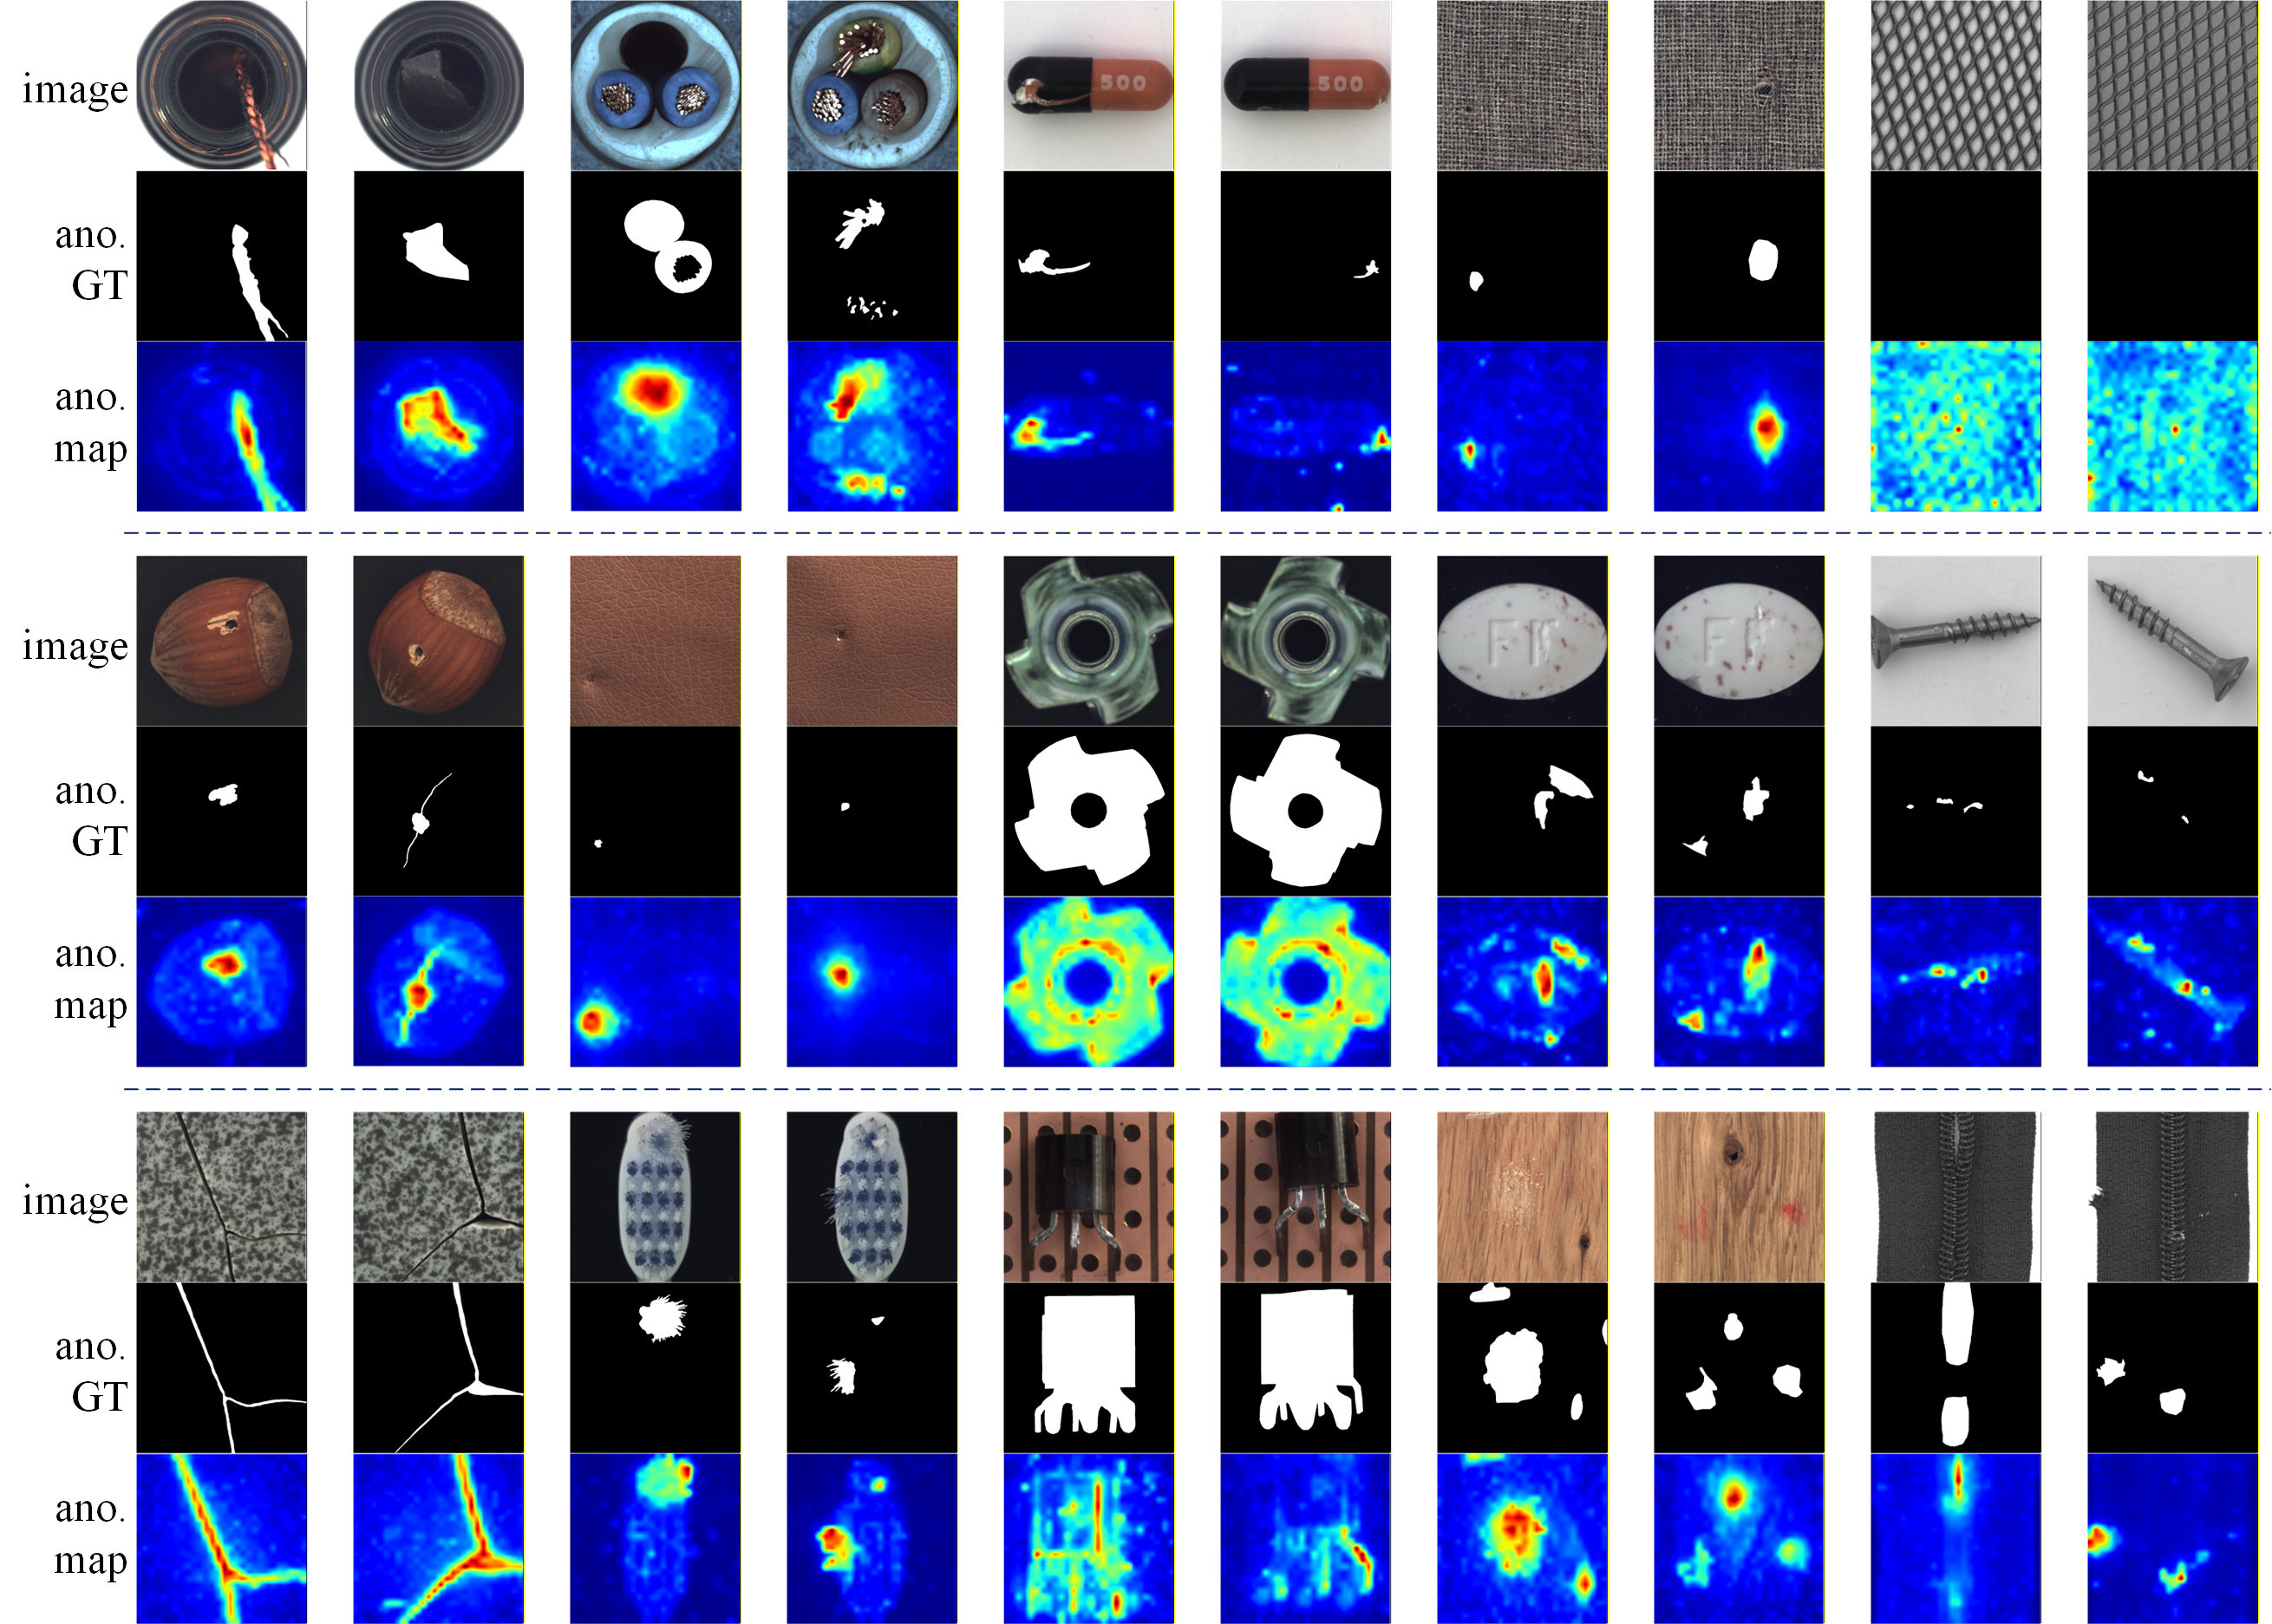
\includegraphics[width=1\linewidth]{figure/Figure_A1.png}
    \caption{Anomaly maps visualization on MVTec-AD. All samples are randomly chosen.}
    \label{fig:Figure_A1}
\end{figure}
\clearpage



\begin{figure}[p]
    \centering
    \includegraphics[width=1\linewidth]{figure/Figure_A2.png}
    \caption{Anomaly maps visualization on VisA. All samples are randomly chosen.}
    \label{fig:Figure_A2}
\end{figure}
\clearpage


\begin{figure}[p]
    \centering
    \includegraphics[width=1\linewidth]{figure/Figure_A3.png}
    \caption{Anomaly maps visualization on Real-IAD. All samples are randomly chosen.}
    \label{fig:Figure_A3}
\end{figure}
\clearpage

% You can have as much text here as you want. The main body must be at most $8$
% pages long. For the final version, one more page can be added. If you want, you
% can use an appendix like this one.

% The $\mathtt{\backslash onecolumn}$ command above can be kept in place if you
% prefer a one-column appendix, or can be removed if you prefer a two-column
% appendix.  Apart from this possible change, the style (font size, spacing,
% margins, page numbering, etc.) should be kept the same as the main body.
%%%%%%%%%%%%%%%%%%%%%%%%%%%%%%%%%%%%%%%%%%%%%%%%%%%%%%%%%%%%%%%%%%%%%%%%%%%%%%%
%%%%%%%%%%%%%%%%%%%%%%%%%%%%%%%%%%%%%%%%%%%%%%%%%%%%%%%%%%%%%%%%%%%%%%%%%%%%%%%


\end{document}

% This document was modified from the file originally made available by
% Pat Langley and Andrea Danyluk for ICML-2K. This version was created
% by Iain Murray in 2018, and modified by Alexandre Bouchard in
% 2019 and 2021 and by Csaba Szepesvari, Gang Niu and Sivan Sabato in 2022.
% Modified again in 2023 and 2024 by Sivan Sabato and Jonathan Scarlett.
% Previous contributors include Dan Roy, Lise Getoor and Tobias
% Scheffer, which was slightly modified from the 2010 version by
% Thorsten Joachims & Johannes Fuernkranz, slightly modified from the
% 2009 version by Kiri Wagstaff and Sam Roweis's 2008 version, which is
% slightly modified from Prasad Tadepalli's 2007 version which is a
% lightly changed version of the previous year's version by Andrew
% Moore, which was in turn edited from those of Kristian Kersting and
% Codrina Lauth. Alex Smola contributed to the algorithmic style files.
